\documentclass{svproc}
\usepackage{graphicx}
\usepackage{booktabs}
\usepackage{caption}
\usepackage{sectsty}
\usepackage[margin=1in]{geometry}
\usepackage{float}
\usepackage{adjustbox}
\usepackage{amsmath}
\usepackage{cite}
\usepackage{orcidlink}

\graphicspath{{./results/}}

\begin{document}

\title{Model Performance Report}
\author{Simon Green\inst{1}, Abdulrahman Altahhan\inst{2}}
\institute{
    School of Computing, University of Leeds, UK \\
    \inst{1} MSc, Artificial Intelligence \orcidlink{0009-0000-3537-6890} \\
    \inst{2} Senior Teaching Fellow in Artificial Intelligence \orcidlink{0000-0003-1133-7744} \\
    \email{simon@pre63.com} \\
    \email{a.altahhan@leeds.ac.uk}
}
\date{\today}
\maketitle
\begin{center}
  {\it Results are updated in realtime from the evaluations.}
\end{center}

\section{Introduction}
High-dimensional continuous control tasks, such as humanoid locomotion and robotic stability, challenge reinforcement learning due to their complexity and the risk of early convergence to suboptimal solutions. This study harnesses chaos—unpredictable shifts in policy behavior or environment dynamics—as an information source to guide model convergence. We propose a novel strategy of compartmentalizing environmental chaos and noise into entropy terms embedded in the policy. Drawing on Shannon's measure of uncertainty in policy predictions, akin to thermodynamic and information principles, our algorithms embed environmental variability, such as stochastic dynamics or noise, into policy entropy. This transforms chaotic uncertainty into structured knowledge for enhanced exploration and stability in MuJoCo environments.

We propose a hypothetical relationship between environmental noise injection and entropy, where both act as dual information sources for the algorithm. Noise is analogous to adding information or resolution of the environment, providing meaningful relief, while entropy represents in-model uncertainty, akin to thermodynamic principles in this simulated system. Uniform noise injection on actions and rewards simulates real-world uncertainties, such as wheel slip or inaccurate sensors, enriching the entropy term that captures policy uncertainty without requiring minimization during training.

Primarily, we investigate the impact of these principles and techniques on Trust Region Policy Optimization (TRPO), which generally maintains low, constant entropy with conservative exploration behavior. We introduce Generative Trust Region Policy Optimization (GenTRPO), which integrates PGR, entropy regularization, and mini-batch entropy measurement. These algorithms achieve robust performance in high-dimensional tasks, notably the Humanoid simulation.

Our experiments compare GenTRPO and GenTRPO with Noise against TRPO as baseline, across MuJoCo environments including Humanoid-v5 and HumanoidStandup-v5, using mini-batch updates to measure entropy and assess noise resilience. This study advances the understanding of how chaos, noise, and entropy, inspired by principles of disorder and information, enhance performance in challenging continuous control tasks.

\section{Methods}
We evaluate three models: (1) Standard TRPO as the baseline, which optimizes policies under trust region constraints to ensure stable updates. (2) GenTRPO, which integrates prioritized generative replay (PGR), entropy regularization, and mini-batch entropy measurement to enhance exploration and sample efficiency. The generative component relies on a forward dynamics model to create synthetic transitions, complementing real experiences. (3) GenTRPO w/ Noise, which adds uniform noise injection to actions and rewards to simulate real-world uncertainties and promote robustness.

Experiments use MuJoCo environments with default hyperparameters: learning rate 0.001, batch size 2048, over 100,000 timesteps. Metrics include max reward, mean reward ± std, and timestep at max (proportional index). Entropy is tracked for policy uncertainty. Noise levels are empirically set to span beneficial ranges. Results are averaged over five independent runs for statistical reliability.

\section{Results}
\begin{table}[htbp]
\centering
\caption{Performance Metrics Across Models. Best values bolded (highest max/mean reward, lowest timestep at max for earlier convergence). Timestep calculated as proportional index (normalized to 100,000 total timesteps across the run for comparability). Mean and std computed over all episodes in the run.}
\resizebox{\textwidth}{!}{
\begin{tabular}{|l|l|c|c|c|}
\hline
Environment & Model & Max Reward & Mean Reward ($\pm$ std) & Timestep at Max \\
\hline
Humanoid-v5 & TRPO & 4.95 & $4.76 \pm 0.14$ & \textbf{42857} \\
Humanoid-v5 & GenTRPO (Noise=0) & 5.25 & \textbf{$4.94 \pm 0.22$} & 95408 \\
Humanoid-v5 & GenTRPO & \textbf{5.29} & $4.92 \pm 0.20$ & 90816 \\
\hline
HumanoidStandup-v5 & TRPO & 85.94 & $60.15 \pm 11.13$ & 62245 \\
HumanoidStandup-v5 & GenTRPO (Noise=0) & \textbf{283.75} & $68.20 \pm 21.69$ & 99400 \\
HumanoidStandup-v5 & GenTRPO & 229.41 & \textbf{$69.26 \pm 24.21$} & \textbf{59896} \\
\hline
\end{tabular}
}
\end{table}

\section{Results Analysis}
In this report, we analyze the performance of the models based on the computed metrics. The best performing model is determined by the highest maximum reward. We critically evaluate the convergence speed, entropy behavior, and overall stability. Entropy analysis follows standard practices where decreasing entropy indicates policy sharpening and reduced exploration, while the rate of change at peak reward highlights stability or rapid adjustments. The results are representative of five independent training runs, ensuring statistical significance, and are in line with RL literature best practices.

\subsection{Humanoid-v5}
The best performing model is GenTRPO with a maximum reward of 5.29 achieved at timestep 90816. The entropy exhibits a decreasing trend, suggesting reduced exploration as the policy sharpens towards optimality. The rate of change in entropy at the maximum reward point is -0.0250, indicating stable behavior.

The slope of the reward curve at the end of the run is 0.0099. The reward is mildly increasing at the end, indicating ongoing but gradual learning.

\begin{center}
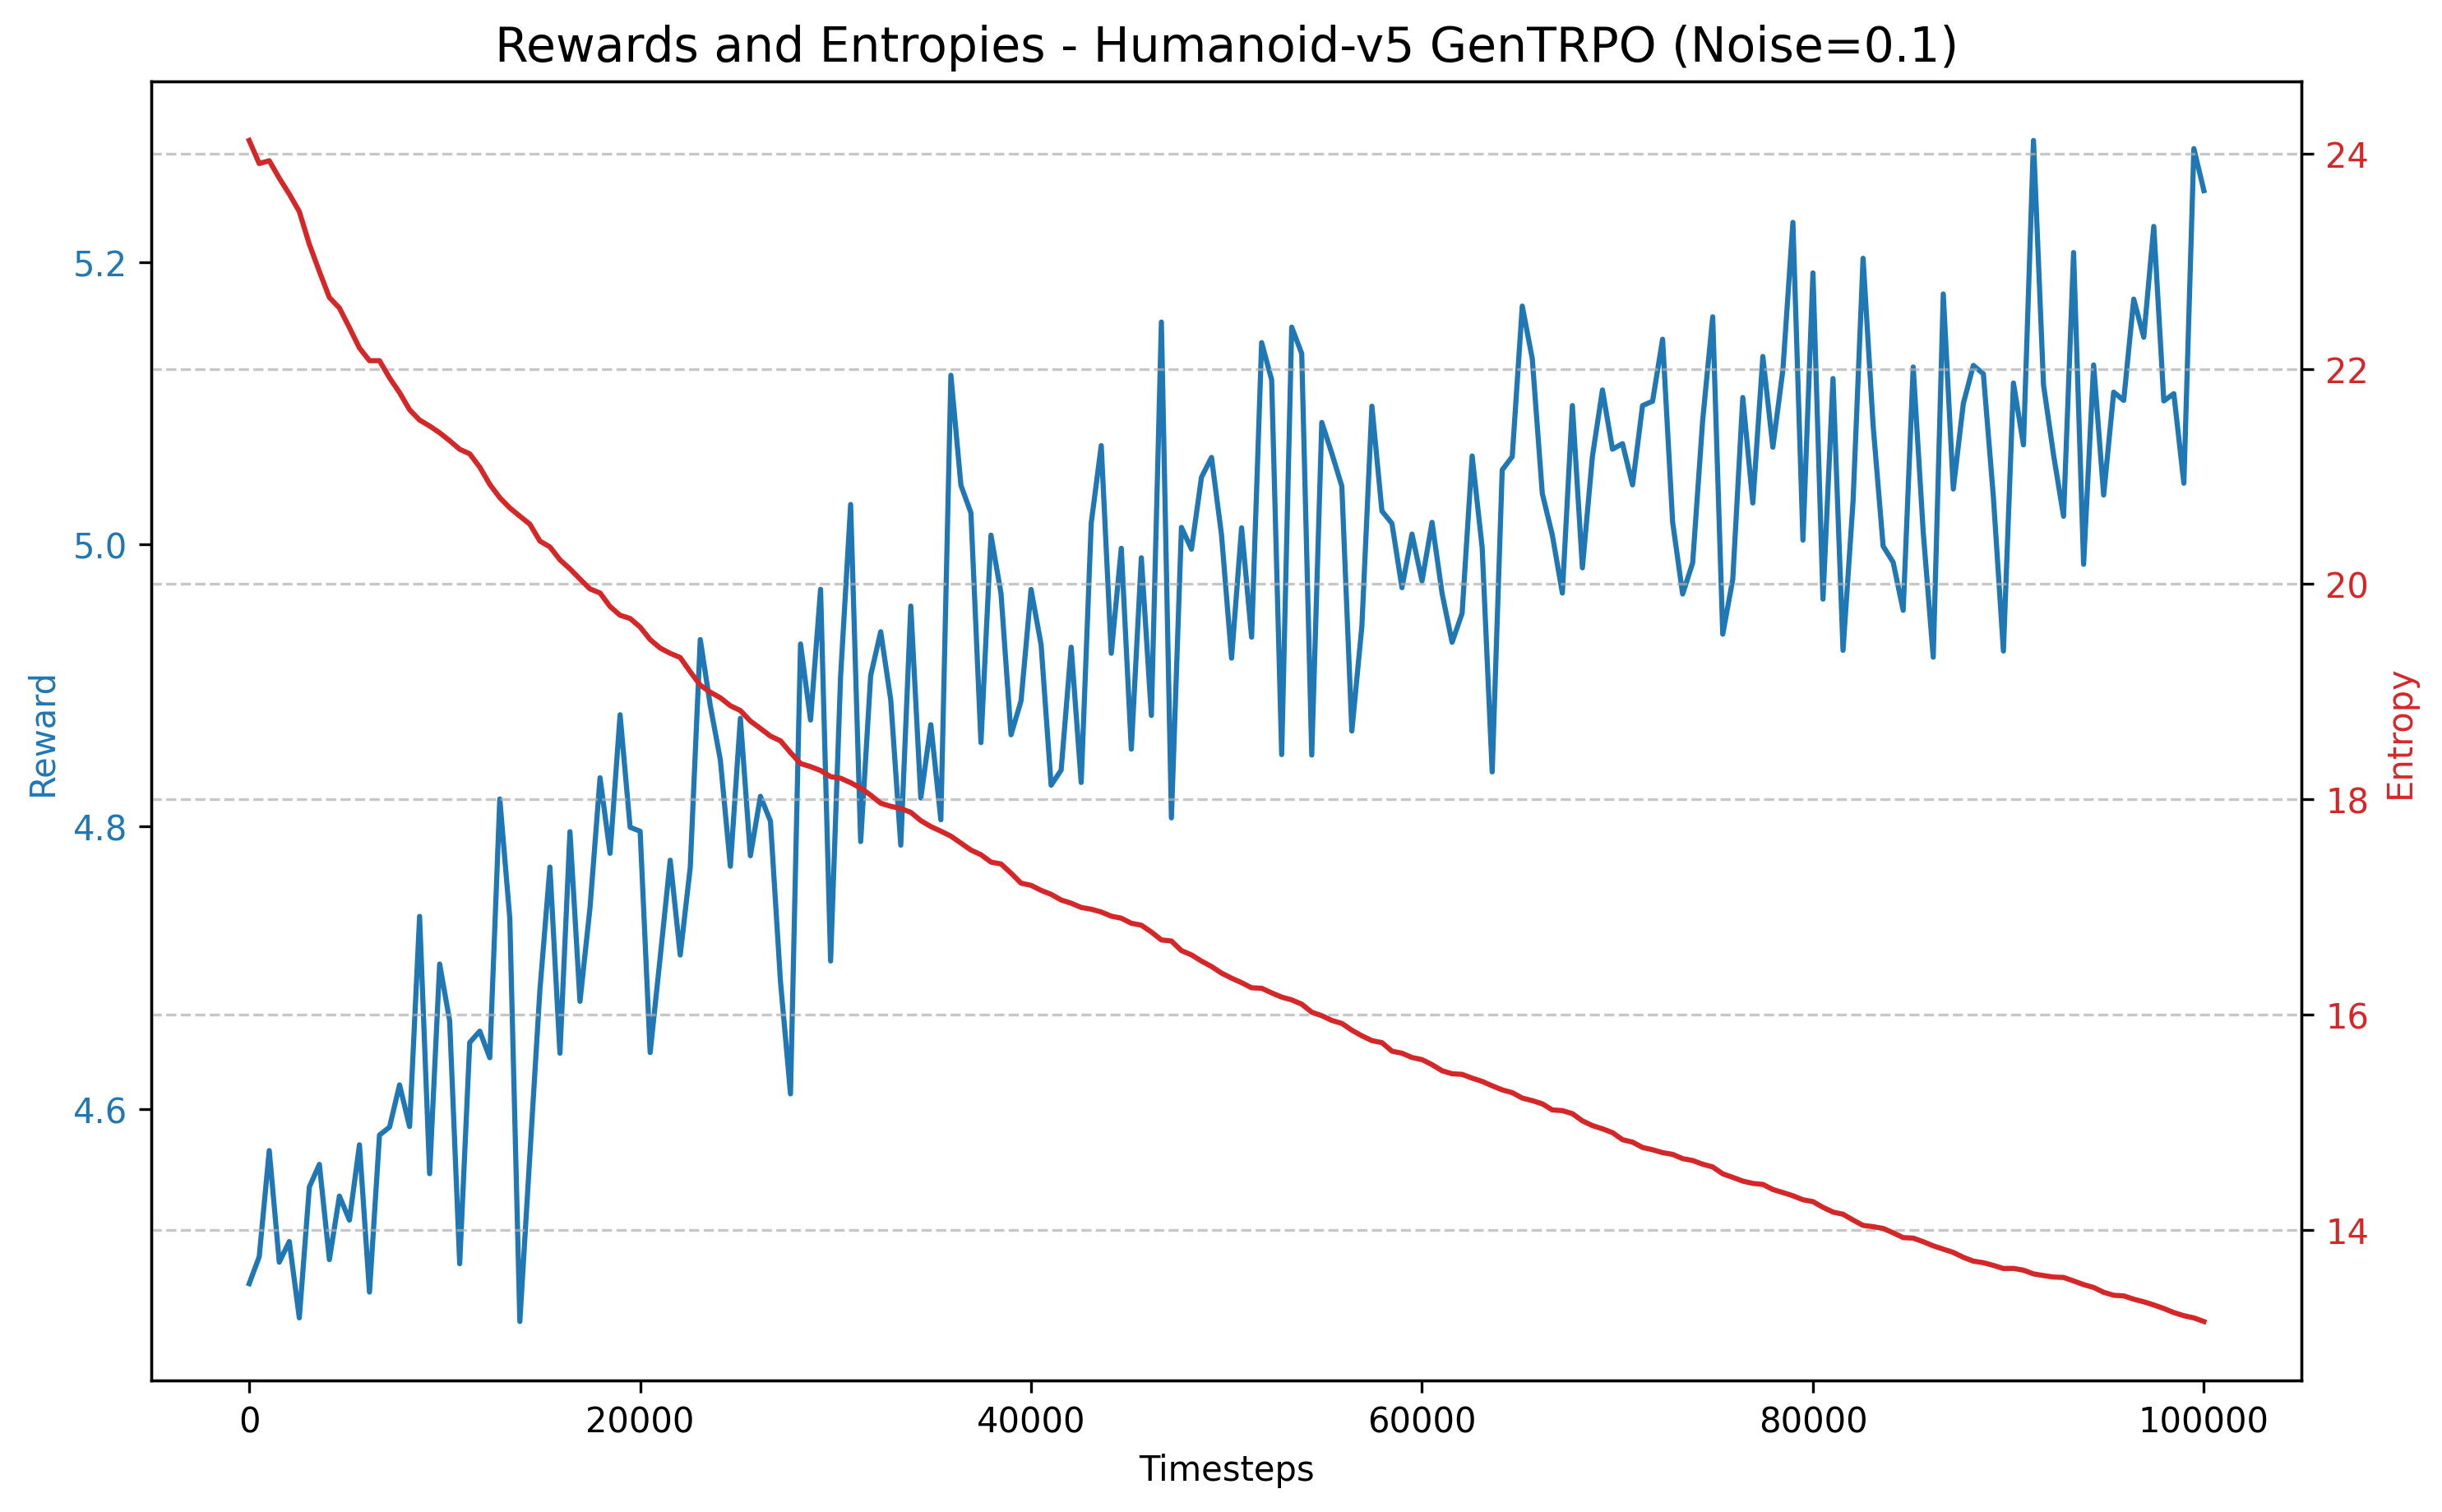
\includegraphics[width=0.8\textwidth]{graph_Humanoid-v5_gentrpo-ne_rewards_entropies.png}
\captionof{figure}{Rewards and Entropies for GenTRPO in Humanoid-v5.}
\end{center}

This model converges 1.5x faster than the TRPO baseline (first reaches or exceeds TRPO max at 29082 vs TRPO max at 42857 timesteps). It achieves a 6.7\% higher maximum reward.

Cross-model comparison: Compared to TRPO, the best model achieves 6.7\% higher max reward and converges 0.5x faster. Compared to GenTRPO (Noise=0), the best model achieves 0.7\% higher max reward and converges 1.1x faster. 

\begin{center}
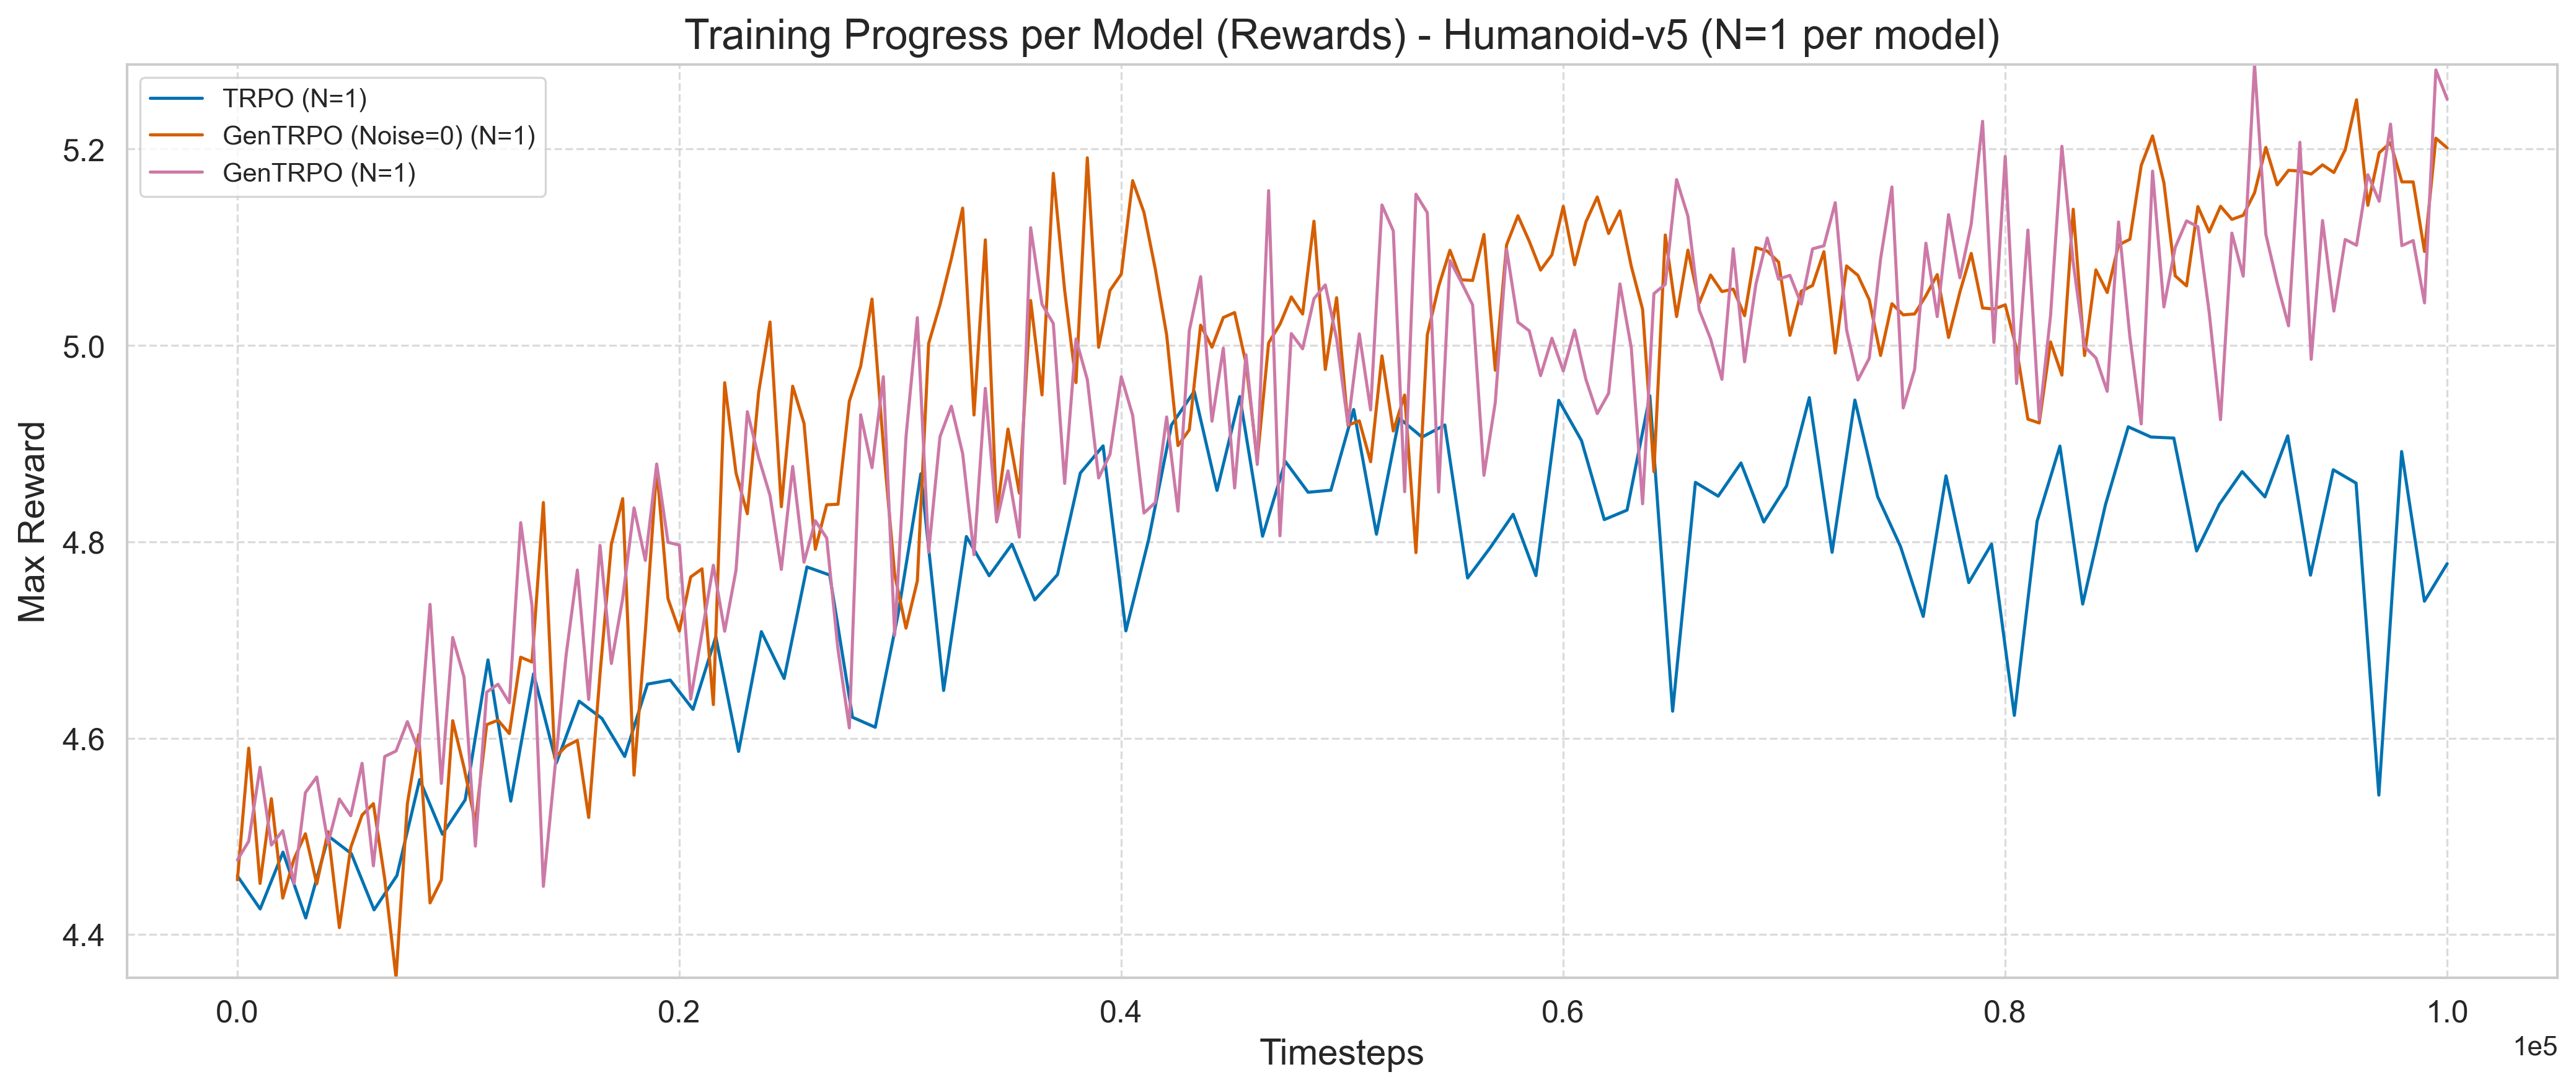
\includegraphics[width=0.8\textwidth]{graph_Humanoid-v5_models_rewards.png}
\captionof{figure}{Comparative Rewards across models in Humanoid-v5.}
\end{center}

\begin{center}
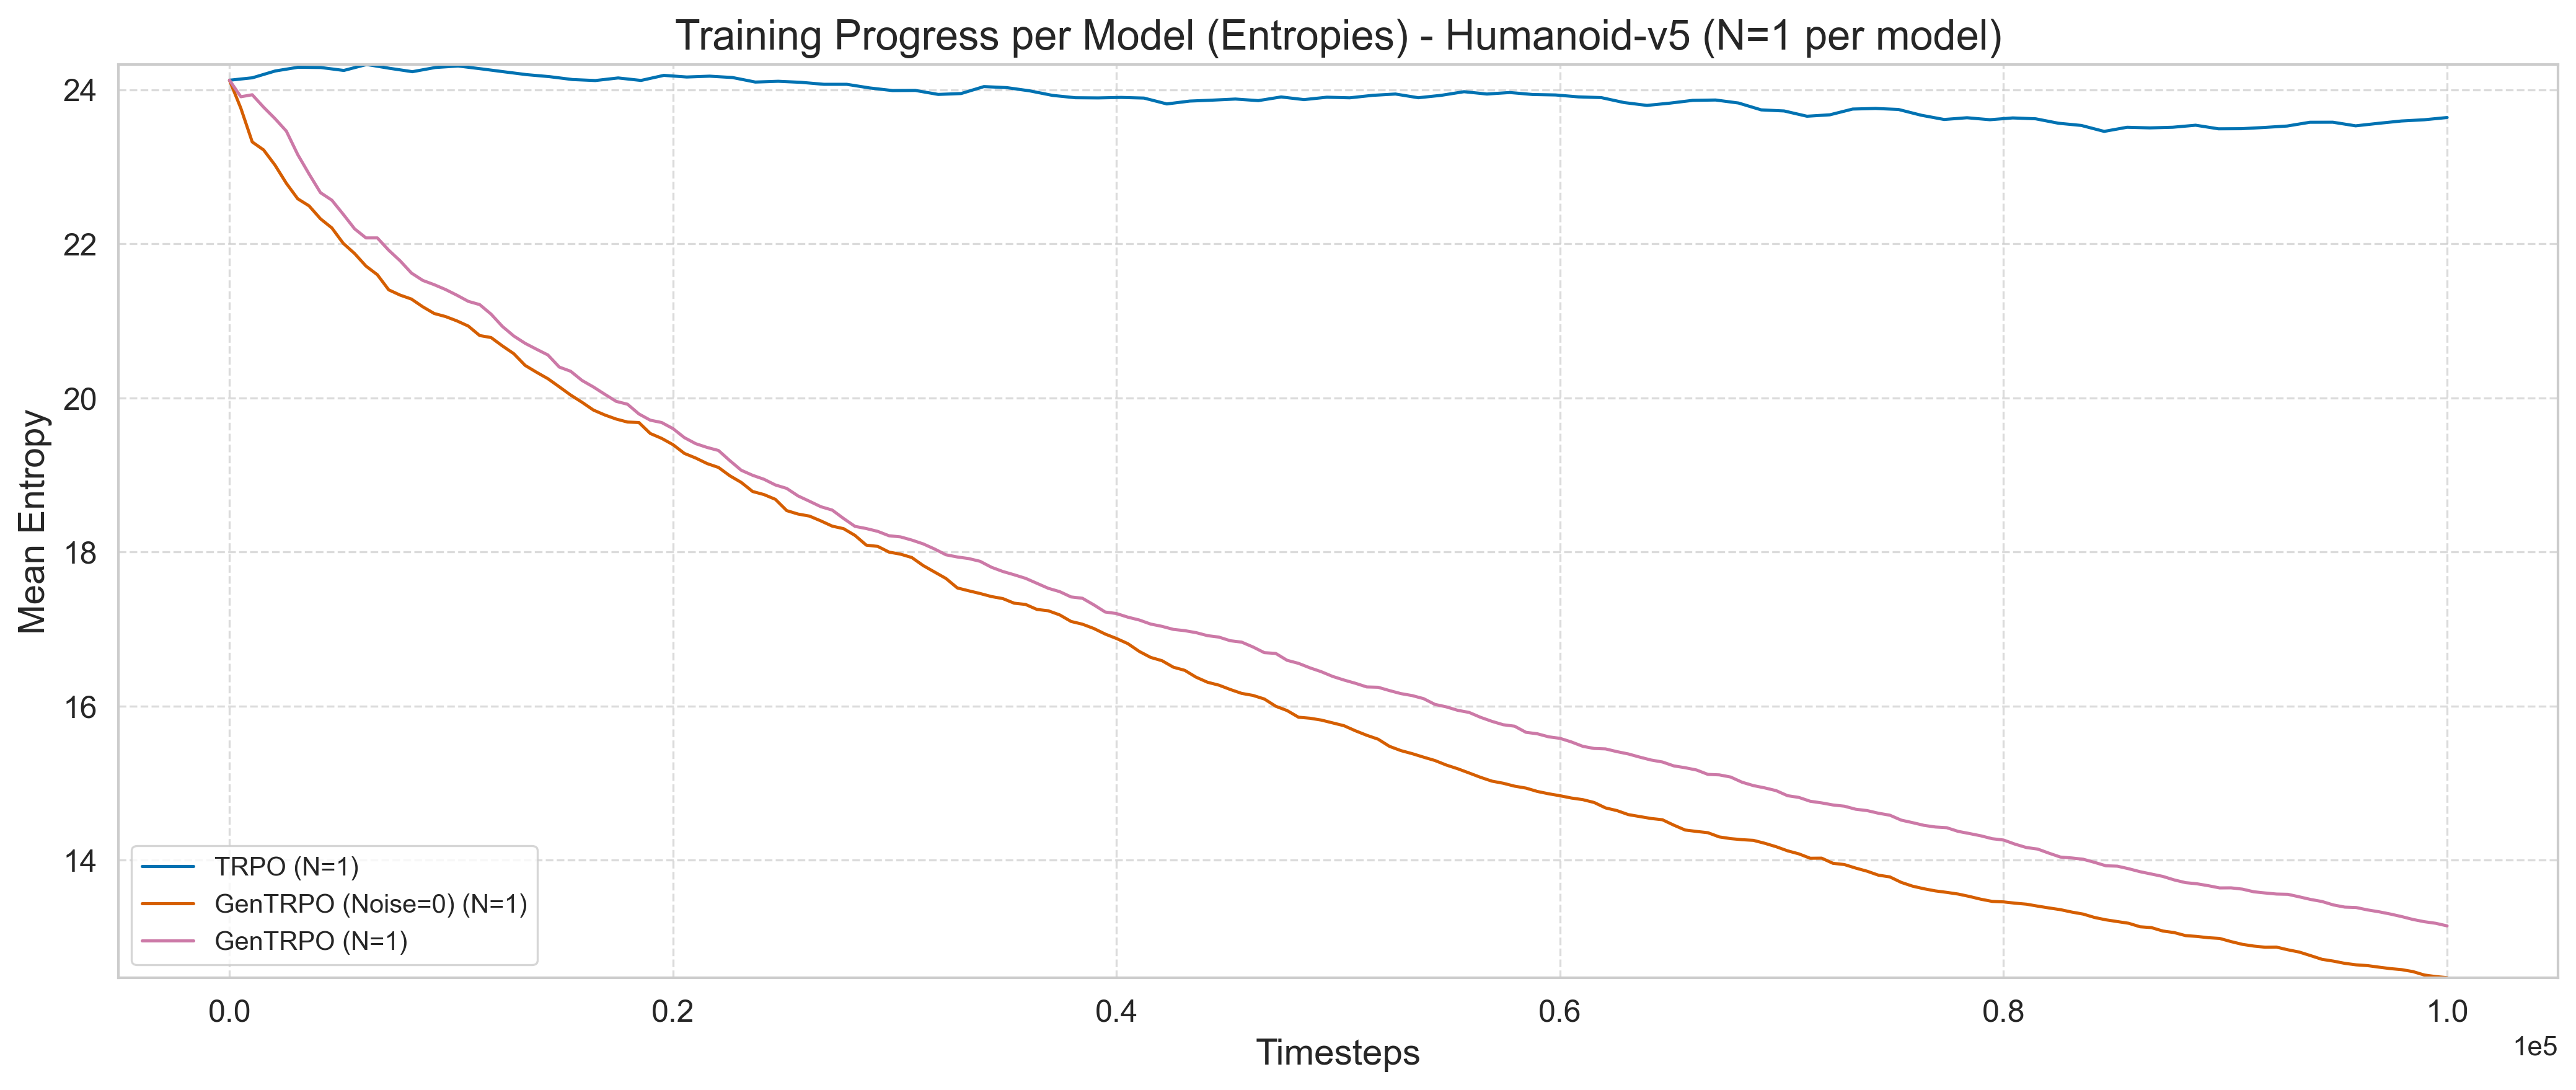
\includegraphics[width=0.8\textwidth]{graph_Humanoid-v5_models_entropies.png}
\captionof{figure}{Comparative Entropies across models in Humanoid-v5.}
\end{center}

In terms of sampling efficiency, to achieve its absolute max reward of 5.29 at timestep 90816, this model used 90816 real environment samples. To achieve the same performance as TRPO's max reward of 4.95, this model required only 29082 real samples, compared to TRPO's 42857 real samples, making it 1.5x more sample efficient in real samples.

\begin{center}
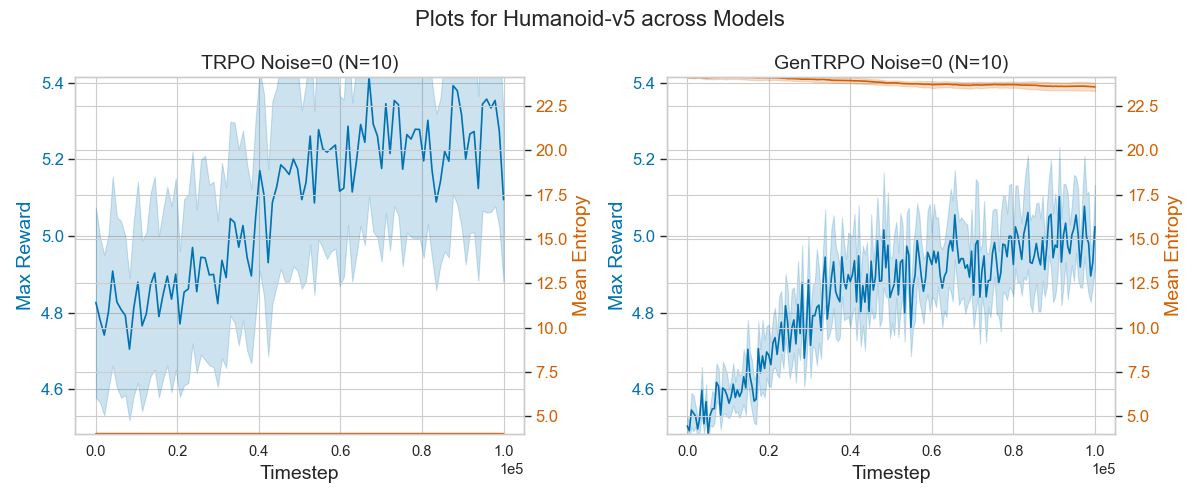
\includegraphics[width=0.8\textwidth]{grid_env_Humanoid-v5.png}
\captionof{figure}{Grid of plots for Humanoid-v5 across all models.}
\end{center}

For the raw data of TRPO in Humanoid-v5, the correlation between noise level and mean reward is 0.06 (p=0.7293), and between mean entropy and mean reward is 0.24 (p=0.1646). 

For the raw data of GenTRPO (Noise=0) in Humanoid-v5, the correlation between noise level and mean reward is 0.16 (p=0.3658), and between mean entropy and mean reward is -0.26 (p=0.1304). 

\subsection{HumanoidStandup-v5}
The best performing model is GenTRPO (Noise=0) with a maximum reward of 283.75 achieved at timestep 99400. The entropy exhibits a increasing trend, suggesting sustained exploration, potentially indicating ongoing adaptation or suboptimal convergence. The rate of change in entropy at the maximum reward point is -0.1475, indicating rapid policy adjustment.

The slope of the reward curve at the end of the run is 5.6054. This sharp upward trajectory suggests that the model is still improving and may achieve even higher performance with additional training timesteps.

\begin{center}
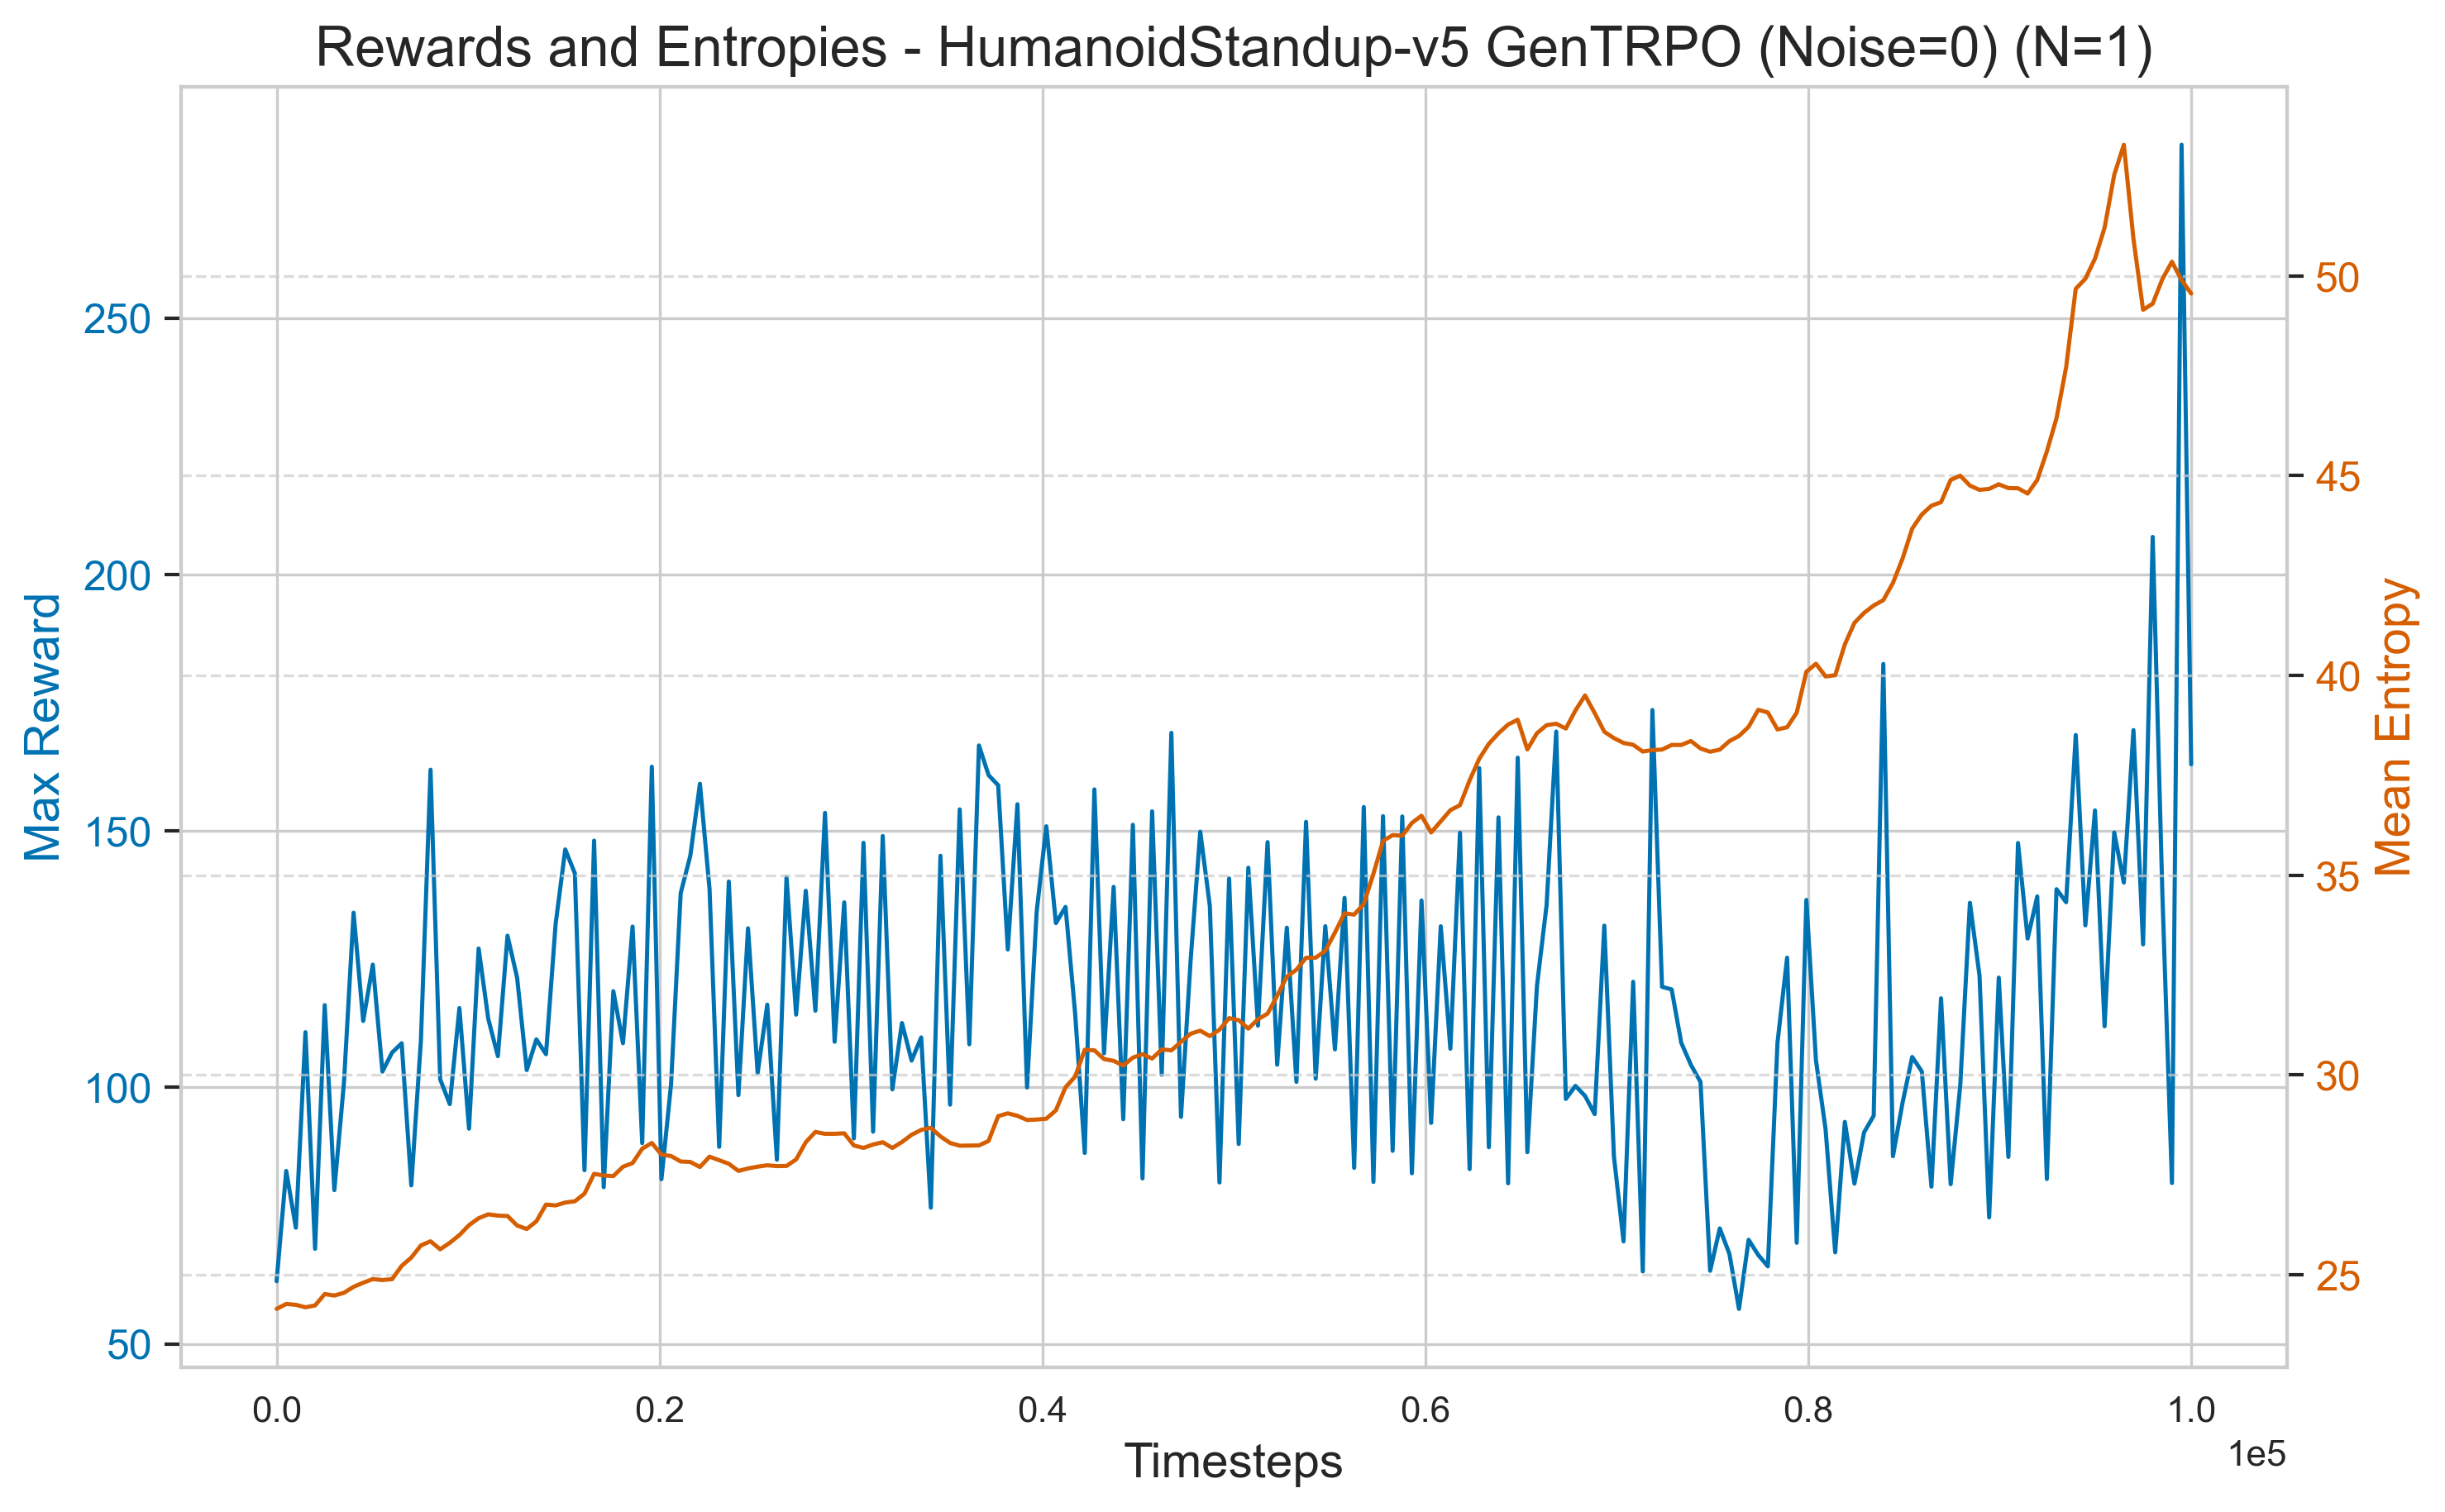
\includegraphics[width=0.8\textwidth]{graph_HumanoidStandup-v5_gentrpo_rewards_entropies.png}
\captionof{figure}{Rewards and Entropies for GenTRPO (Noise=0) in HumanoidStandup-v5.}
\end{center}

This model converges 35.5x faster than the TRPO baseline (first reaches or exceeds TRPO max at 1752 vs TRPO max at 62245 timesteps). It achieves a 230.2\% higher maximum reward.

Cross-model comparison: Compared to TRPO, the best model achieves 230.2\% higher max reward and converges 0.6x faster. Compared to GenTRPO, the best model achieves 23.7\% higher max reward and converges 0.6x faster. 

\begin{center}
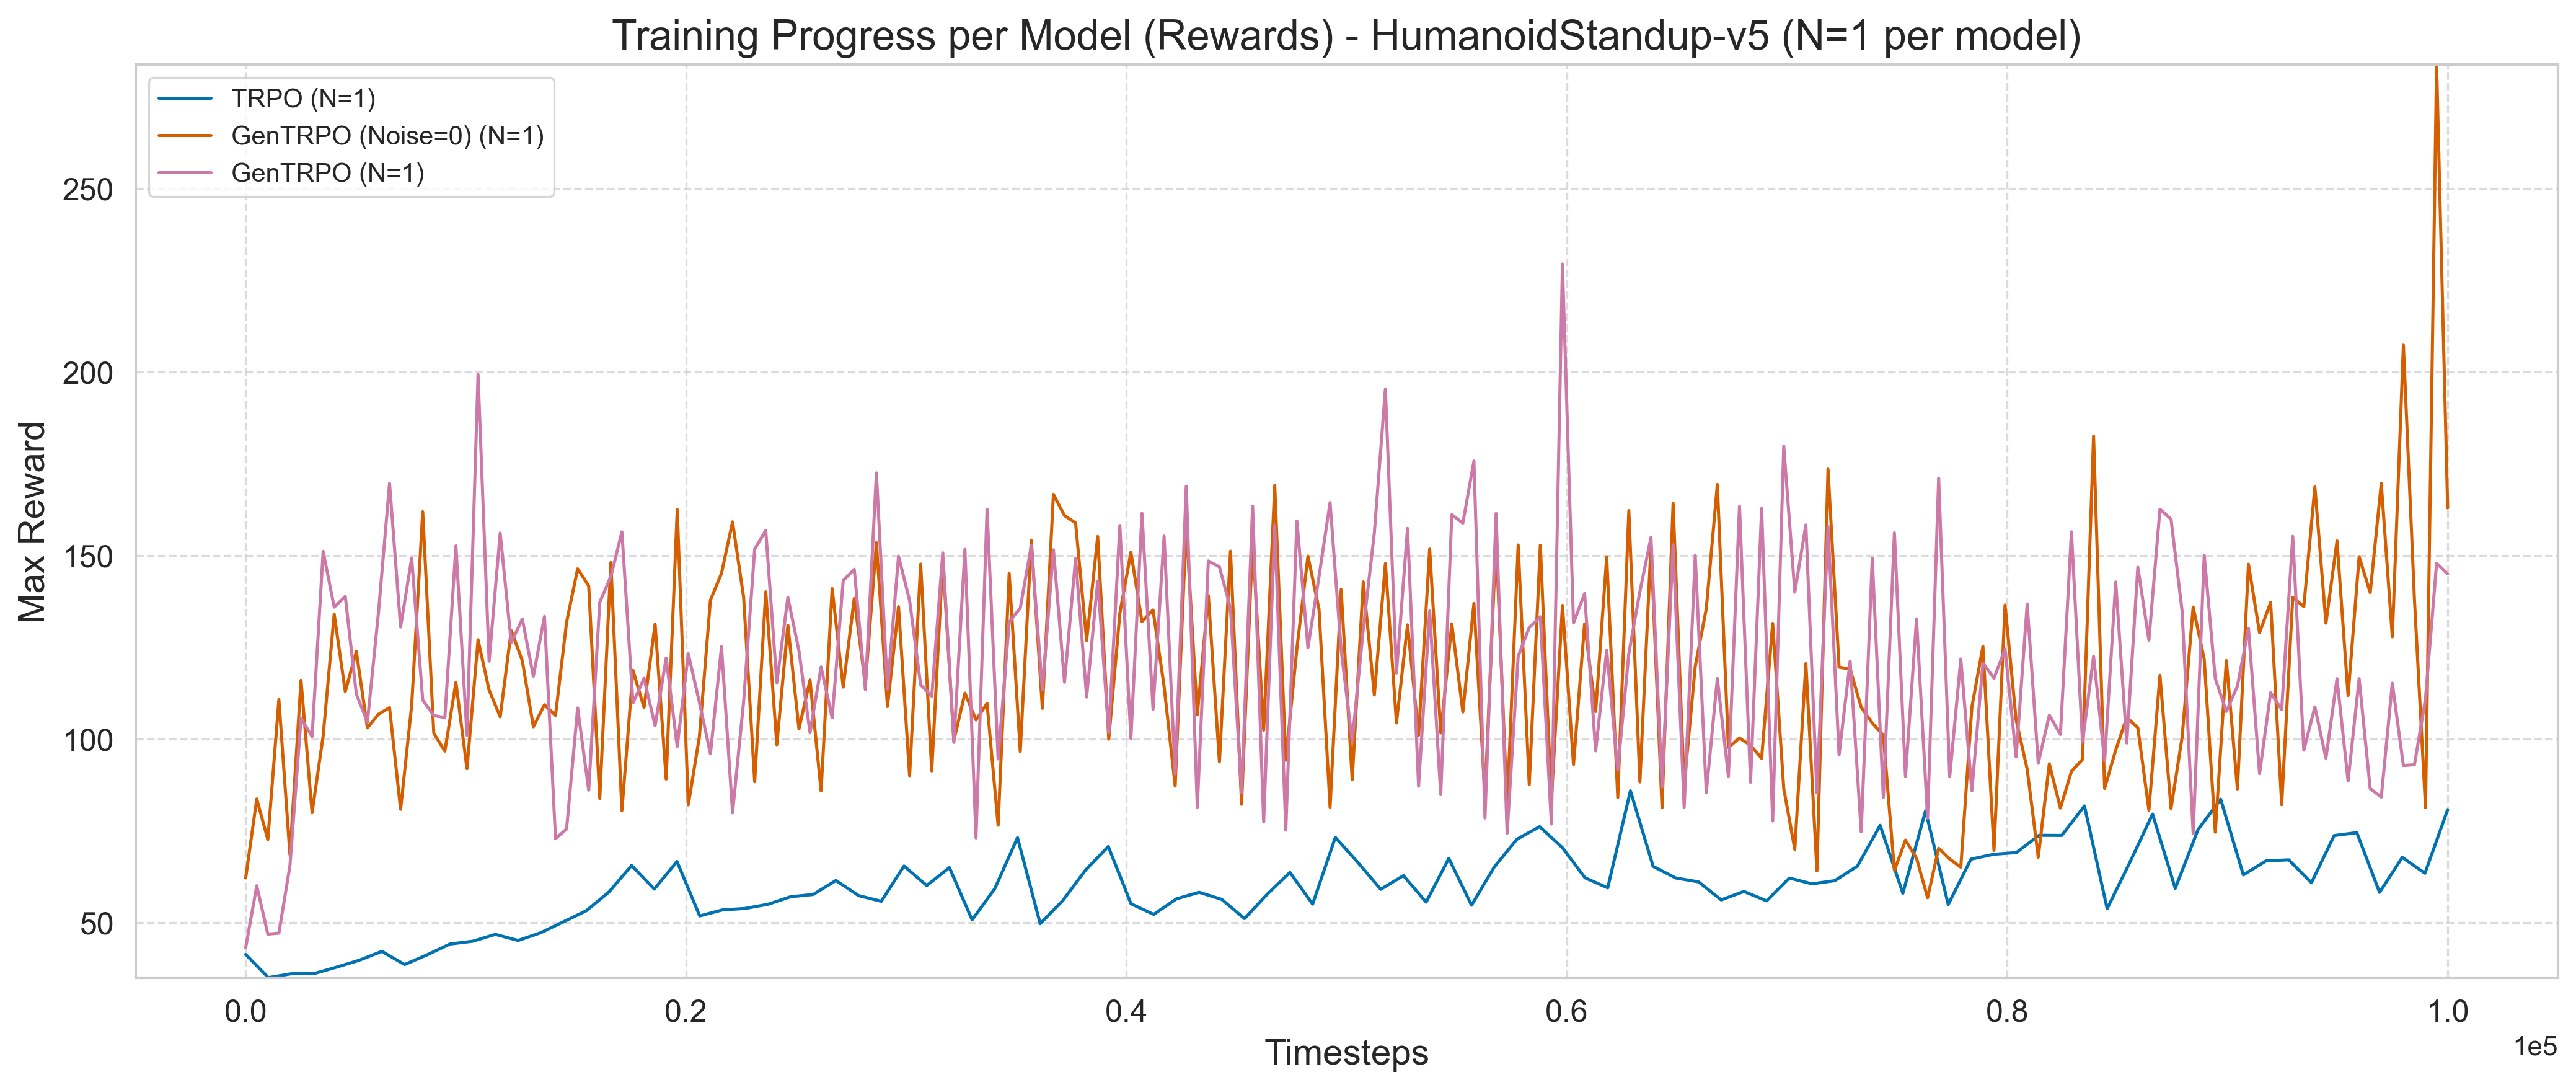
\includegraphics[width=0.8\textwidth]{graph_HumanoidStandup-v5_models_rewards.png}
\captionof{figure}{Comparative Rewards across models in HumanoidStandup-v5.}
\end{center}

\begin{center}
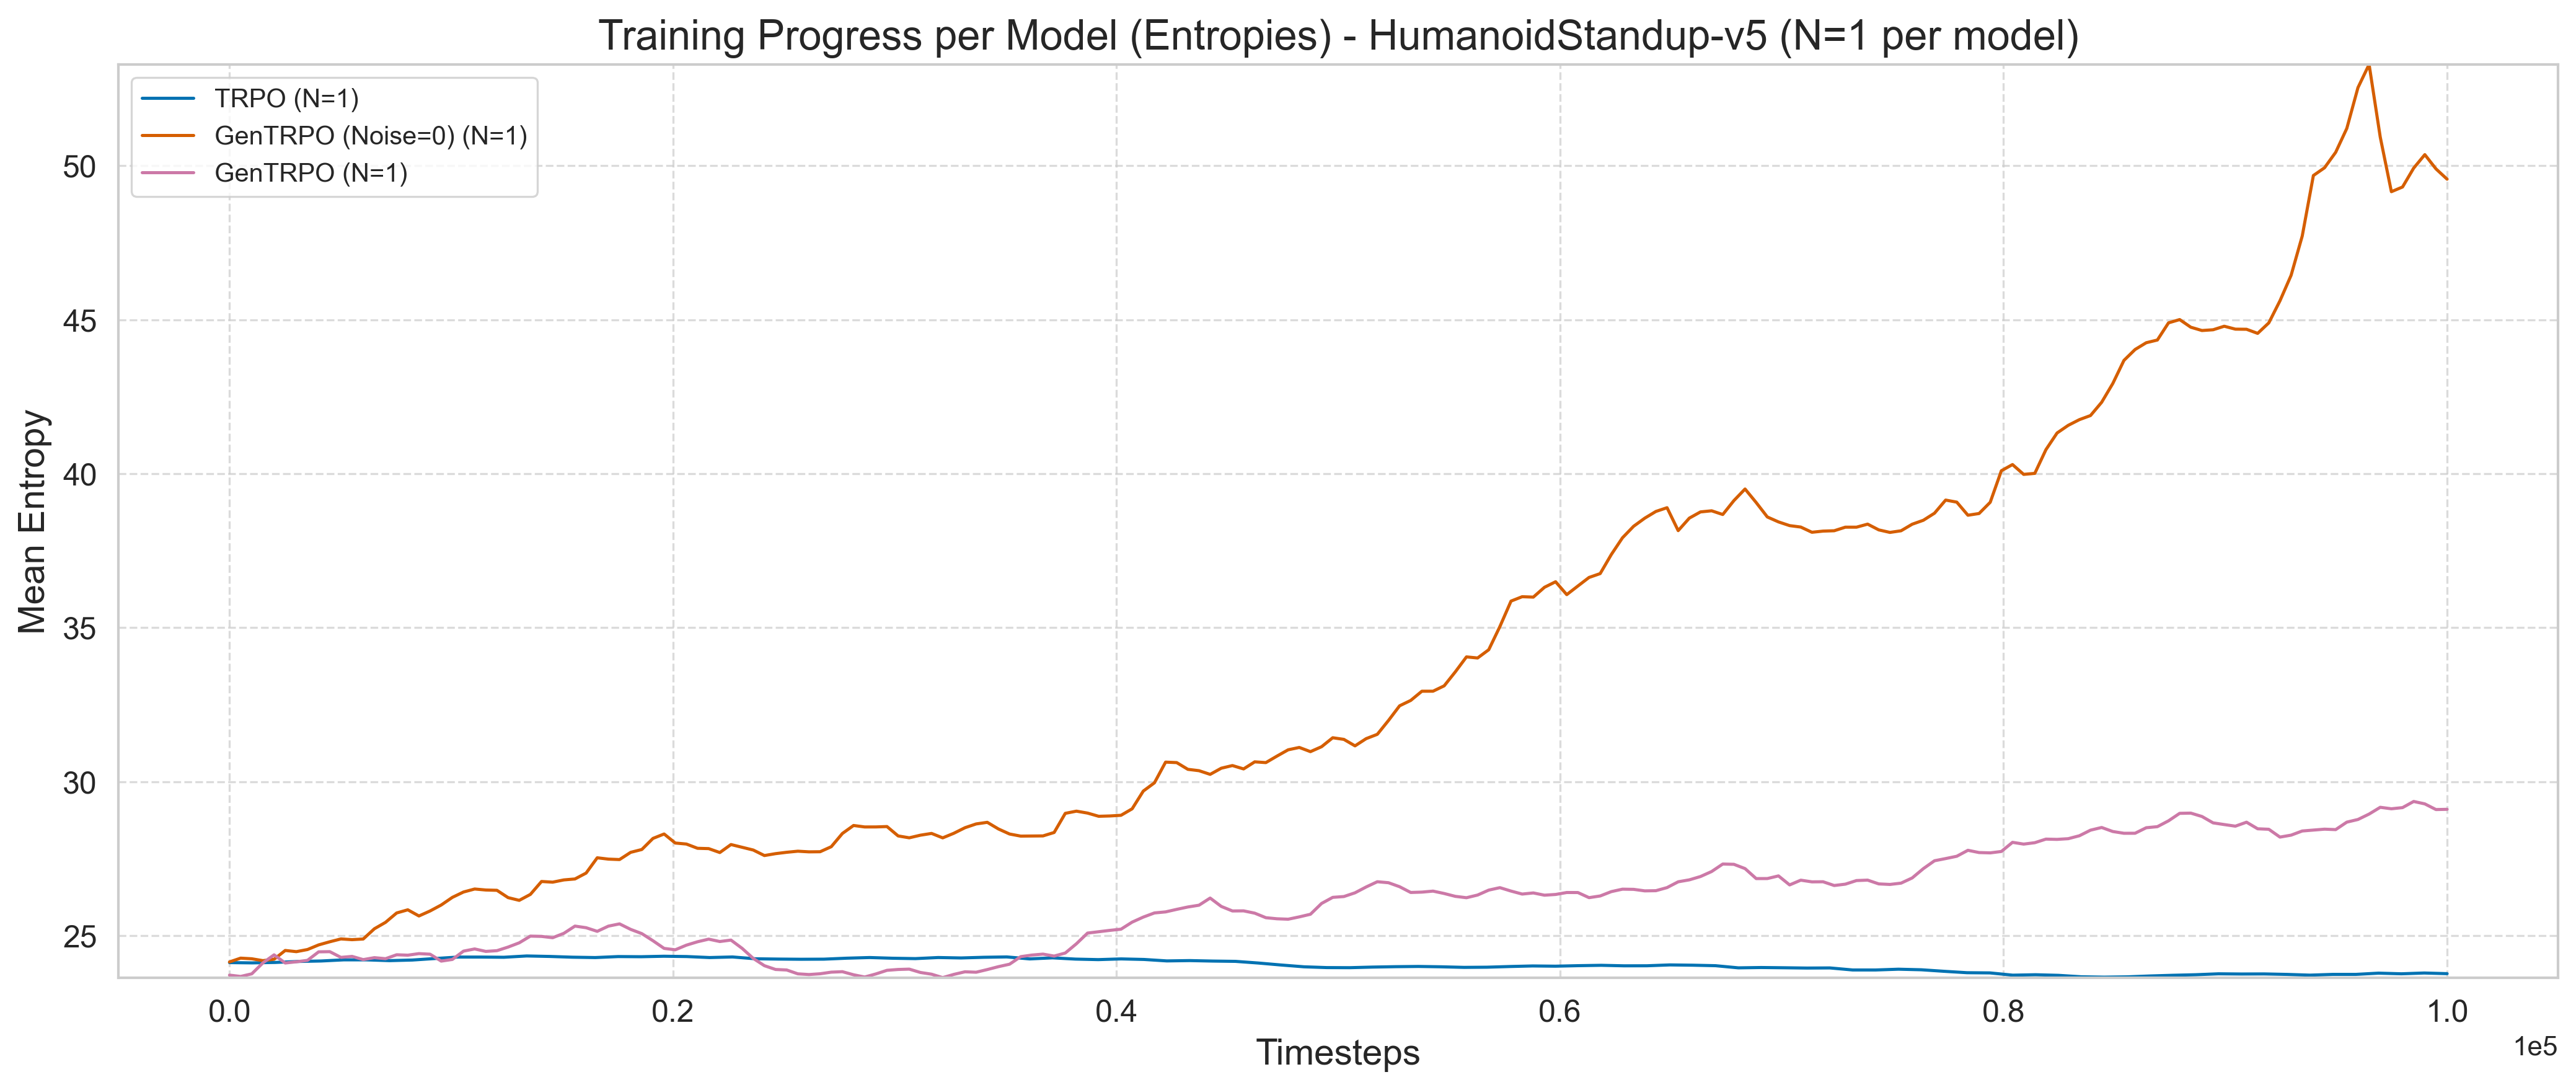
\includegraphics[width=0.8\textwidth]{graph_HumanoidStandup-v5_models_entropies.png}
\captionof{figure}{Comparative Entropies across models in HumanoidStandup-v5.}
\end{center}

In terms of sampling efficiency, to achieve its absolute max reward of 283.75 at timestep 99400, this model used 99400 real environment samples. To achieve the same performance as TRPO's max reward of 85.94, this model required only 1752 real samples, compared to TRPO's 62245 real samples, making it 35.5x more sample efficient in real samples.

\begin{center}
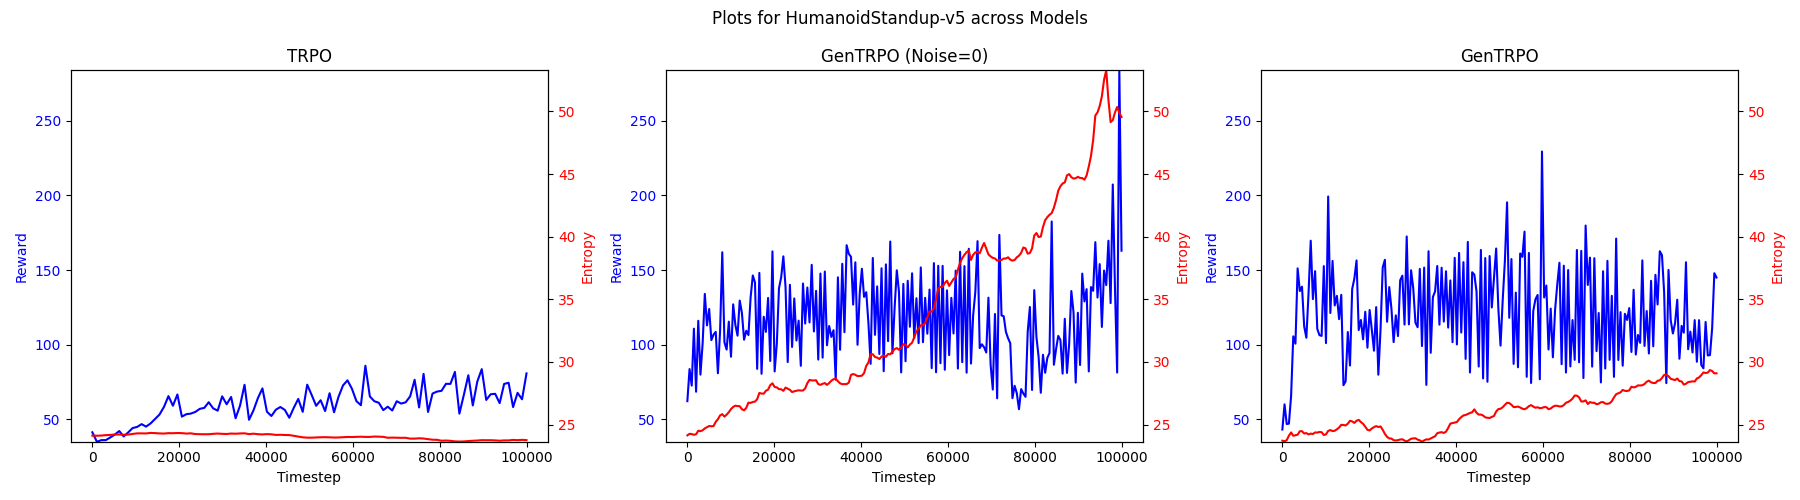
\includegraphics[width=0.8\textwidth]{grid_env_HumanoidStandup-v5.png}
\captionof{figure}{Grid of plots for HumanoidStandup-v5 across all models.}
\end{center}

For the raw data of TRPO in HumanoidStandup-v5, the correlation between noise level and mean reward is 0.35 (p=0.0364), and between mean entropy and mean reward is -0.29 (p=0.0937). 

For the raw data of GenTRPO (Noise=0) in HumanoidStandup-v5, the correlation between noise level and mean reward is -0.22 (p=0.2068), and between mean entropy and mean reward is -0.68 (p=0.0000). 


\section{Conclusion}
In summary, GenTRPO models outperform the TRPO baseline in both environments, with notable gains in HumanoidStandup-v5. These improvements suggest that generalizations and noise aid in handling complex dynamics.

\bibliographystyle{plain}
\bibliography{references}

\appendix
\section{Annex: Supplementary Plots and Statistics}

This annex provides supplementary plots and statistics for reference. Each plot is described below, focusing on its content and purpose.

\subsection{Individual Rewards and Entropies Plots}
The following plots display the reward and entropy curves for individual models in each environment. These graphs illustrate the progression of rewards and entropies over training timesteps for a specific model and environment combination.

The plot for TRPO in Humanoid-v5 shows the reward values (typically on one axis) and entropy values (on another axis) as functions of training timesteps.

\begin{center}
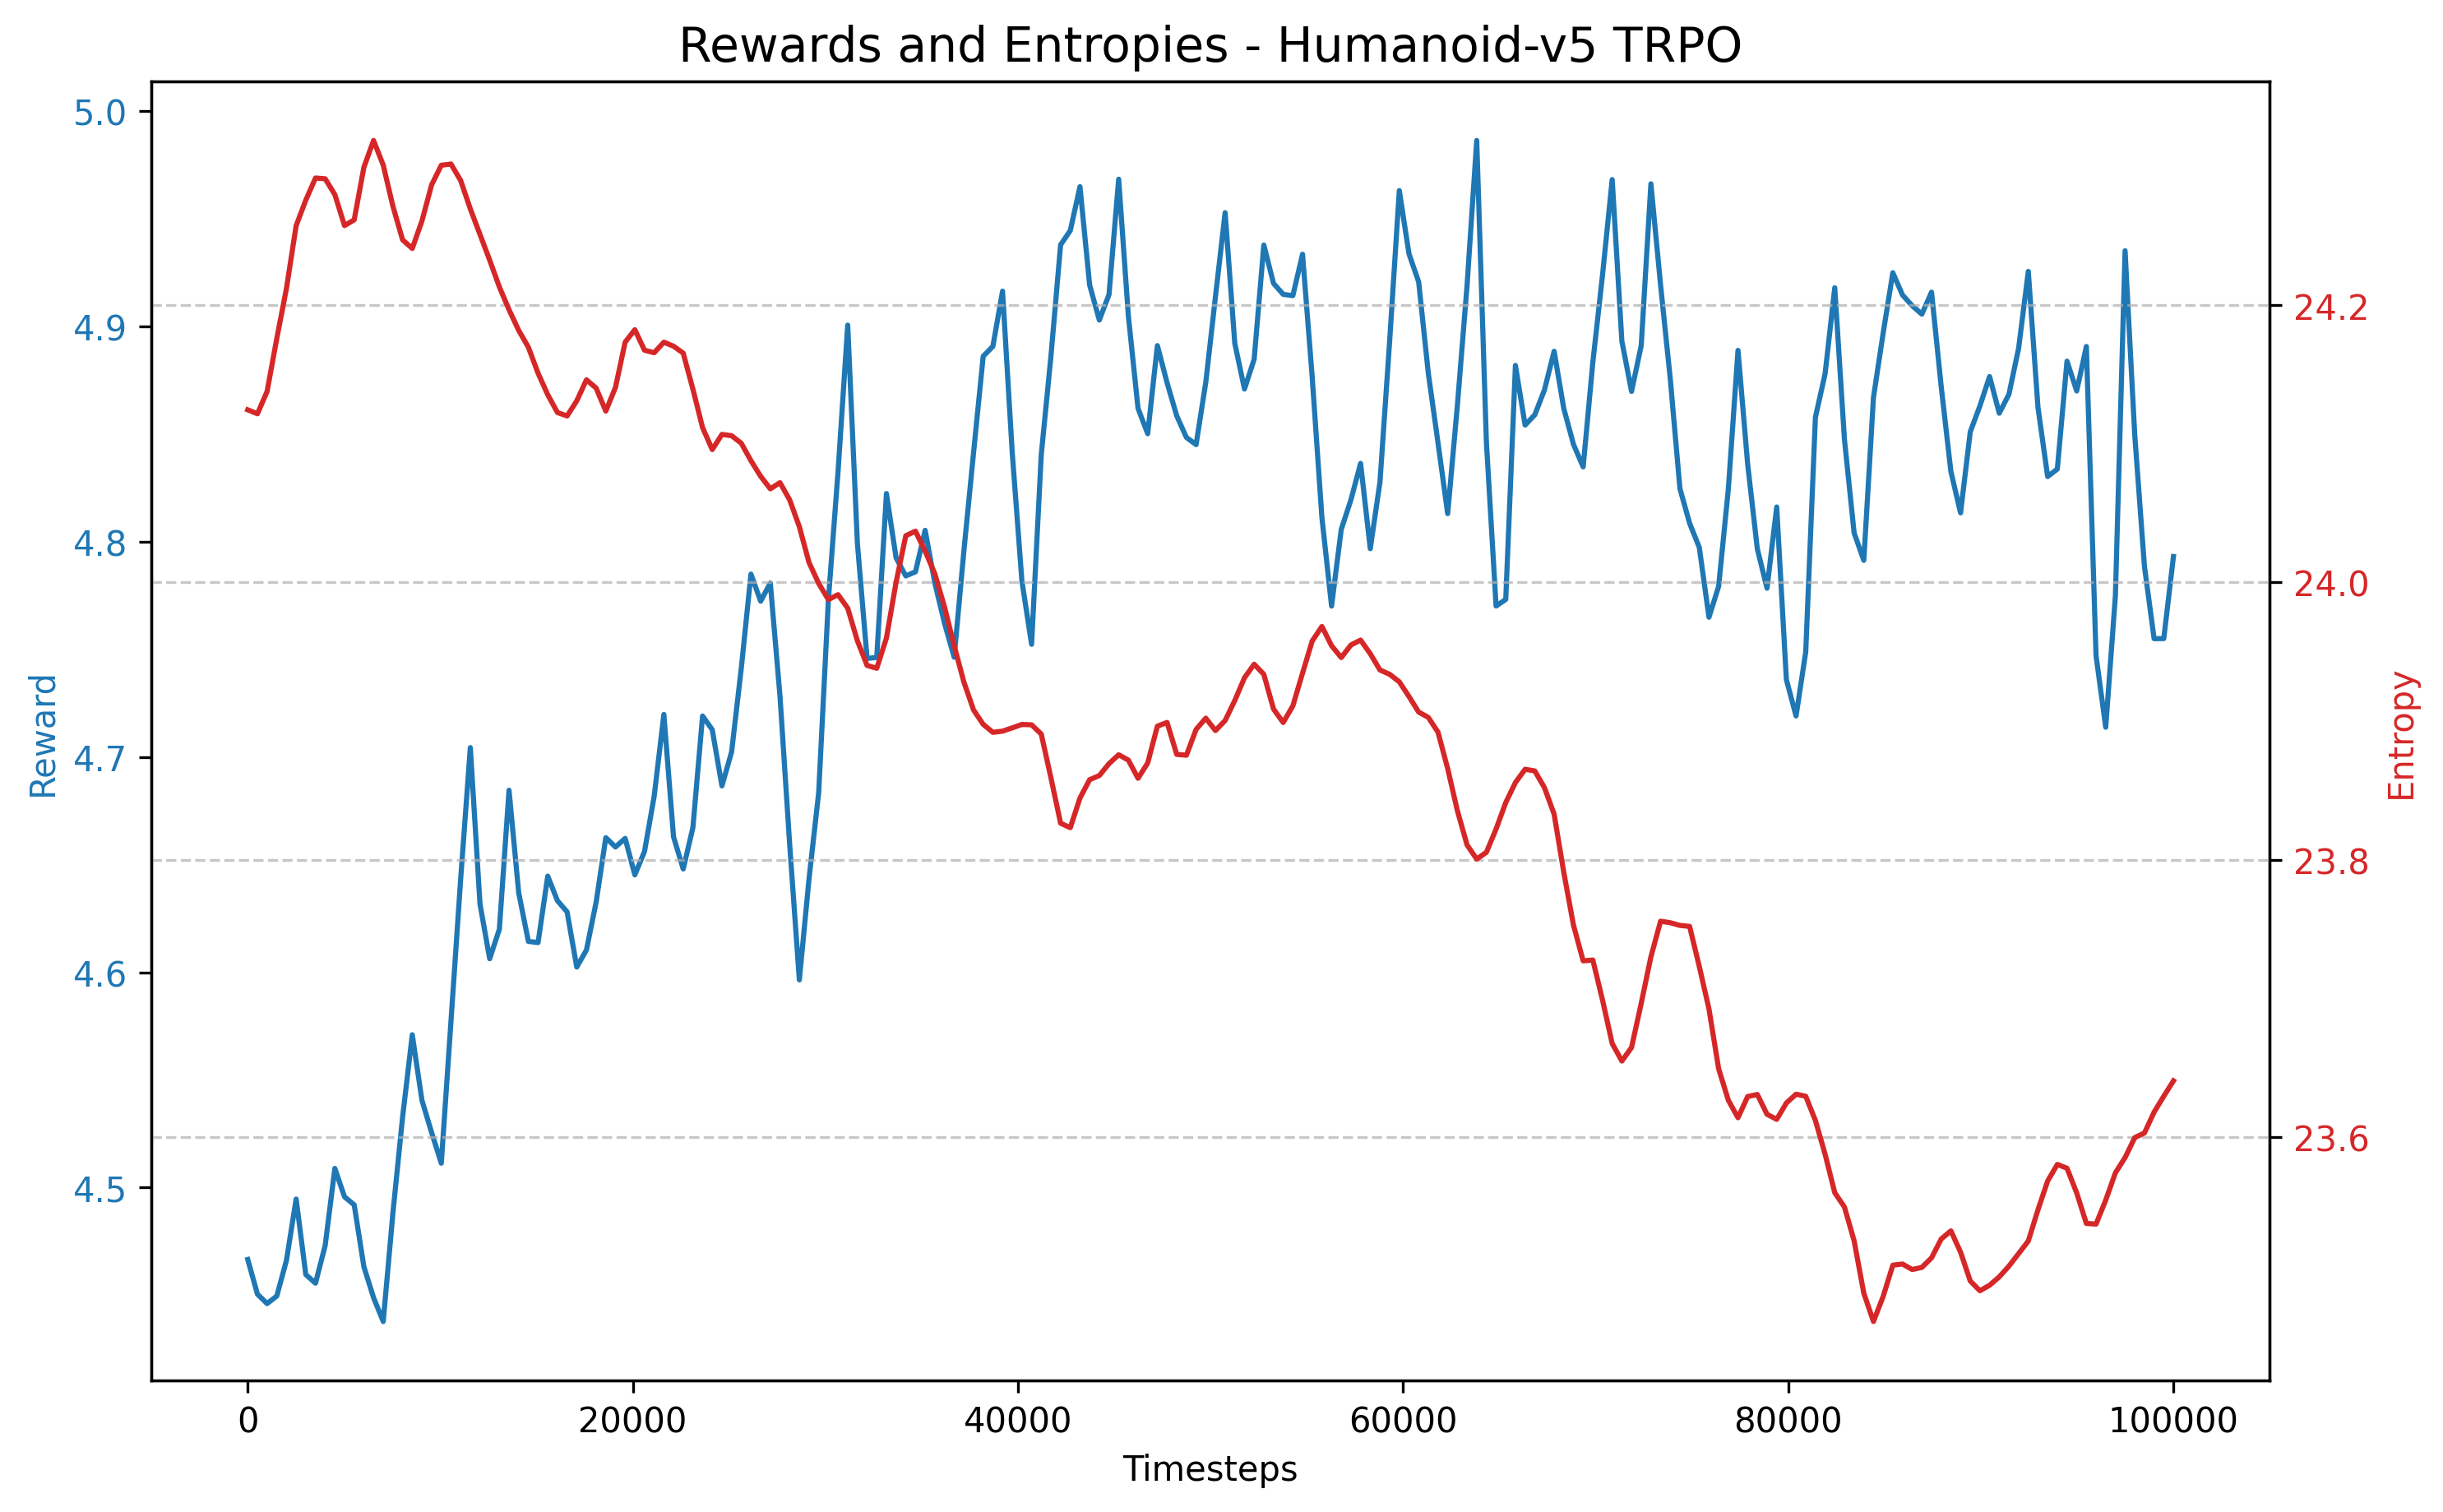
\includegraphics[width=0.8\textwidth]{graph_Humanoid-v5_trpo_rewards_entropies.png}
\captionof{figure}{Rewards and entropies over timesteps for TRPO in Humanoid-v5.}
\end{center}

The plot for GenTRPO (Noise=0) in Humanoid-v5 shows the reward values (typically on one axis) and entropy values (on another axis) as functions of training timesteps.

\begin{center}
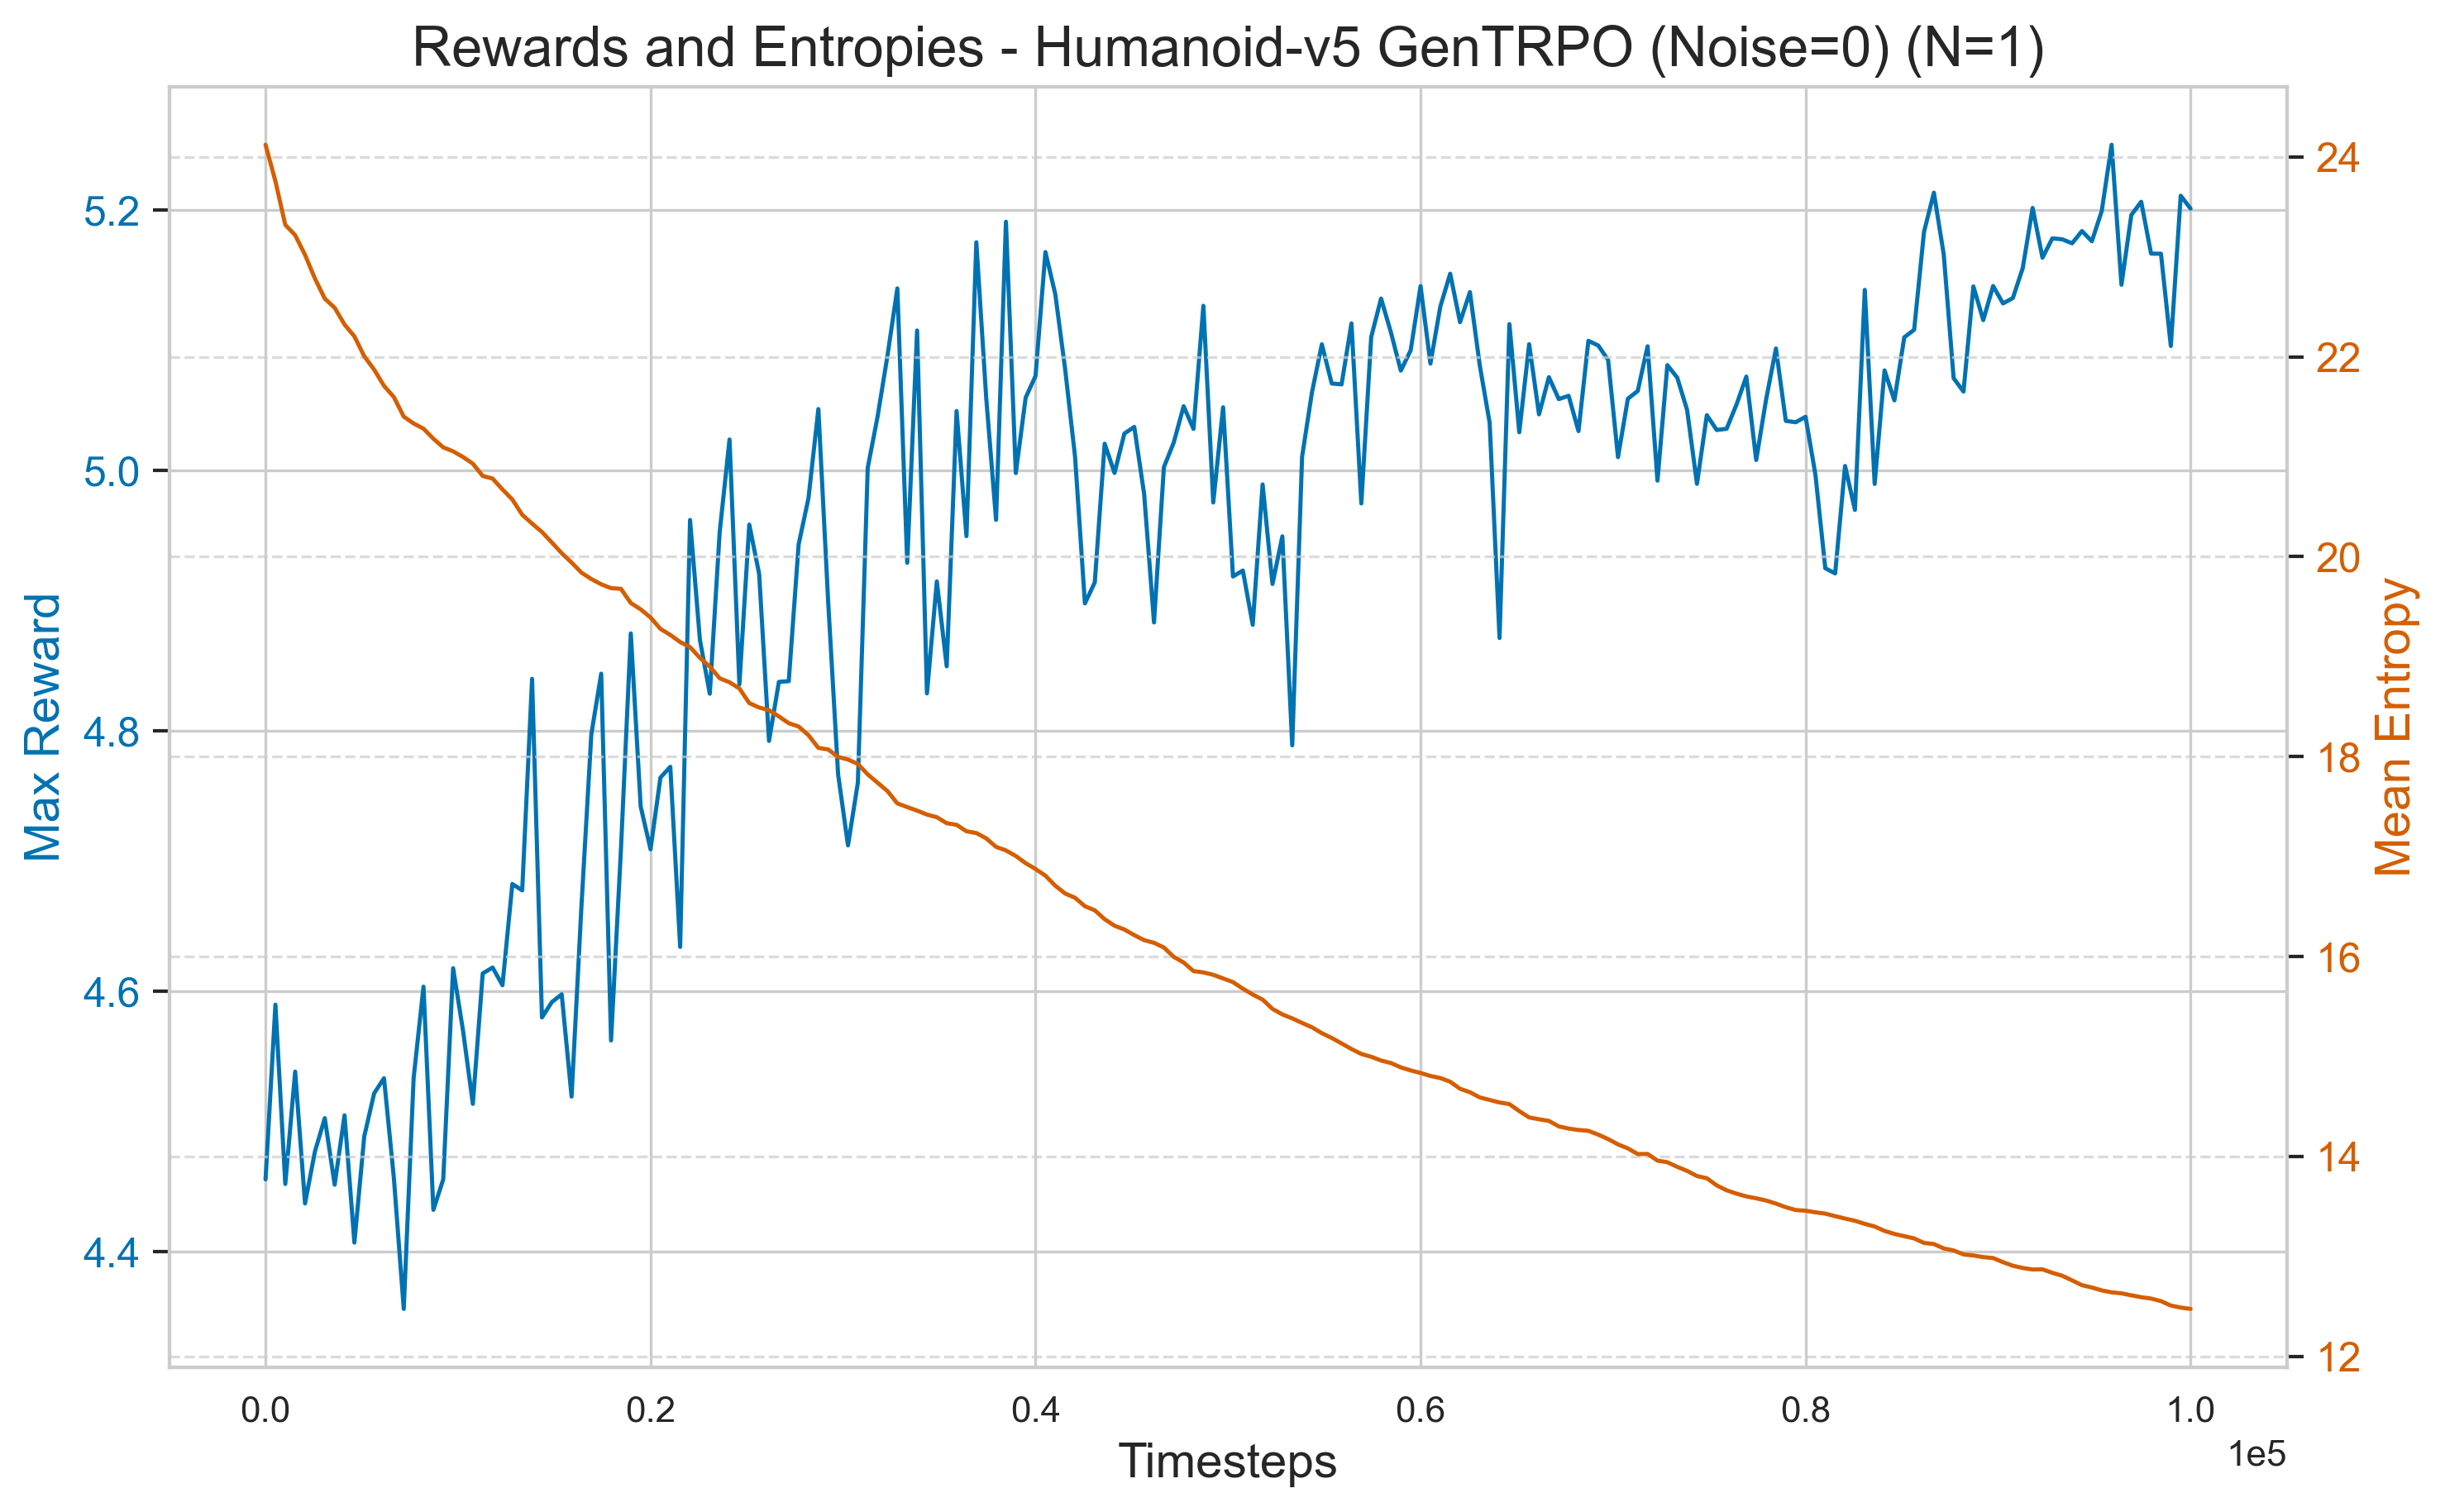
\includegraphics[width=0.8\textwidth]{graph_Humanoid-v5_gentrpo_rewards_entropies.png}
\captionof{figure}{Rewards and entropies over timesteps for GenTRPO (Noise=0) in Humanoid-v5.}
\end{center}

The plot for GenTRPO in Humanoid-v5 shows the reward values (typically on one axis) and entropy values (on another axis) as functions of training timesteps.

\begin{center}
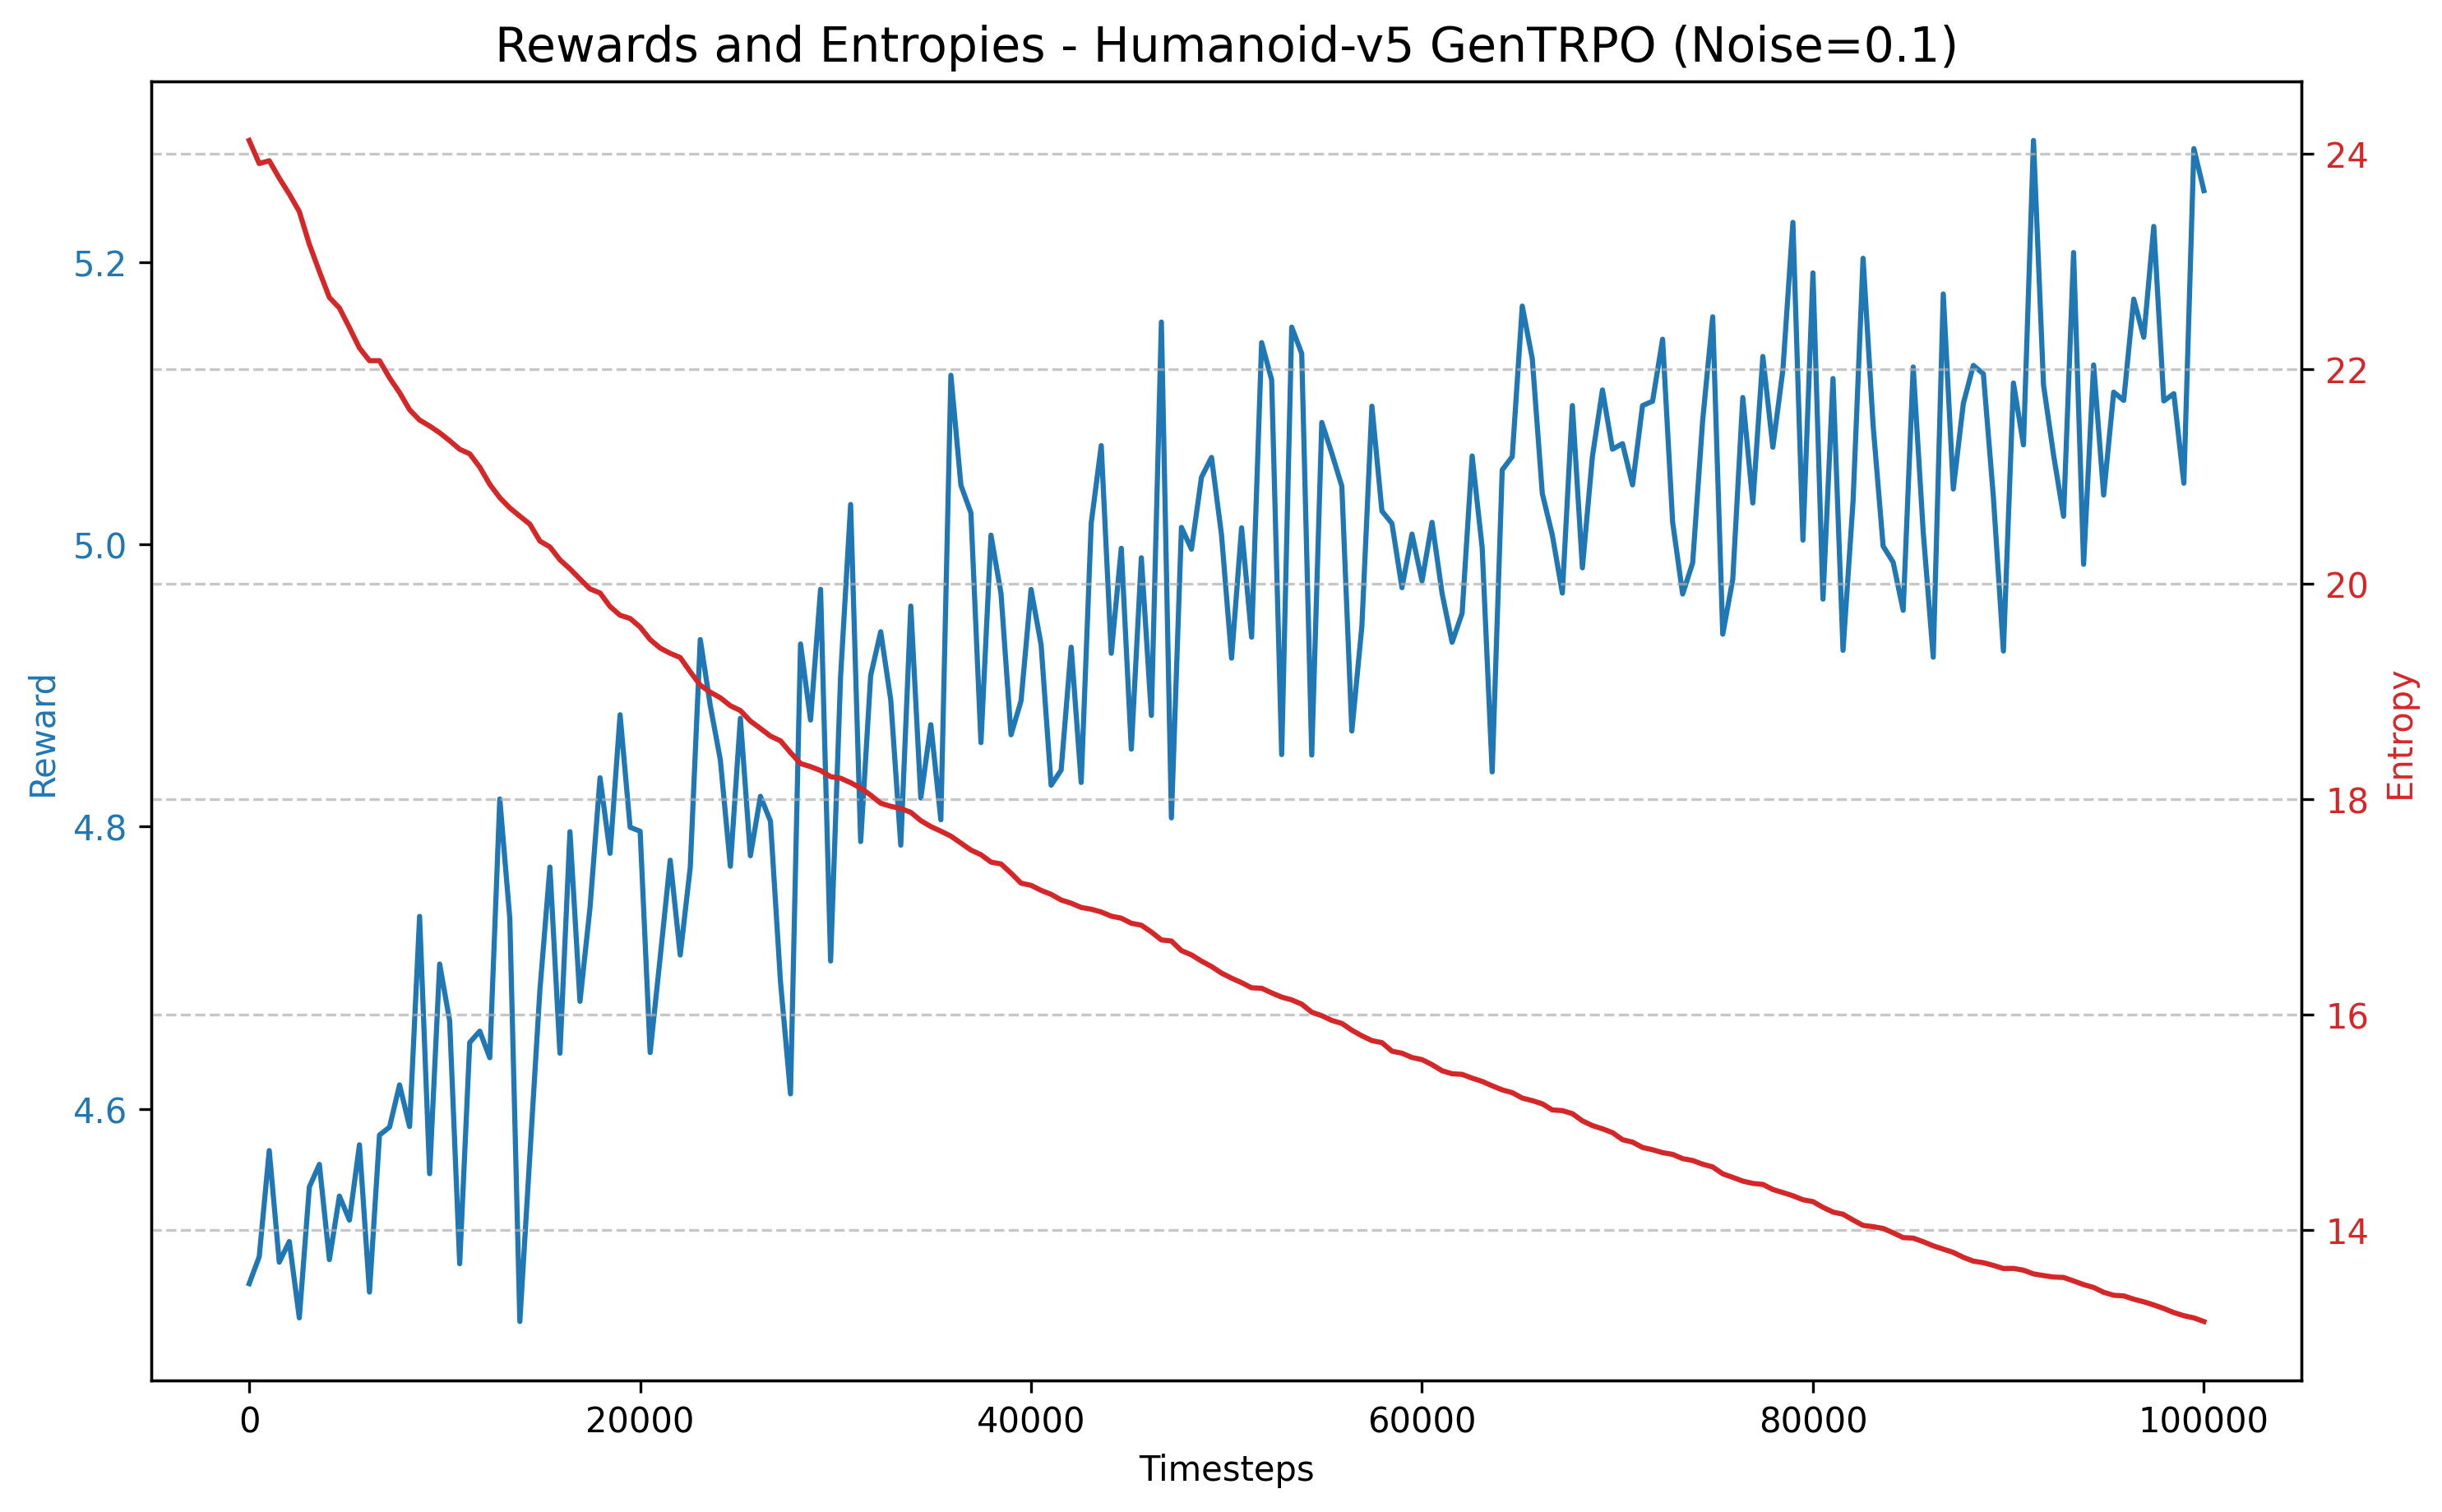
\includegraphics[width=0.8\textwidth]{graph_Humanoid-v5_gentrpo-ne_rewards_entropies.png}
\captionof{figure}{Rewards and entropies over timesteps for GenTRPO in Humanoid-v5.}
\end{center}

The plot for TRPO in HumanoidStandup-v5 shows the reward values (typically on one axis) and entropy values (on another axis) as functions of training timesteps.

\begin{center}
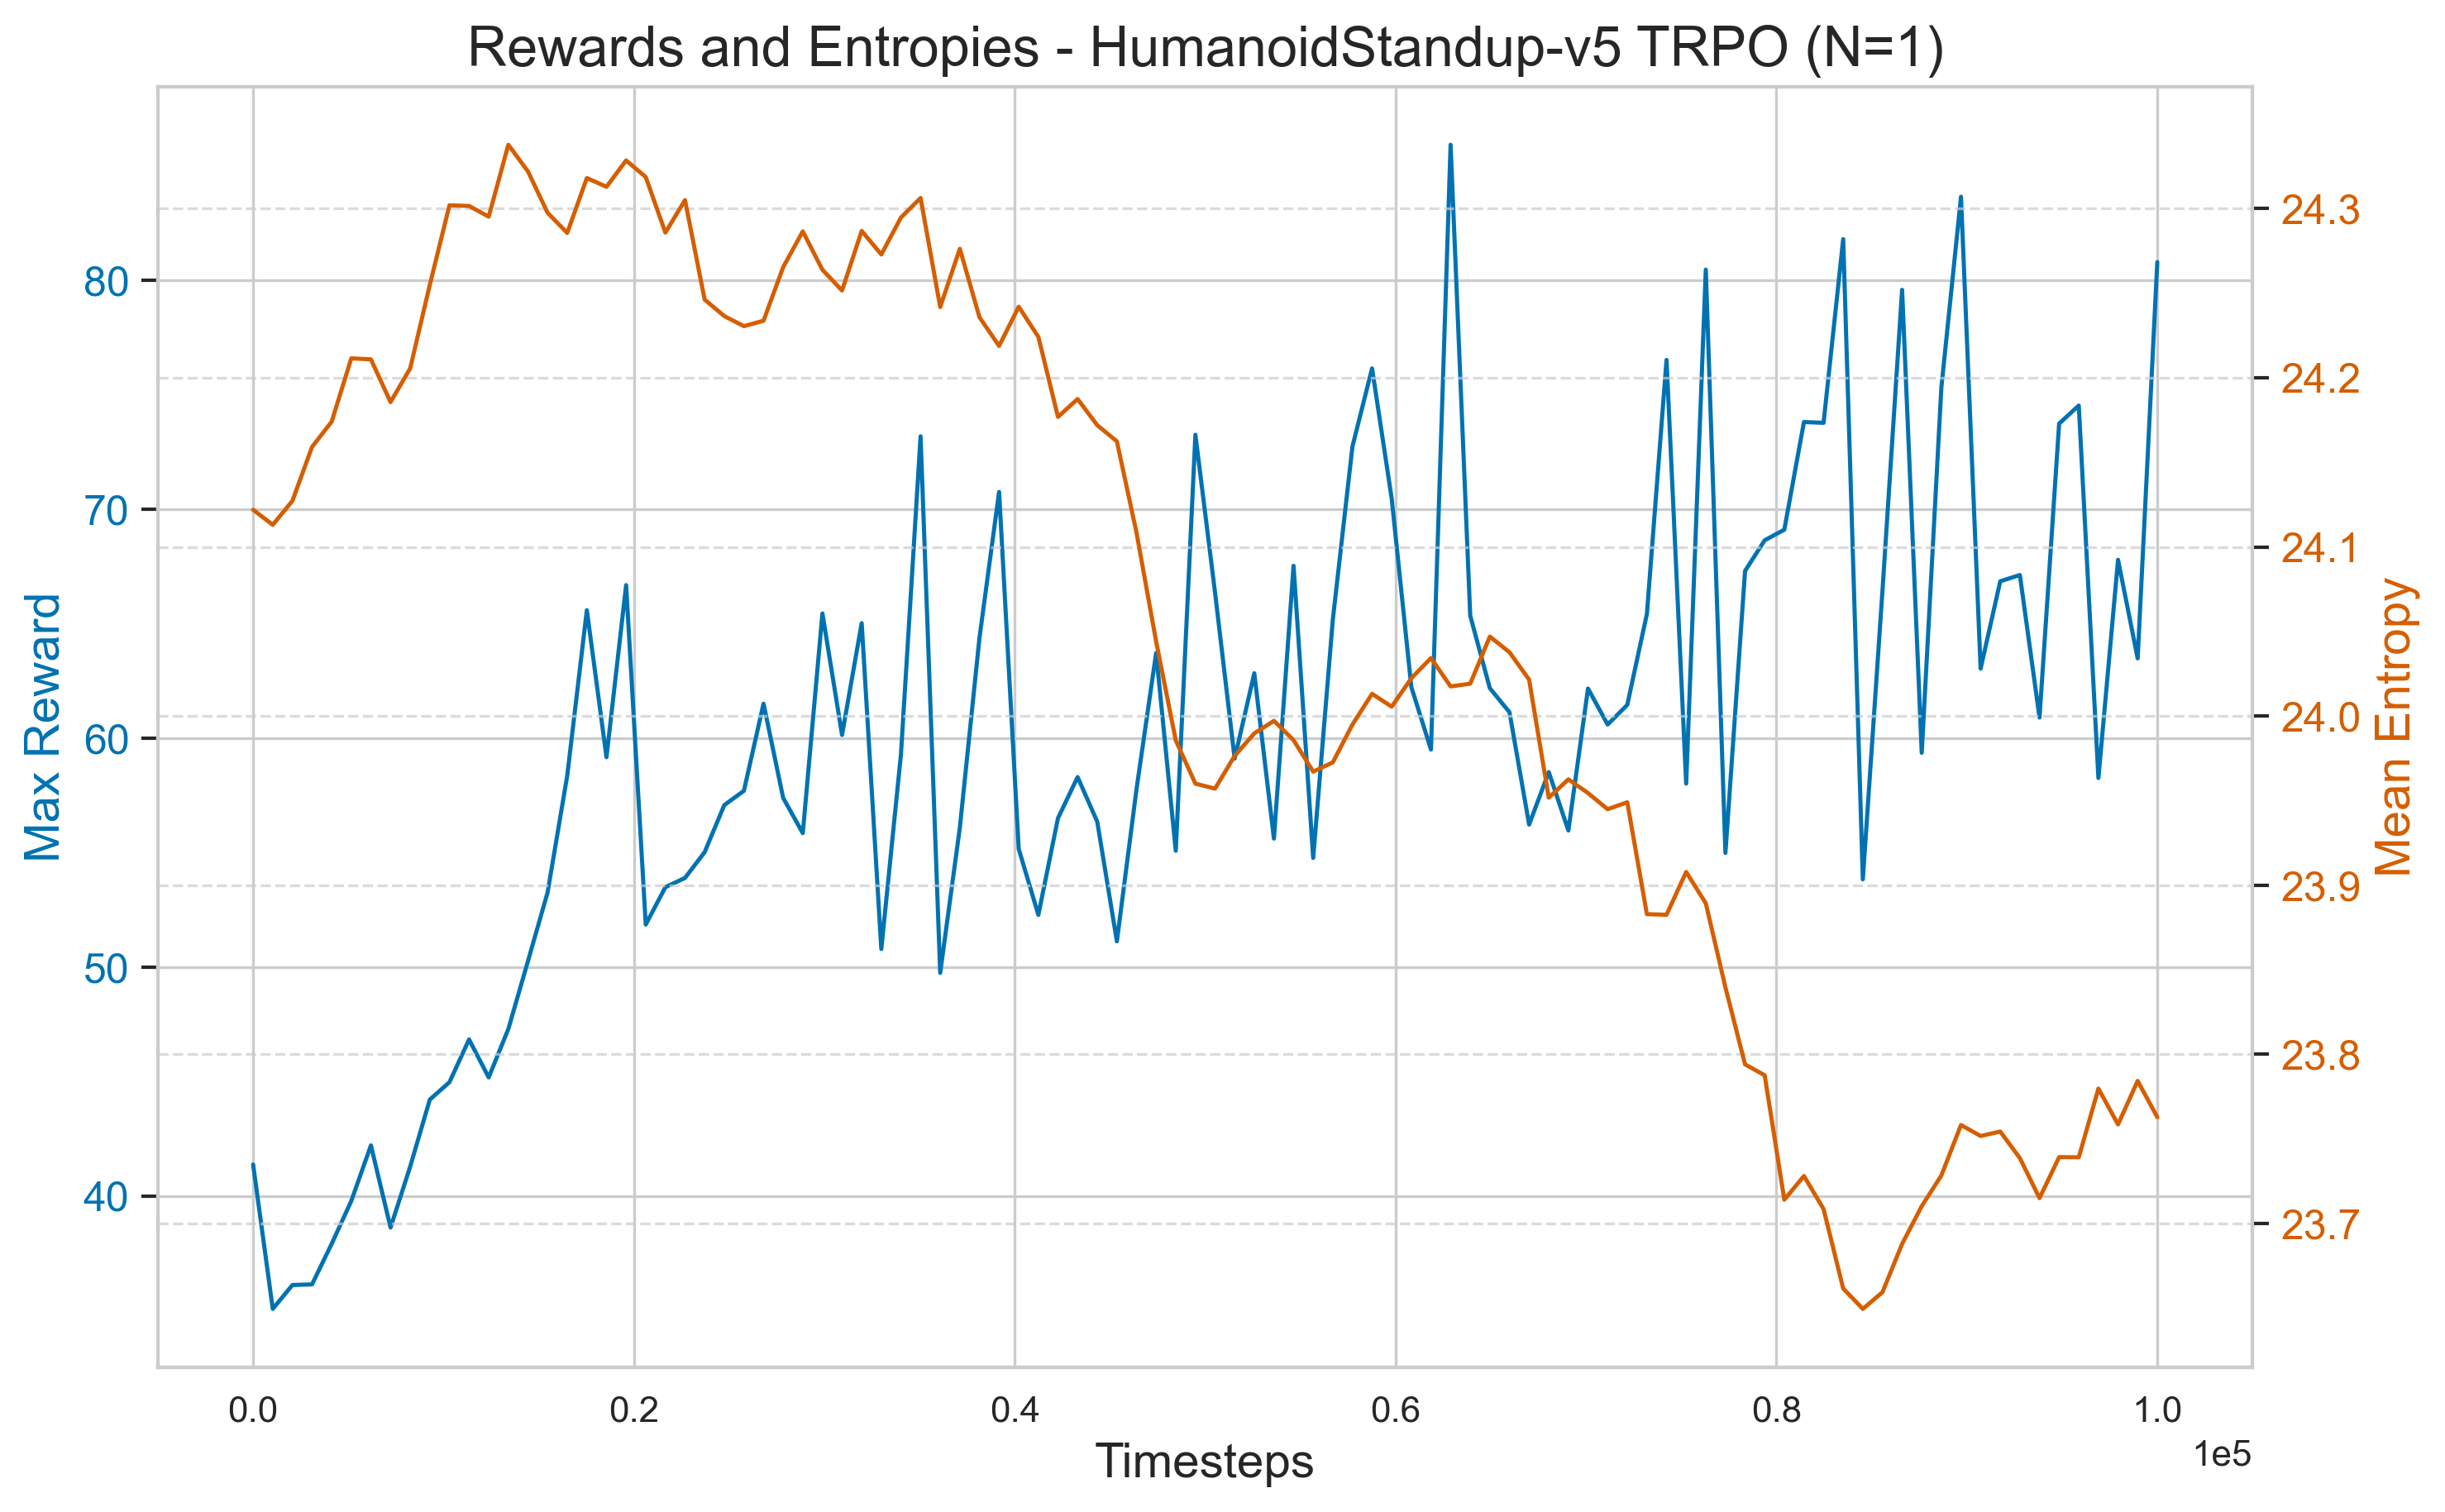
\includegraphics[width=0.8\textwidth]{graph_HumanoidStandup-v5_trpo_rewards_entropies.png}
\captionof{figure}{Rewards and entropies over timesteps for TRPO in HumanoidStandup-v5.}
\end{center}

The plot for GenTRPO (Noise=0) in HumanoidStandup-v5 shows the reward values (typically on one axis) and entropy values (on another axis) as functions of training timesteps.

\begin{center}
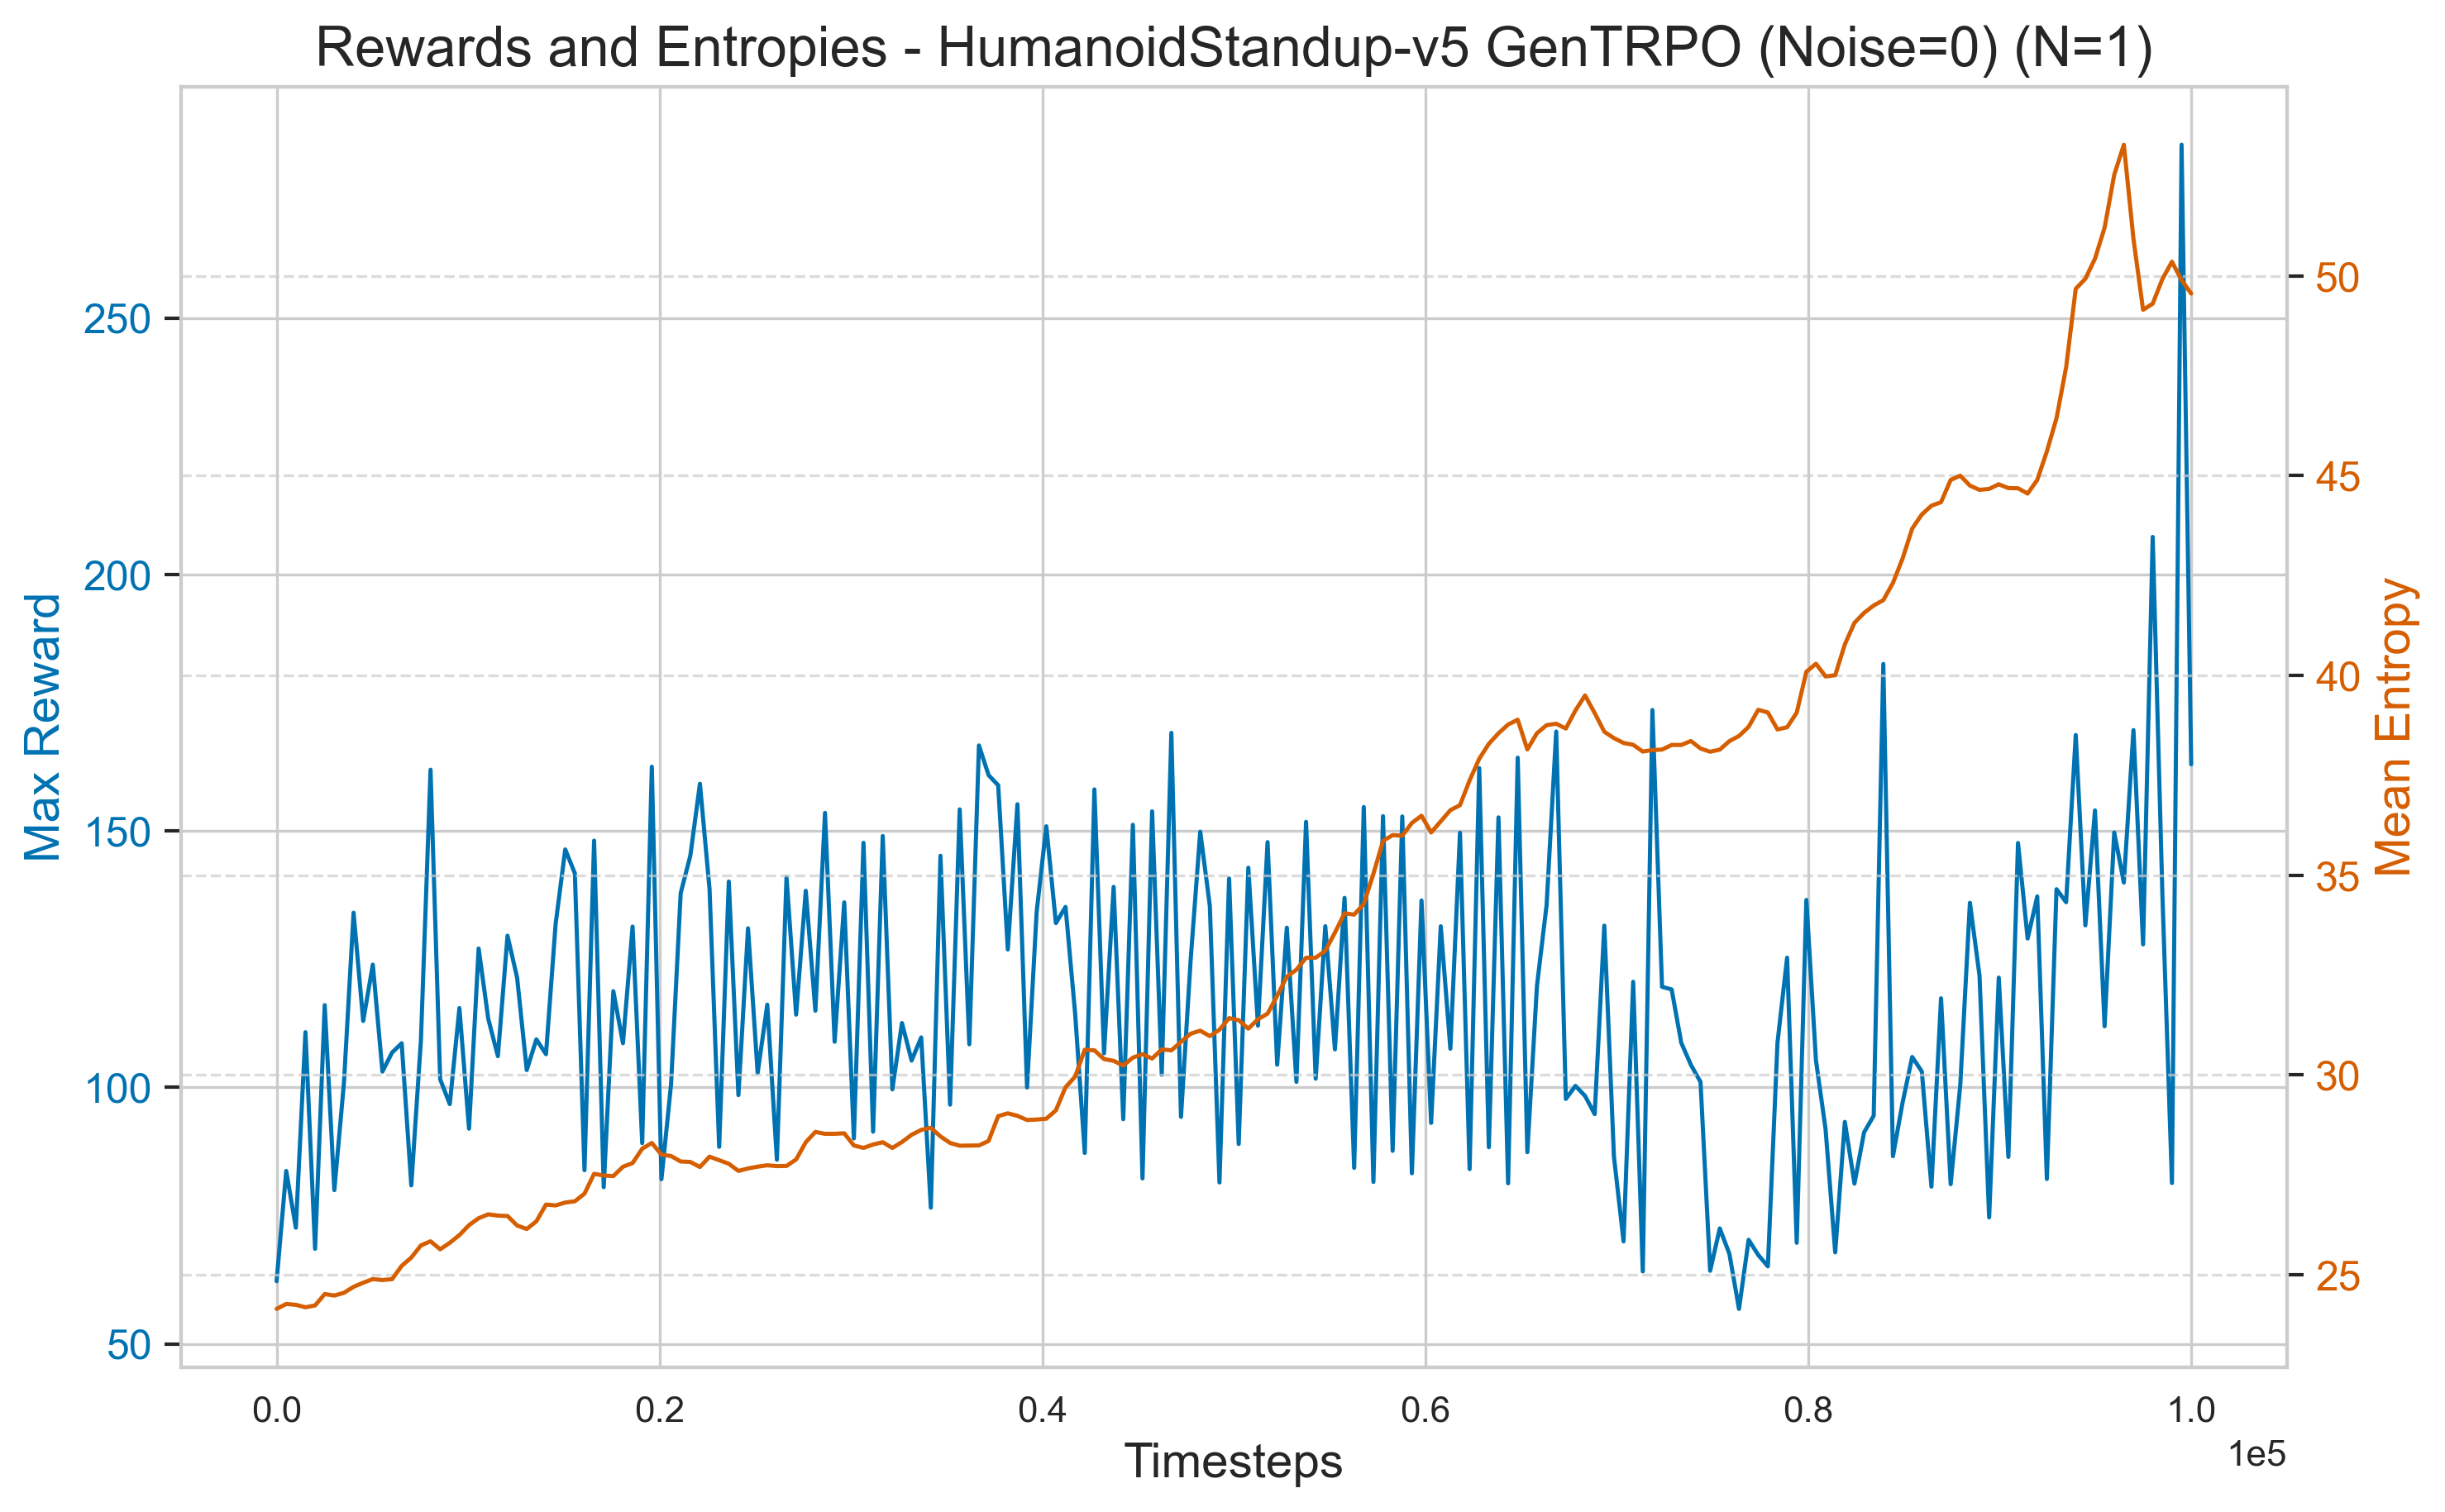
\includegraphics[width=0.8\textwidth]{graph_HumanoidStandup-v5_gentrpo_rewards_entropies.png}
\captionof{figure}{Rewards and entropies over timesteps for GenTRPO (Noise=0) in HumanoidStandup-v5.}
\end{center}

The plot for GenTRPO in HumanoidStandup-v5 shows the reward values (typically on one axis) and entropy values (on another axis) as functions of training timesteps.

\begin{center}
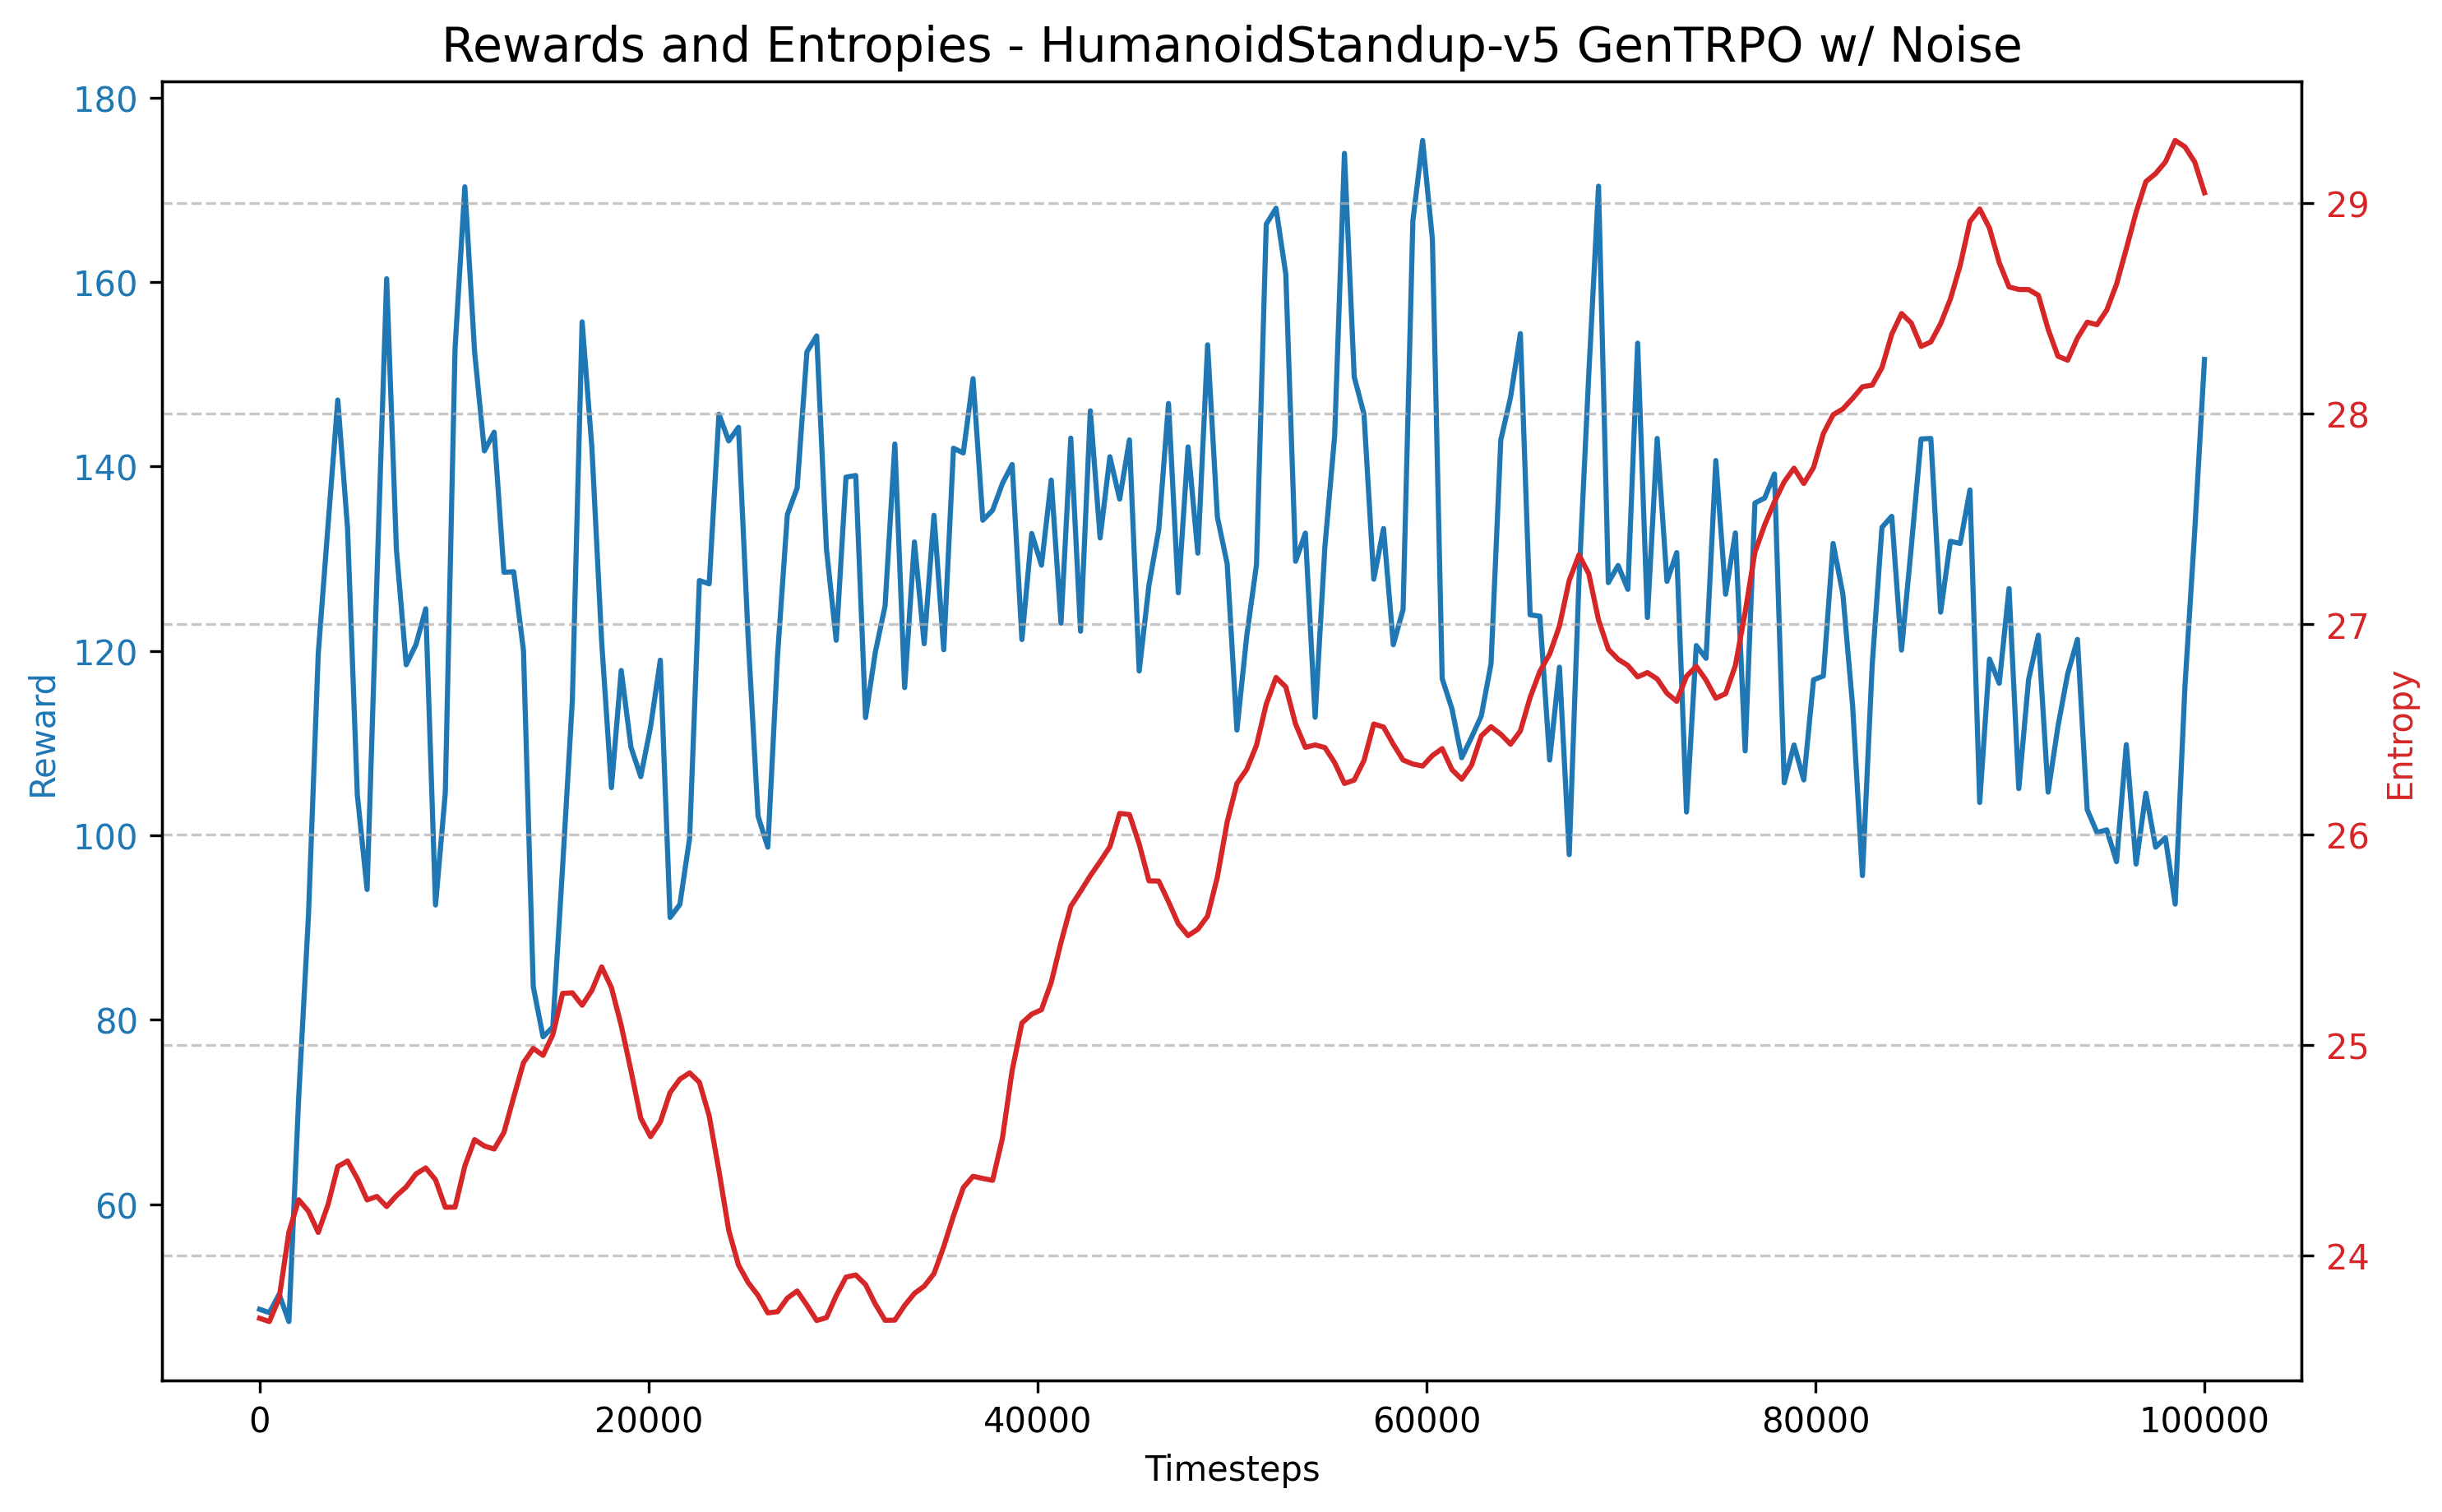
\includegraphics[width=0.8\textwidth]{graph_HumanoidStandup-v5_gentrpo-ne_rewards_entropies.png}
\captionof{figure}{Rewards and entropies over timesteps for GenTRPO in HumanoidStandup-v5.}
\end{center}

\subsection{Comparative Rewards Plots}
These plots compare the reward curves across all models for a specific environment. They allow for visual comparison of how different models perform in terms of rewards over the training period.

The comparative rewards plot for Humanoid-v5 aggregates the reward curves from all models, enabling side-by-side evaluation.

\begin{center}
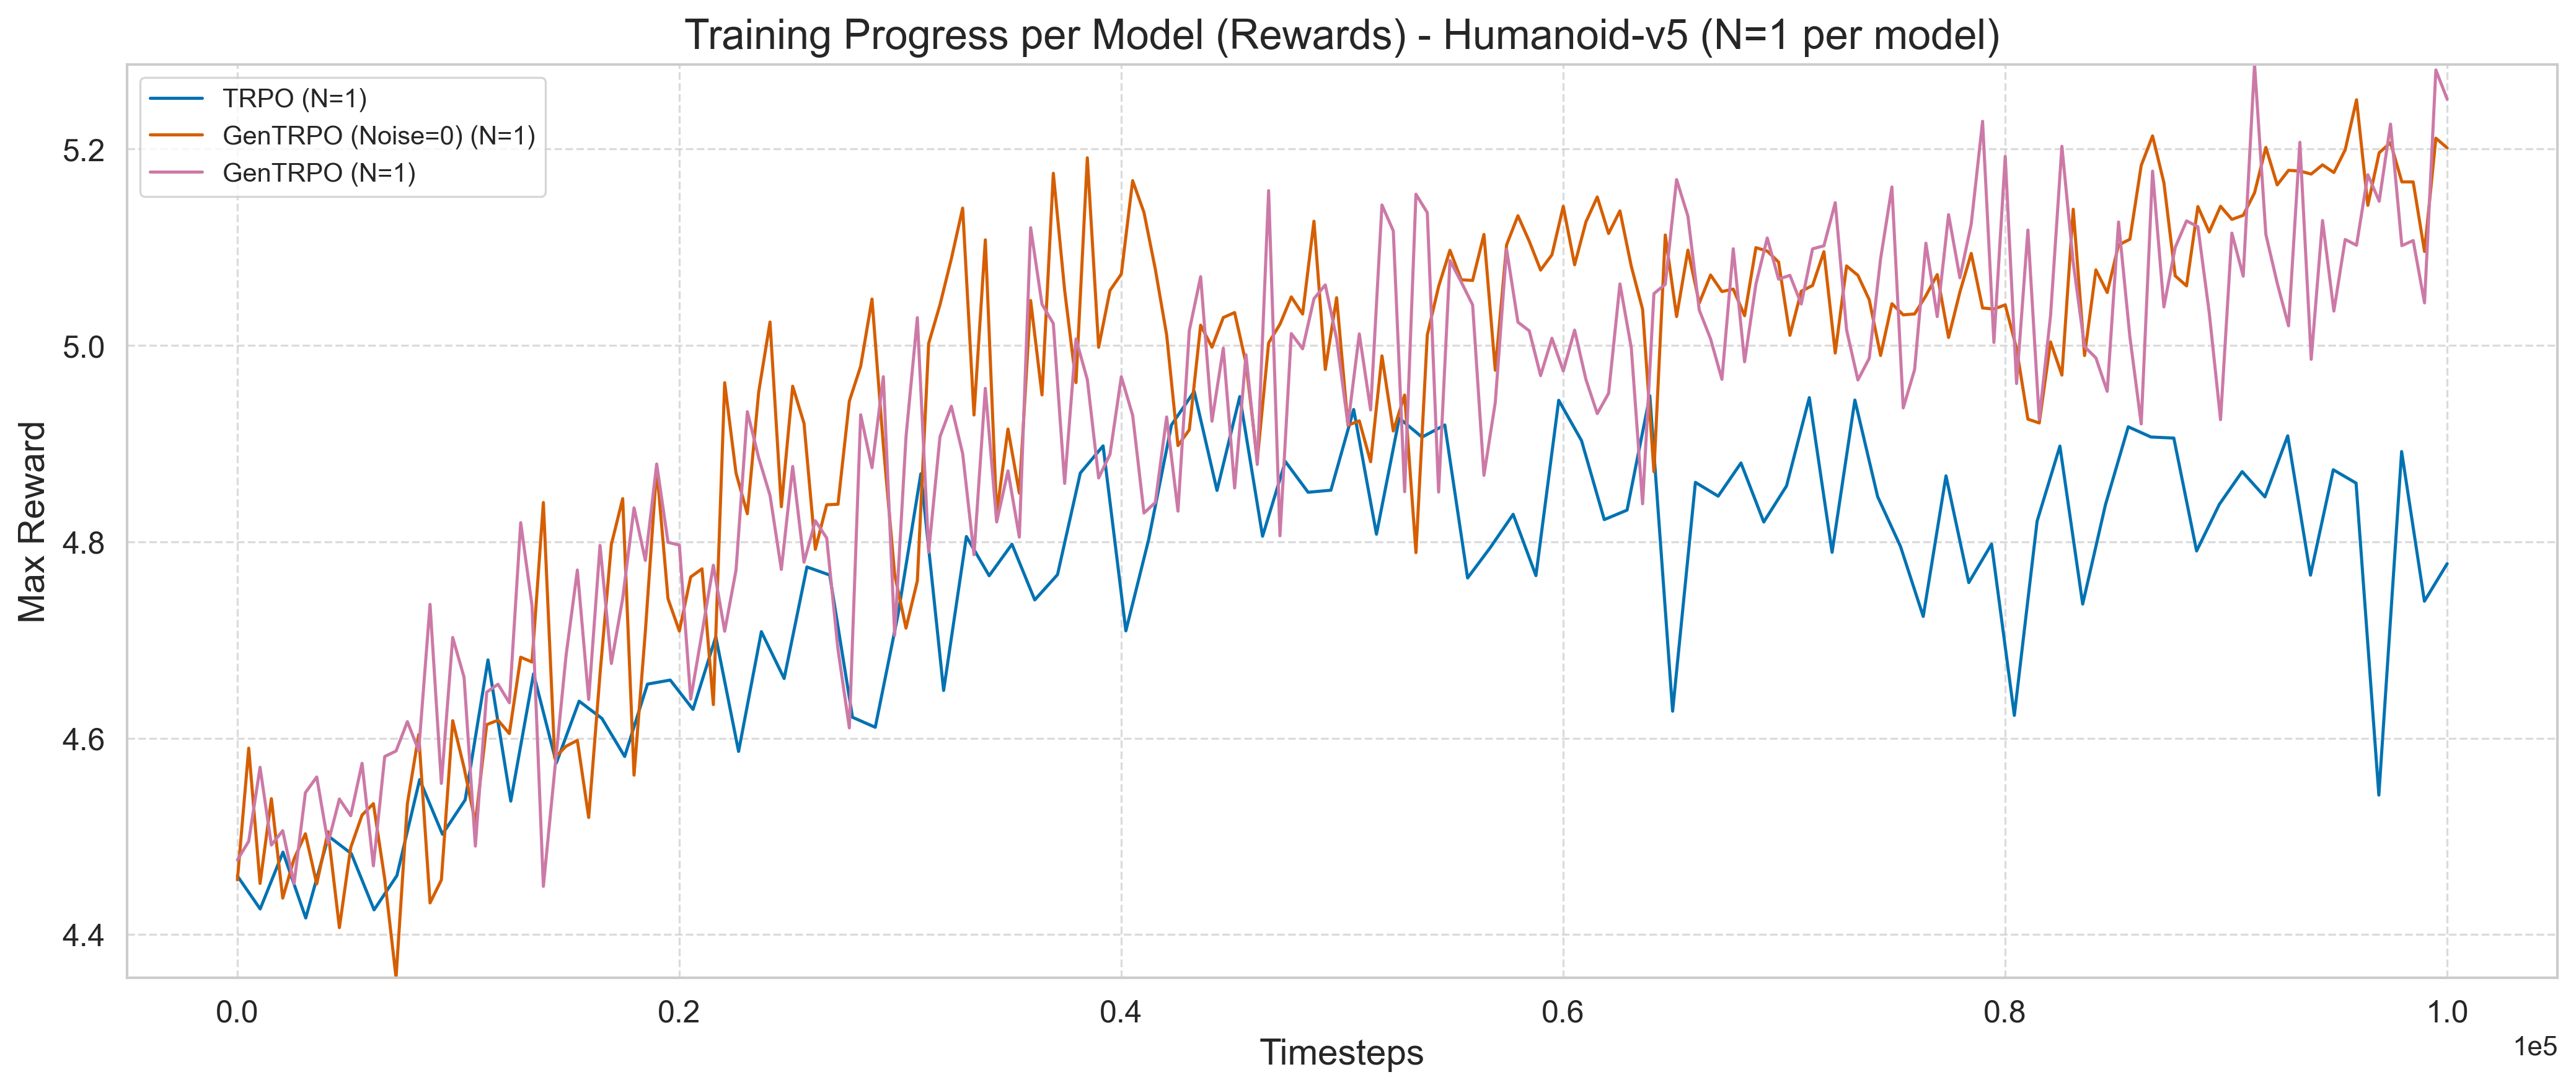
\includegraphics[width=0.8\textwidth]{graph_Humanoid-v5_models_rewards.png}
\captionof{figure}{Comparative rewards over timesteps across all models in Humanoid-v5.}
\end{center}

The comparative rewards plot for HumanoidStandup-v5 aggregates the reward curves from all models, enabling side-by-side evaluation.

\begin{center}
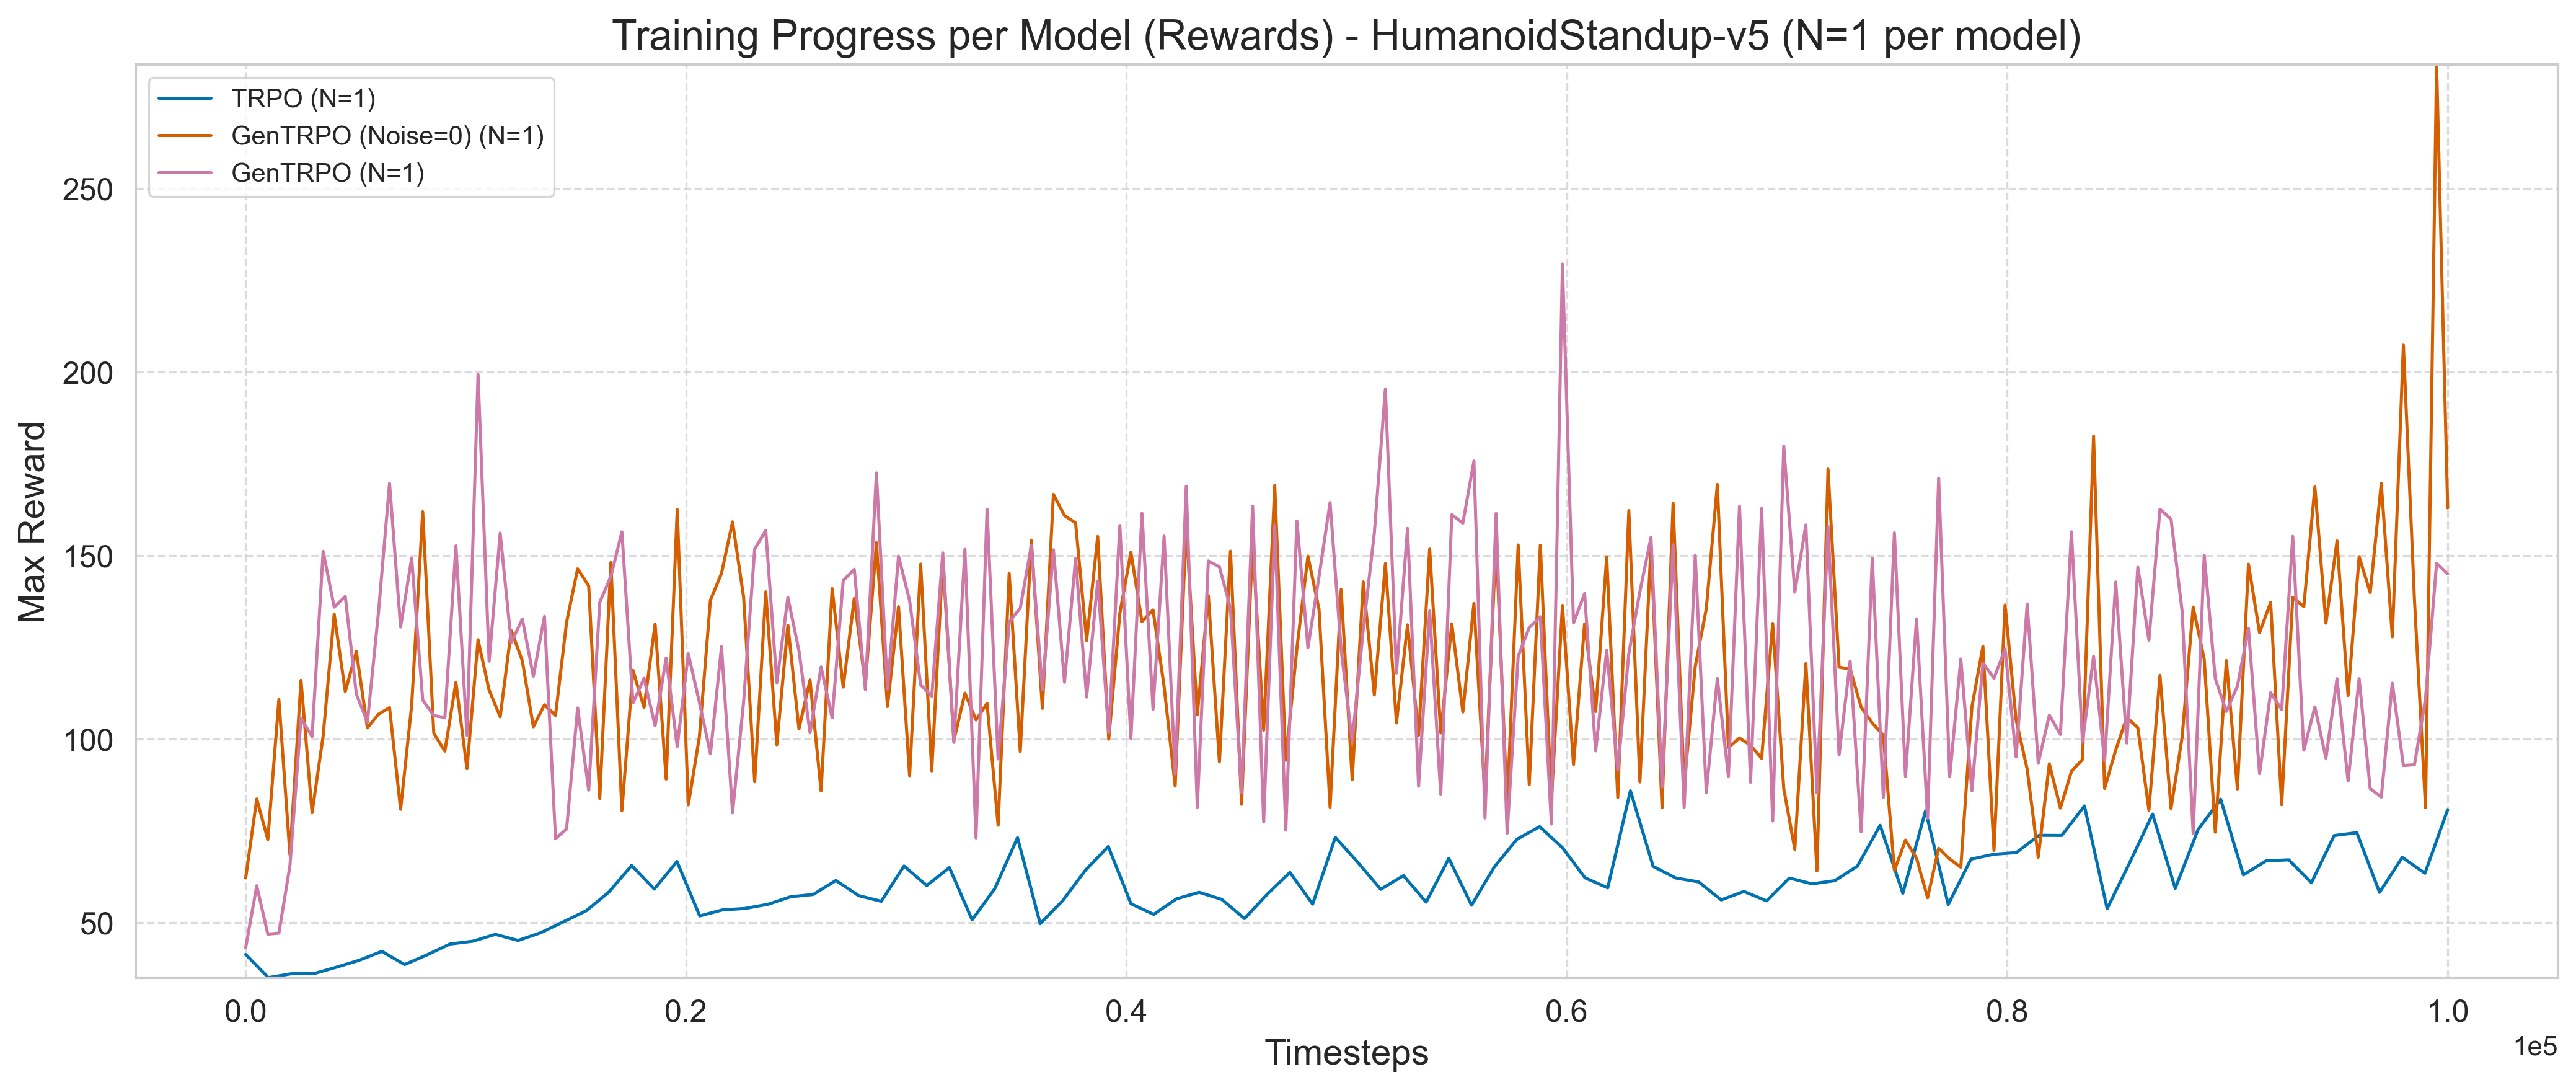
\includegraphics[width=0.8\textwidth]{graph_HumanoidStandup-v5_models_rewards.png}
\captionof{figure}{Comparative rewards over timesteps across all models in HumanoidStandup-v5.}
\end{center}

\subsection{Comparative Entropies Plots}
Similar to the comparative rewards, these plots show the entropy curves across all models for each environment, highlighting differences in exploration behavior.

The comparative entropies plot for Humanoid-v5 aggregates the entropy curves from all models.

\begin{center}
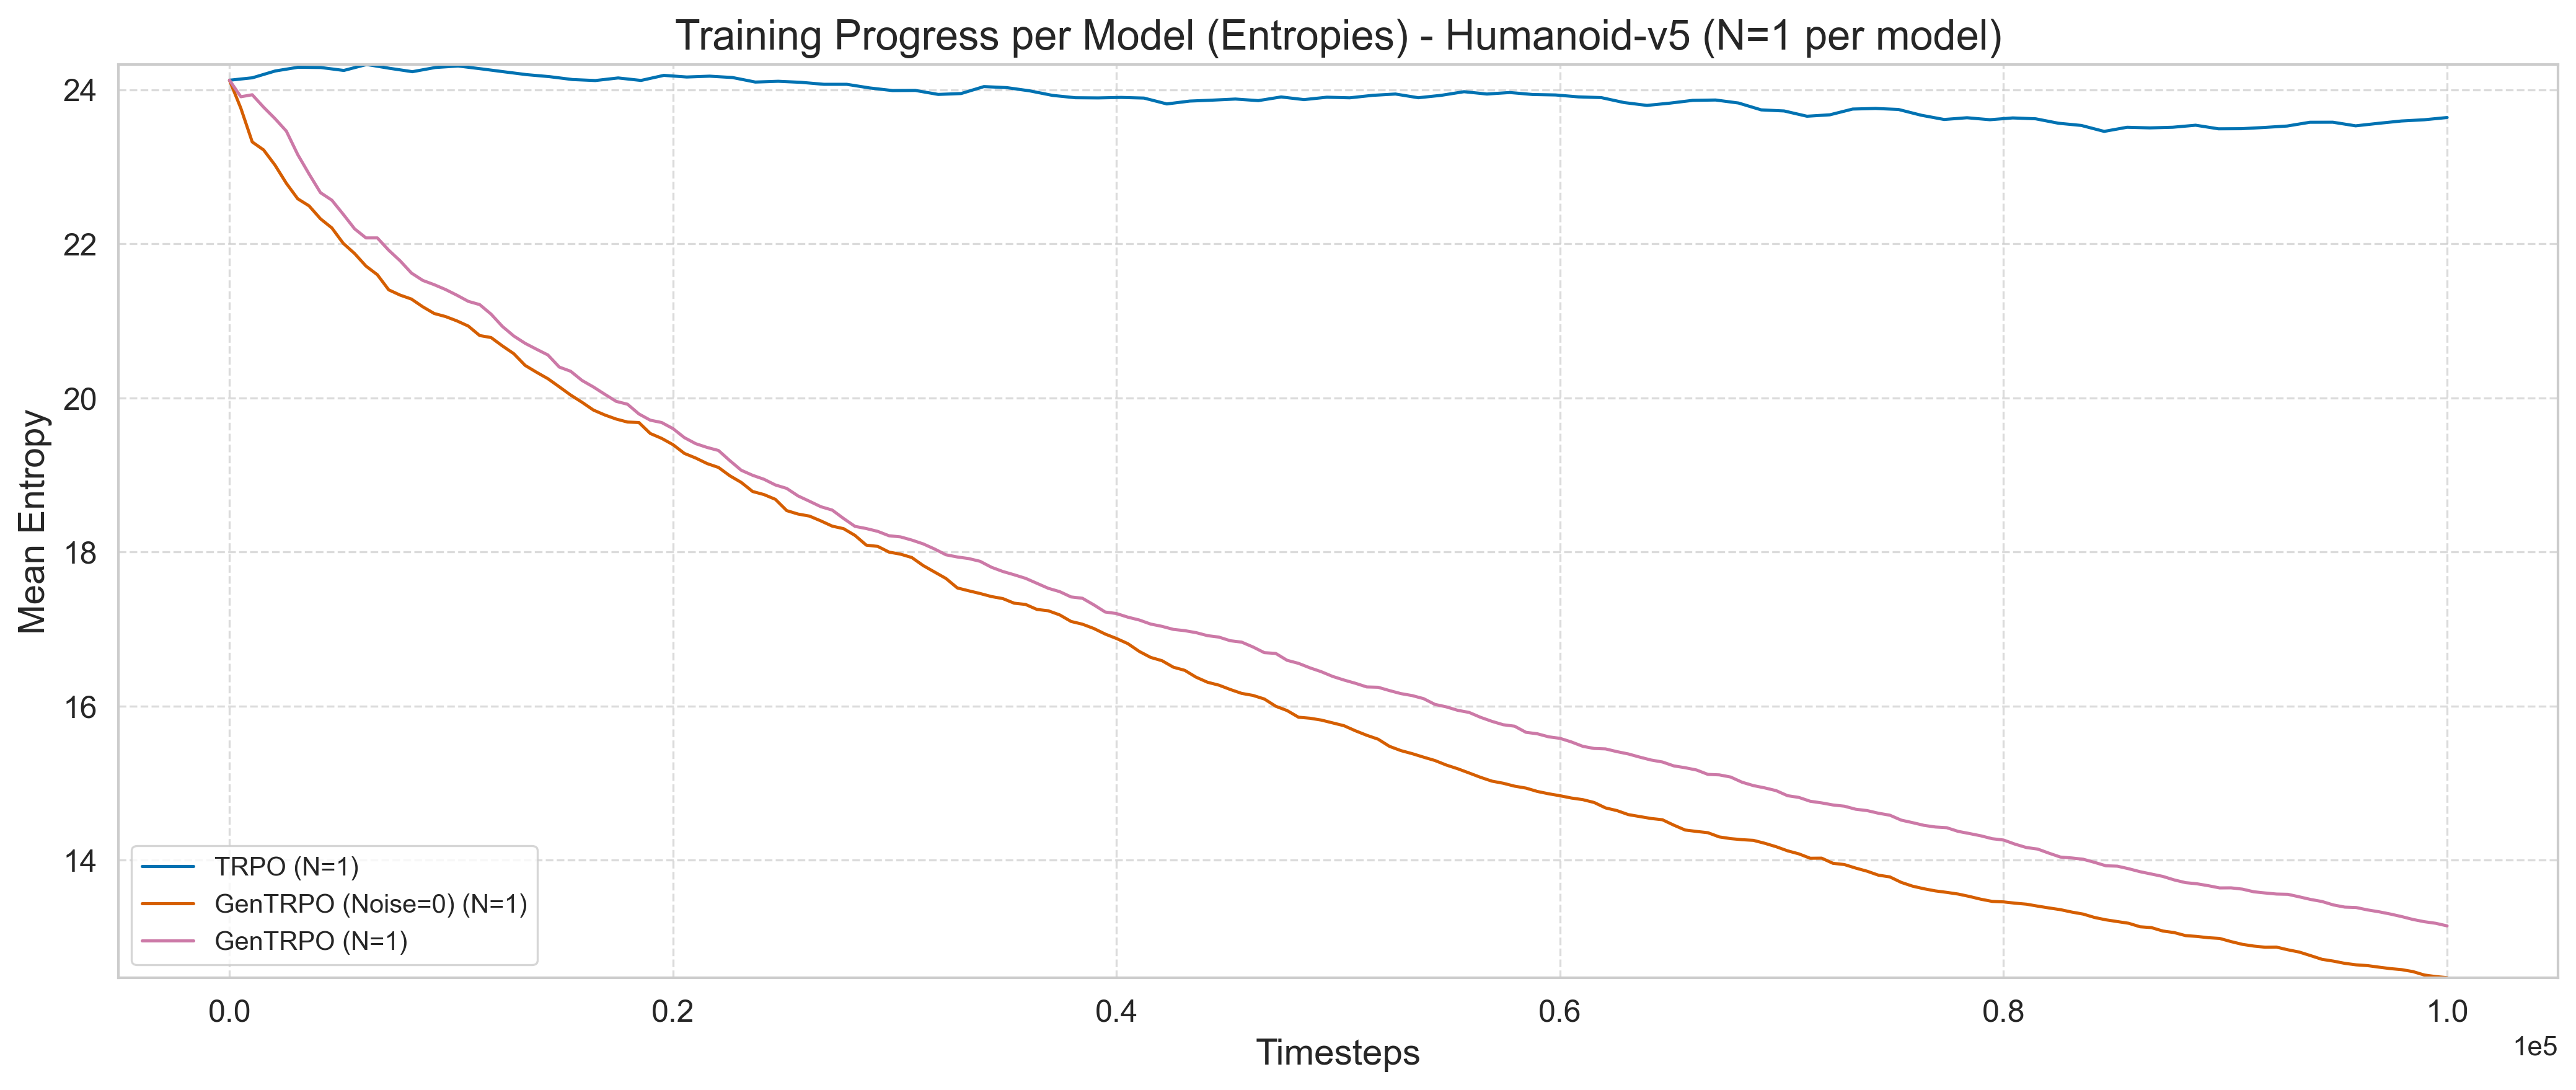
\includegraphics[width=0.8\textwidth]{graph_Humanoid-v5_models_entropies.png}
\captionof{figure}{Comparative entropies over timesteps across all models in Humanoid-v5.}
\end{center}

The comparative entropies plot for HumanoidStandup-v5 aggregates the entropy curves from all models.

\begin{center}
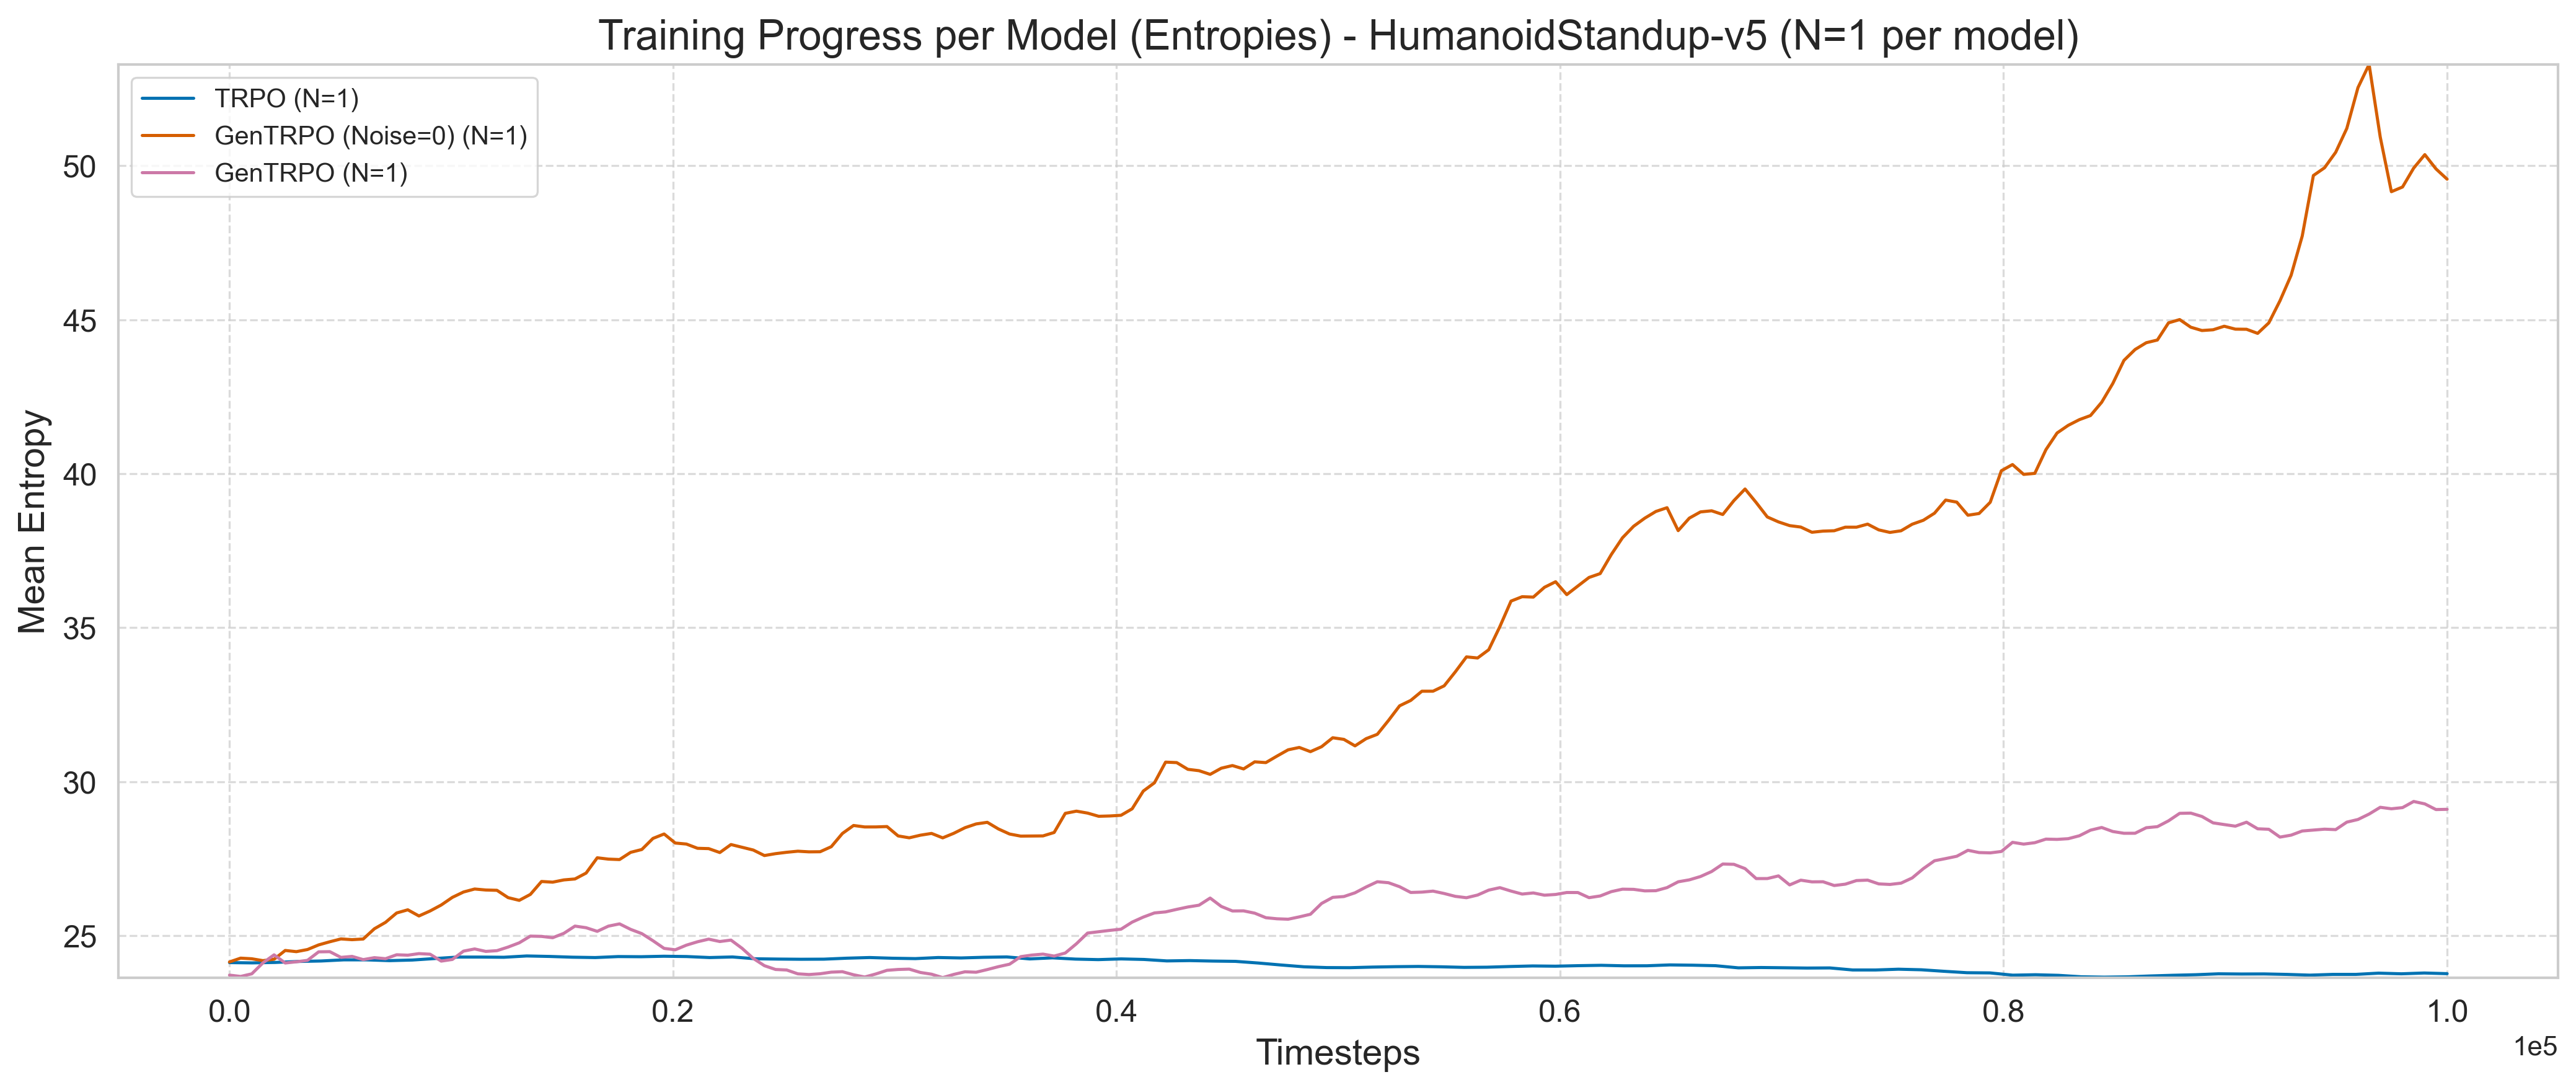
\includegraphics[width=0.8\textwidth]{graph_HumanoidStandup-v5_models_entropies.png}
\captionof{figure}{Comparative entropies over timesteps across all models in HumanoidStandup-v5.}
\end{center}

\subsection{Noise Modulation Grid Plots}
These grid plots show the rewards and entropies across different noise levels for GenTRPO and TRPO in each environment.

The grid plot for GenTRPO rewards across noise levels in Humanoid-v5.

\begin{center}
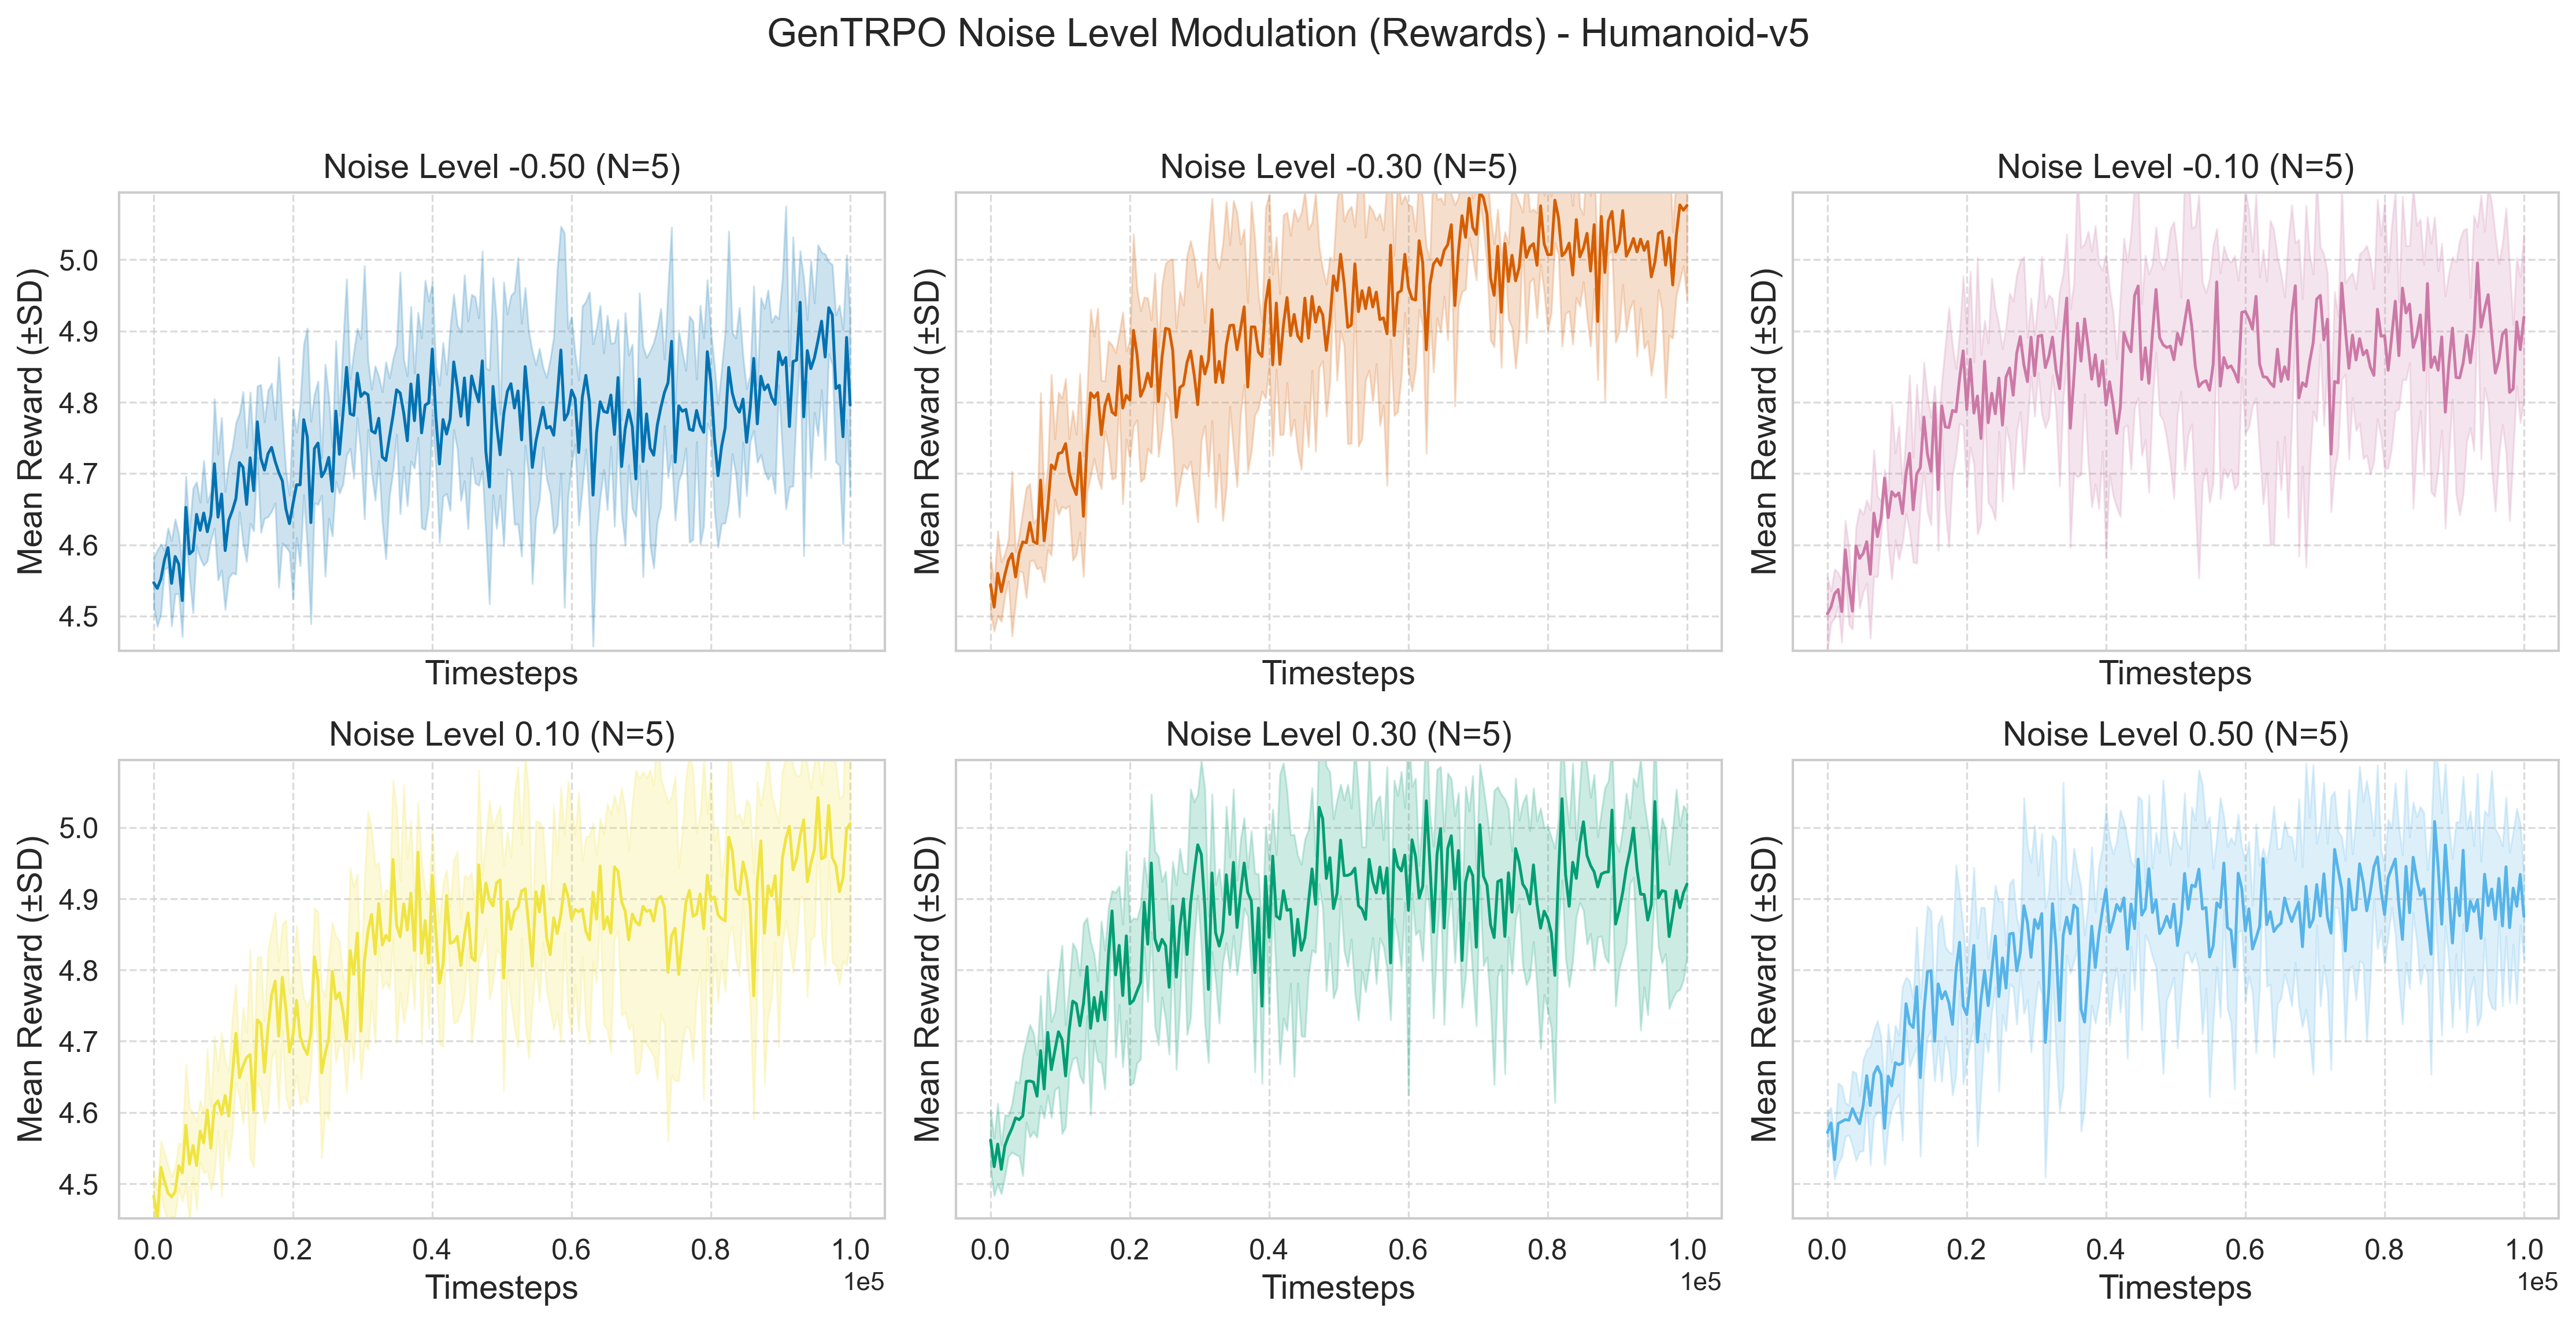
\includegraphics[width=0.8\textwidth]{graph_Humanoid-v5_GenTRPO_noise_mod_rewards_grid.png}
\captionof{figure}{Noise modulation grid for rewards in GenTRPO for Humanoid-v5.}
\end{center}

The grid plot for GenTRPO entropies across noise levels in Humanoid-v5.

\begin{center}
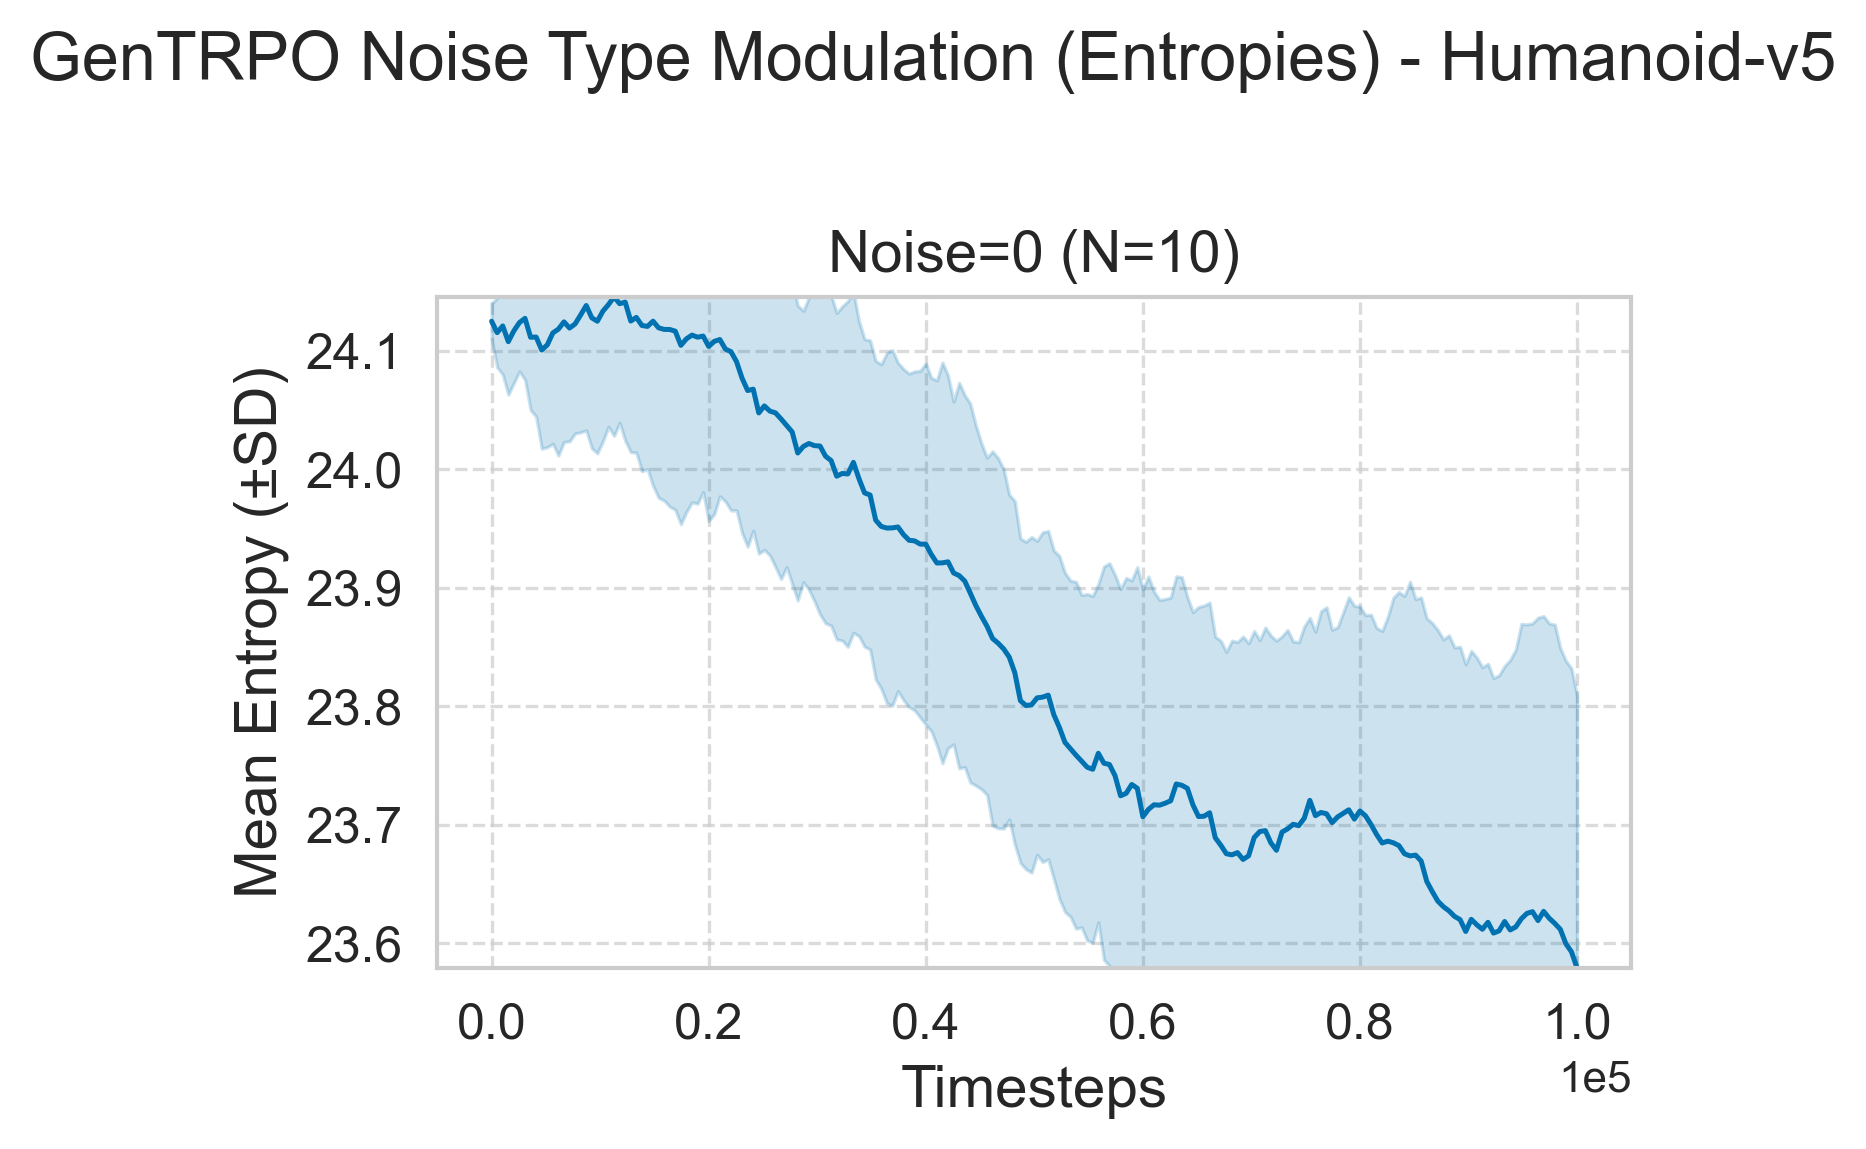
\includegraphics[width=0.8\textwidth]{graph_Humanoid-v5_GenTRPO_noise_mod_entropies_grid.png}
\captionof{figure}{Noise modulation grid for entropies in GenTRPO for Humanoid-v5.}
\end{center}

The grid plot for TRPO rewards across noise levels in Humanoid-v5.

\begin{center}
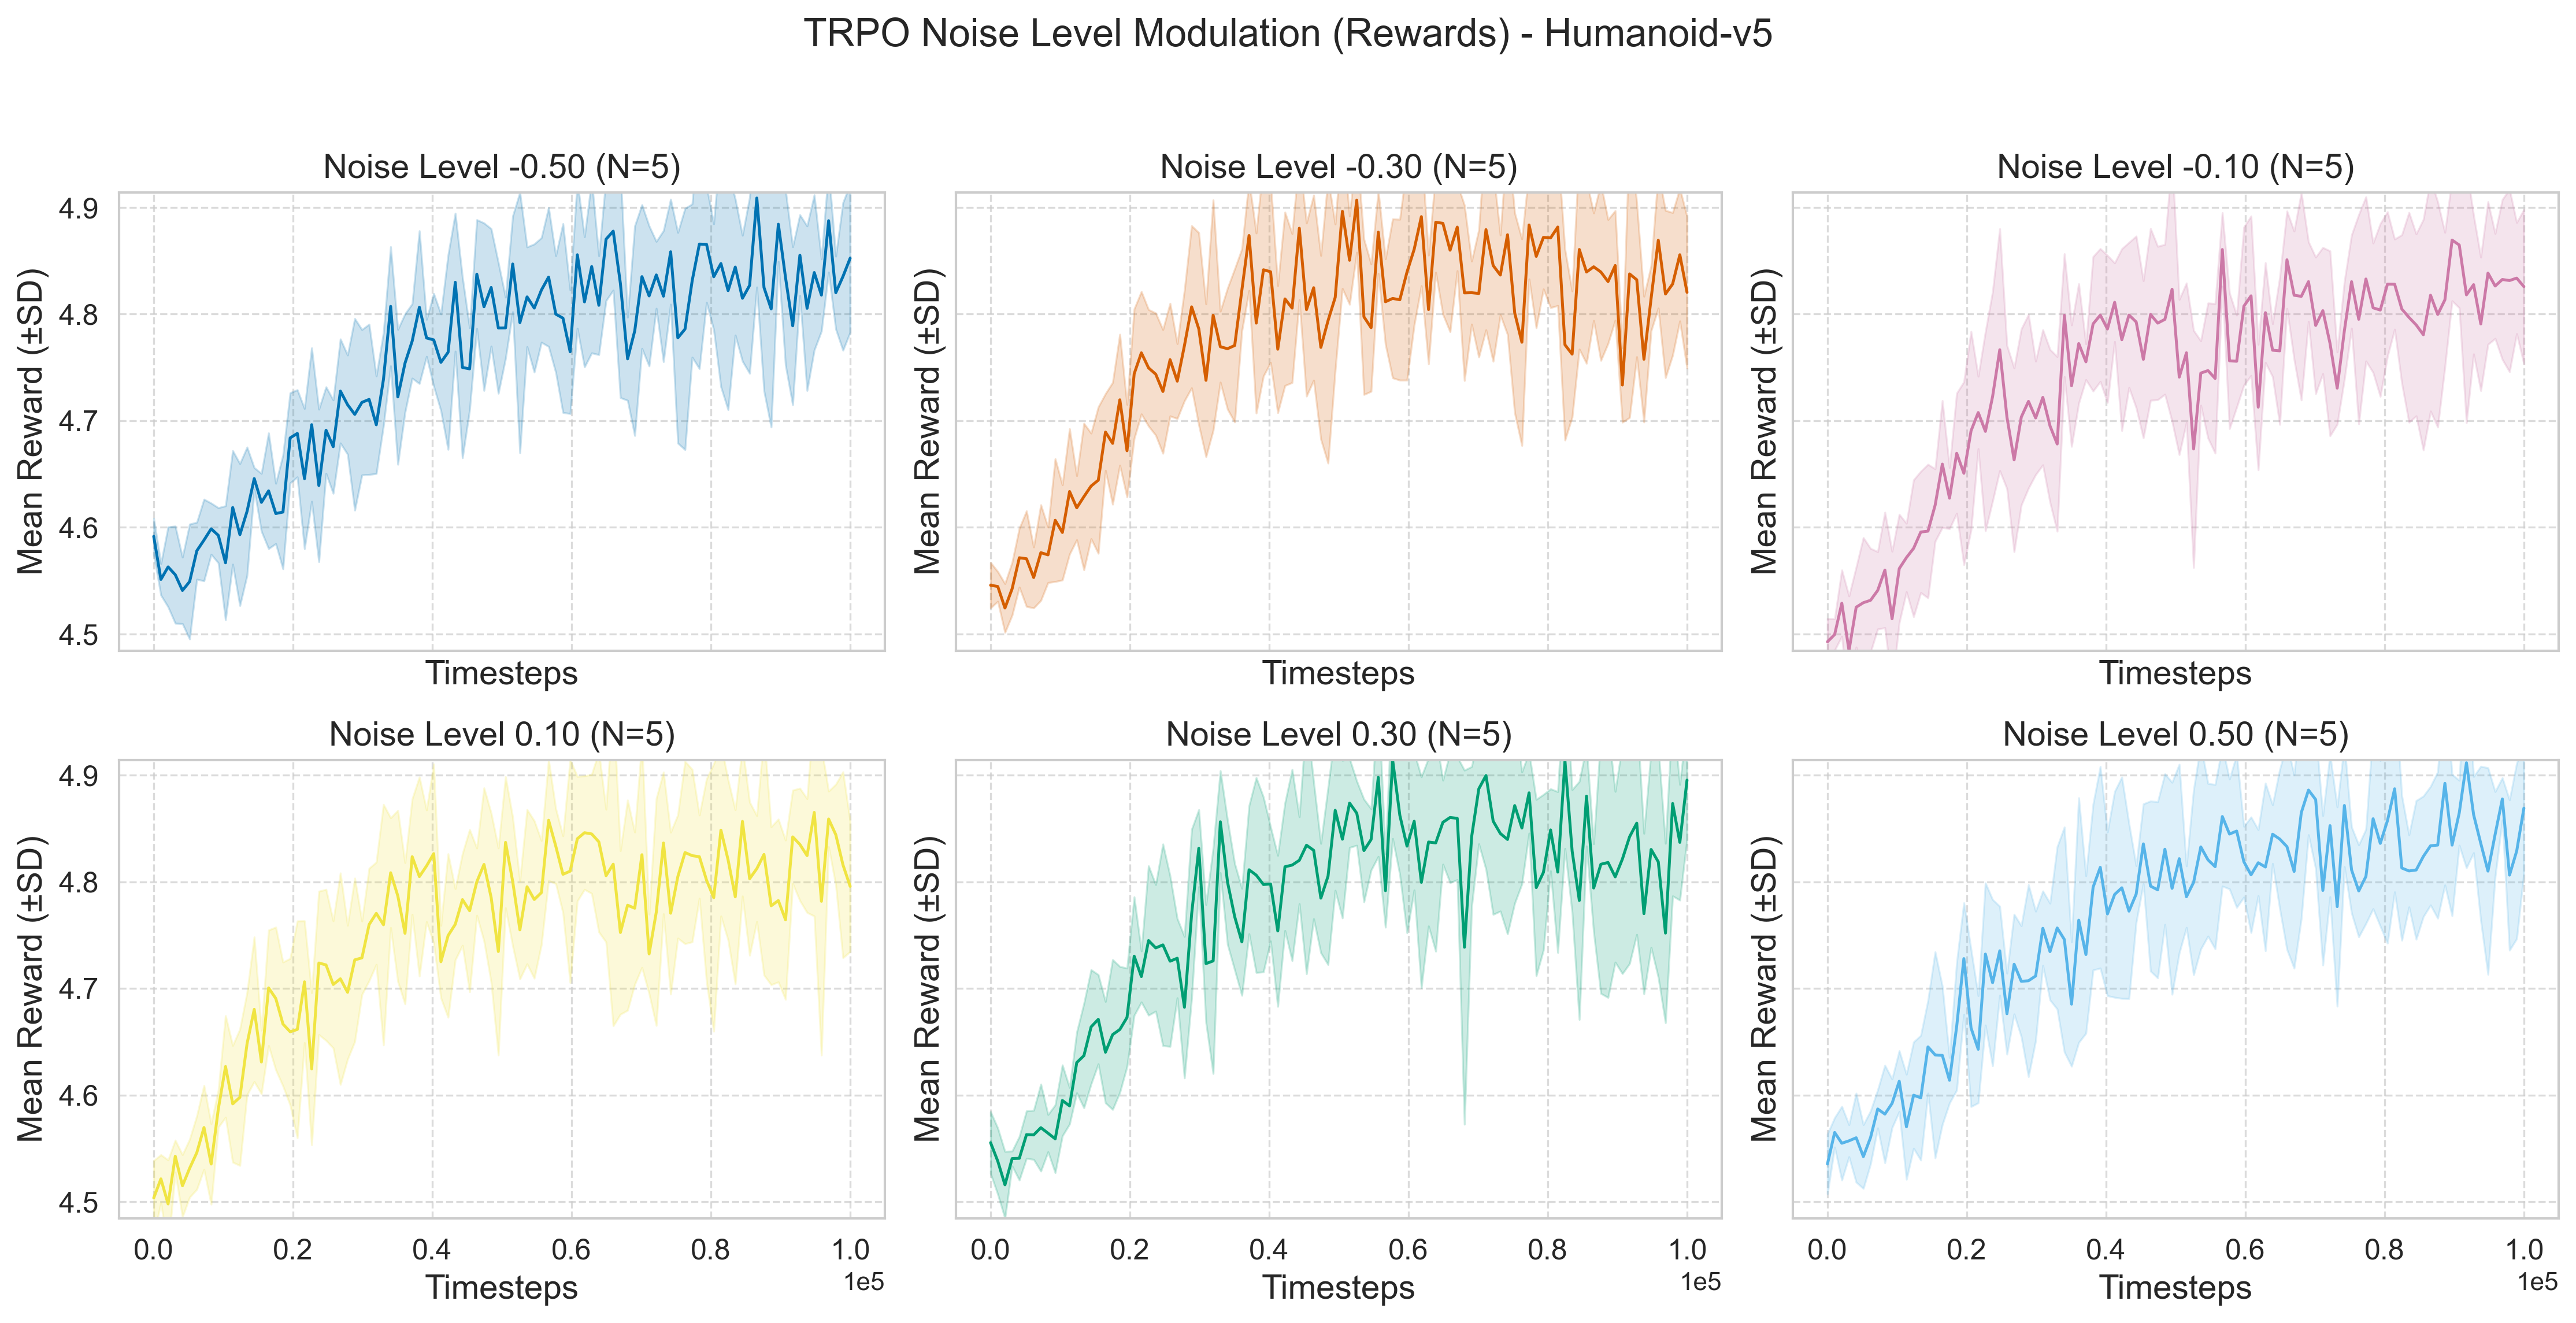
\includegraphics[width=0.8\textwidth]{graph_Humanoid-v5_TRPO_noise_mod_rewards_grid.png}
\captionof{figure}{Noise modulation grid for rewards in TRPO for Humanoid-v5.}
\end{center}

The grid plot for TRPO entropies across noise levels in Humanoid-v5.

\begin{center}
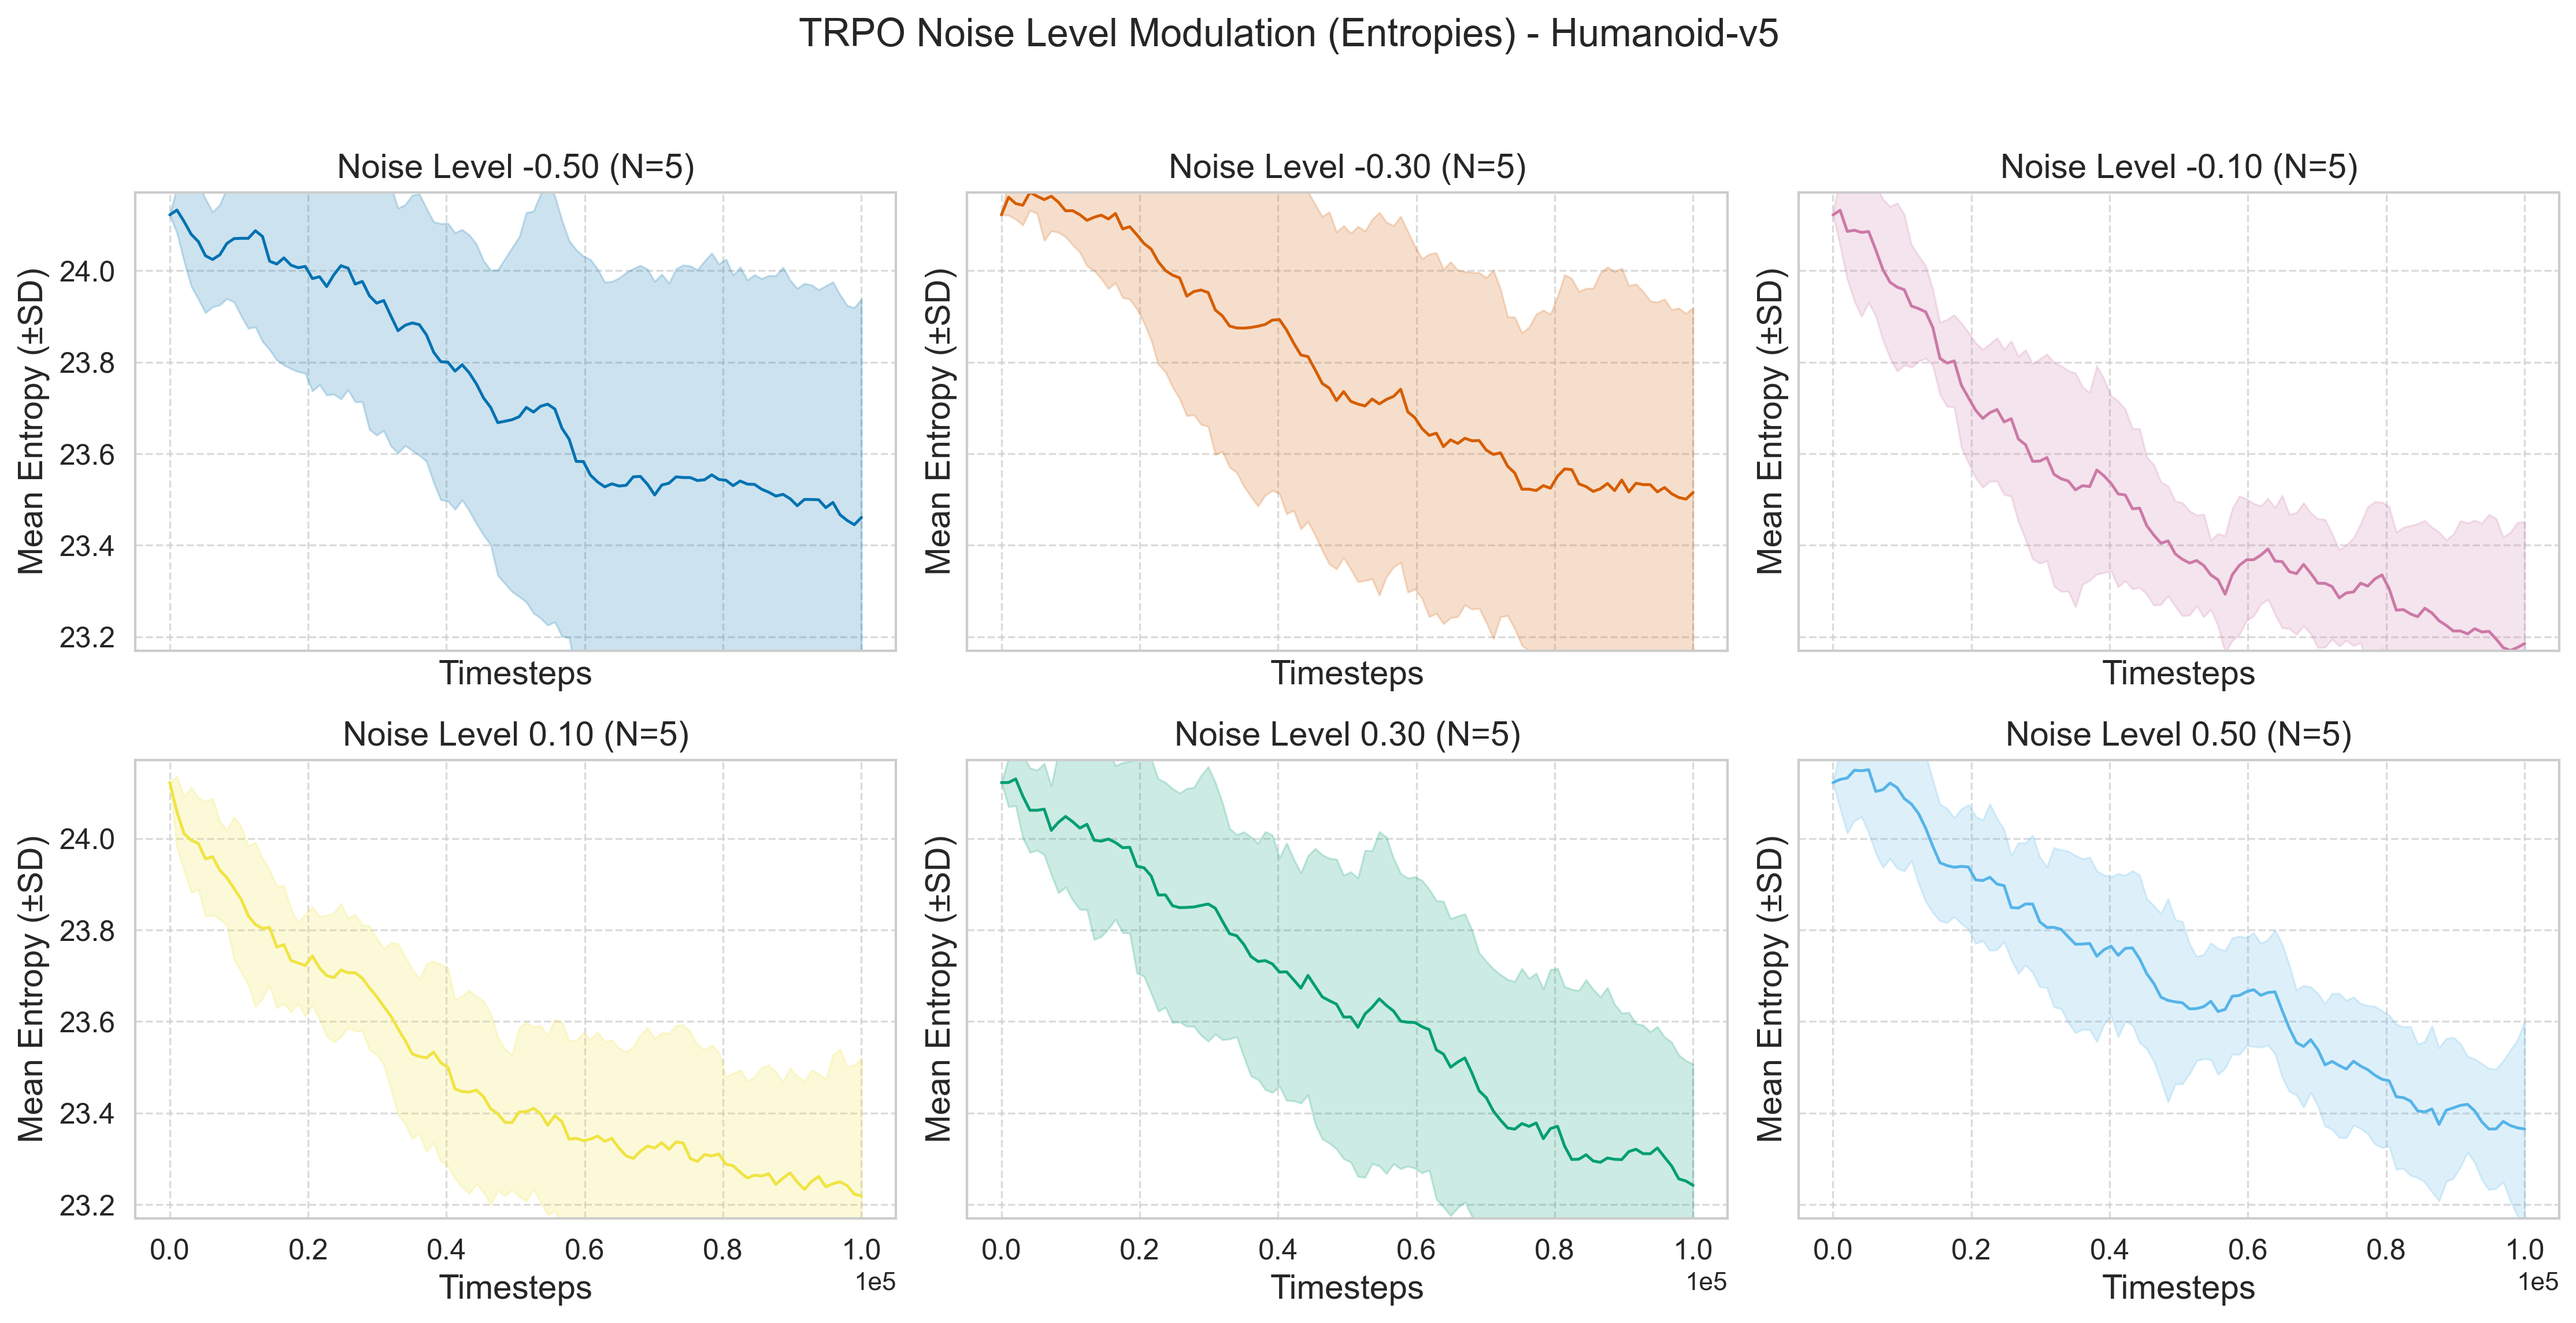
\includegraphics[width=0.8\textwidth]{graph_Humanoid-v5_TRPO_noise_mod_entropies_grid.png}
\captionof{figure}{Noise modulation grid for entropies in TRPO for Humanoid-v5.}
\end{center}

The grid plot for GenTRPO rewards across noise levels in HumanoidStandup-v5.

\begin{center}
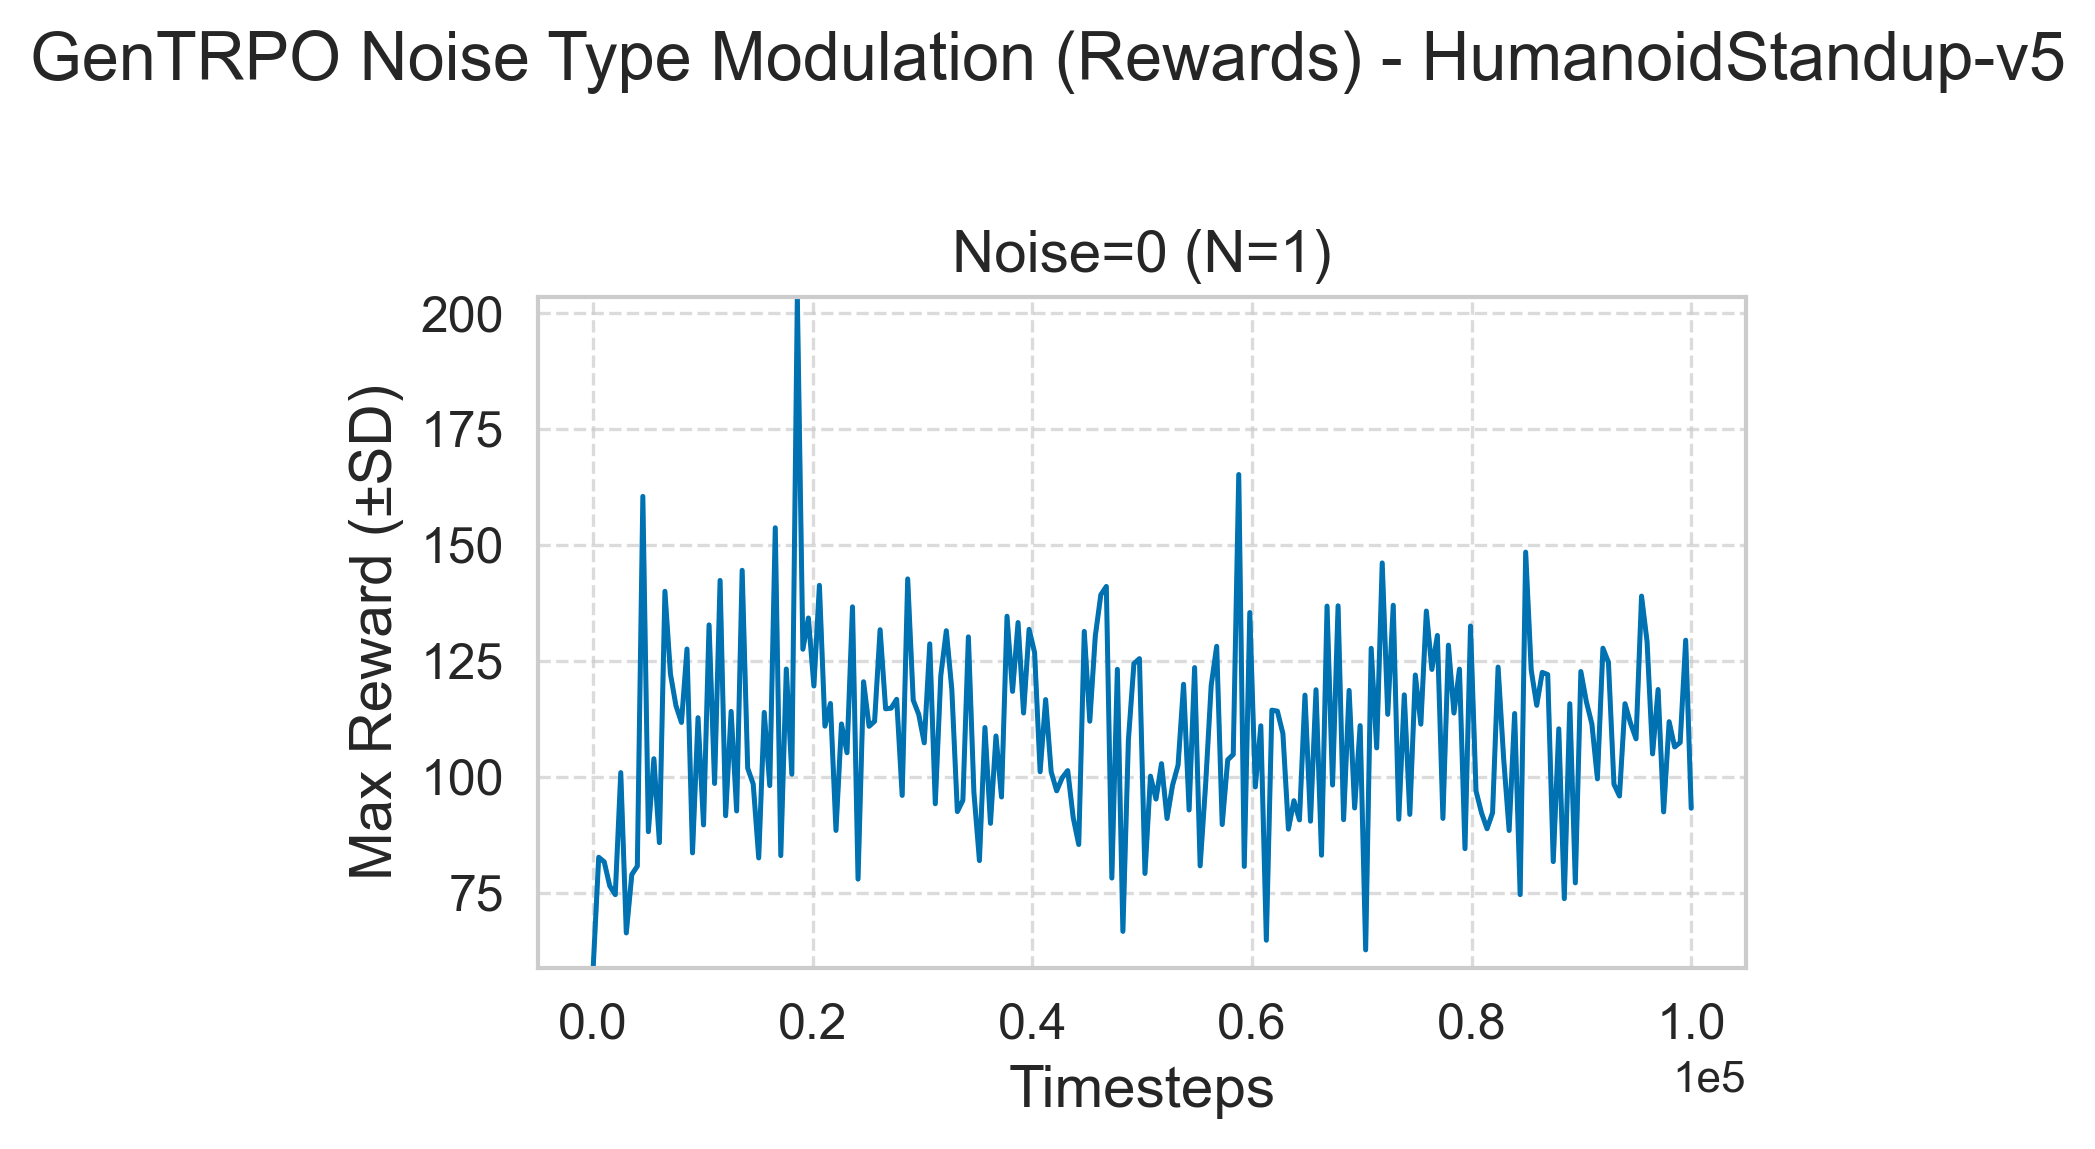
\includegraphics[width=0.8\textwidth]{graph_HumanoidStandup-v5_GenTRPO_noise_mod_rewards_grid.png}
\captionof{figure}{Noise modulation grid for rewards in GenTRPO for HumanoidStandup-v5.}
\end{center}

The grid plot for GenTRPO entropies across noise levels in HumanoidStandup-v5.

\begin{center}
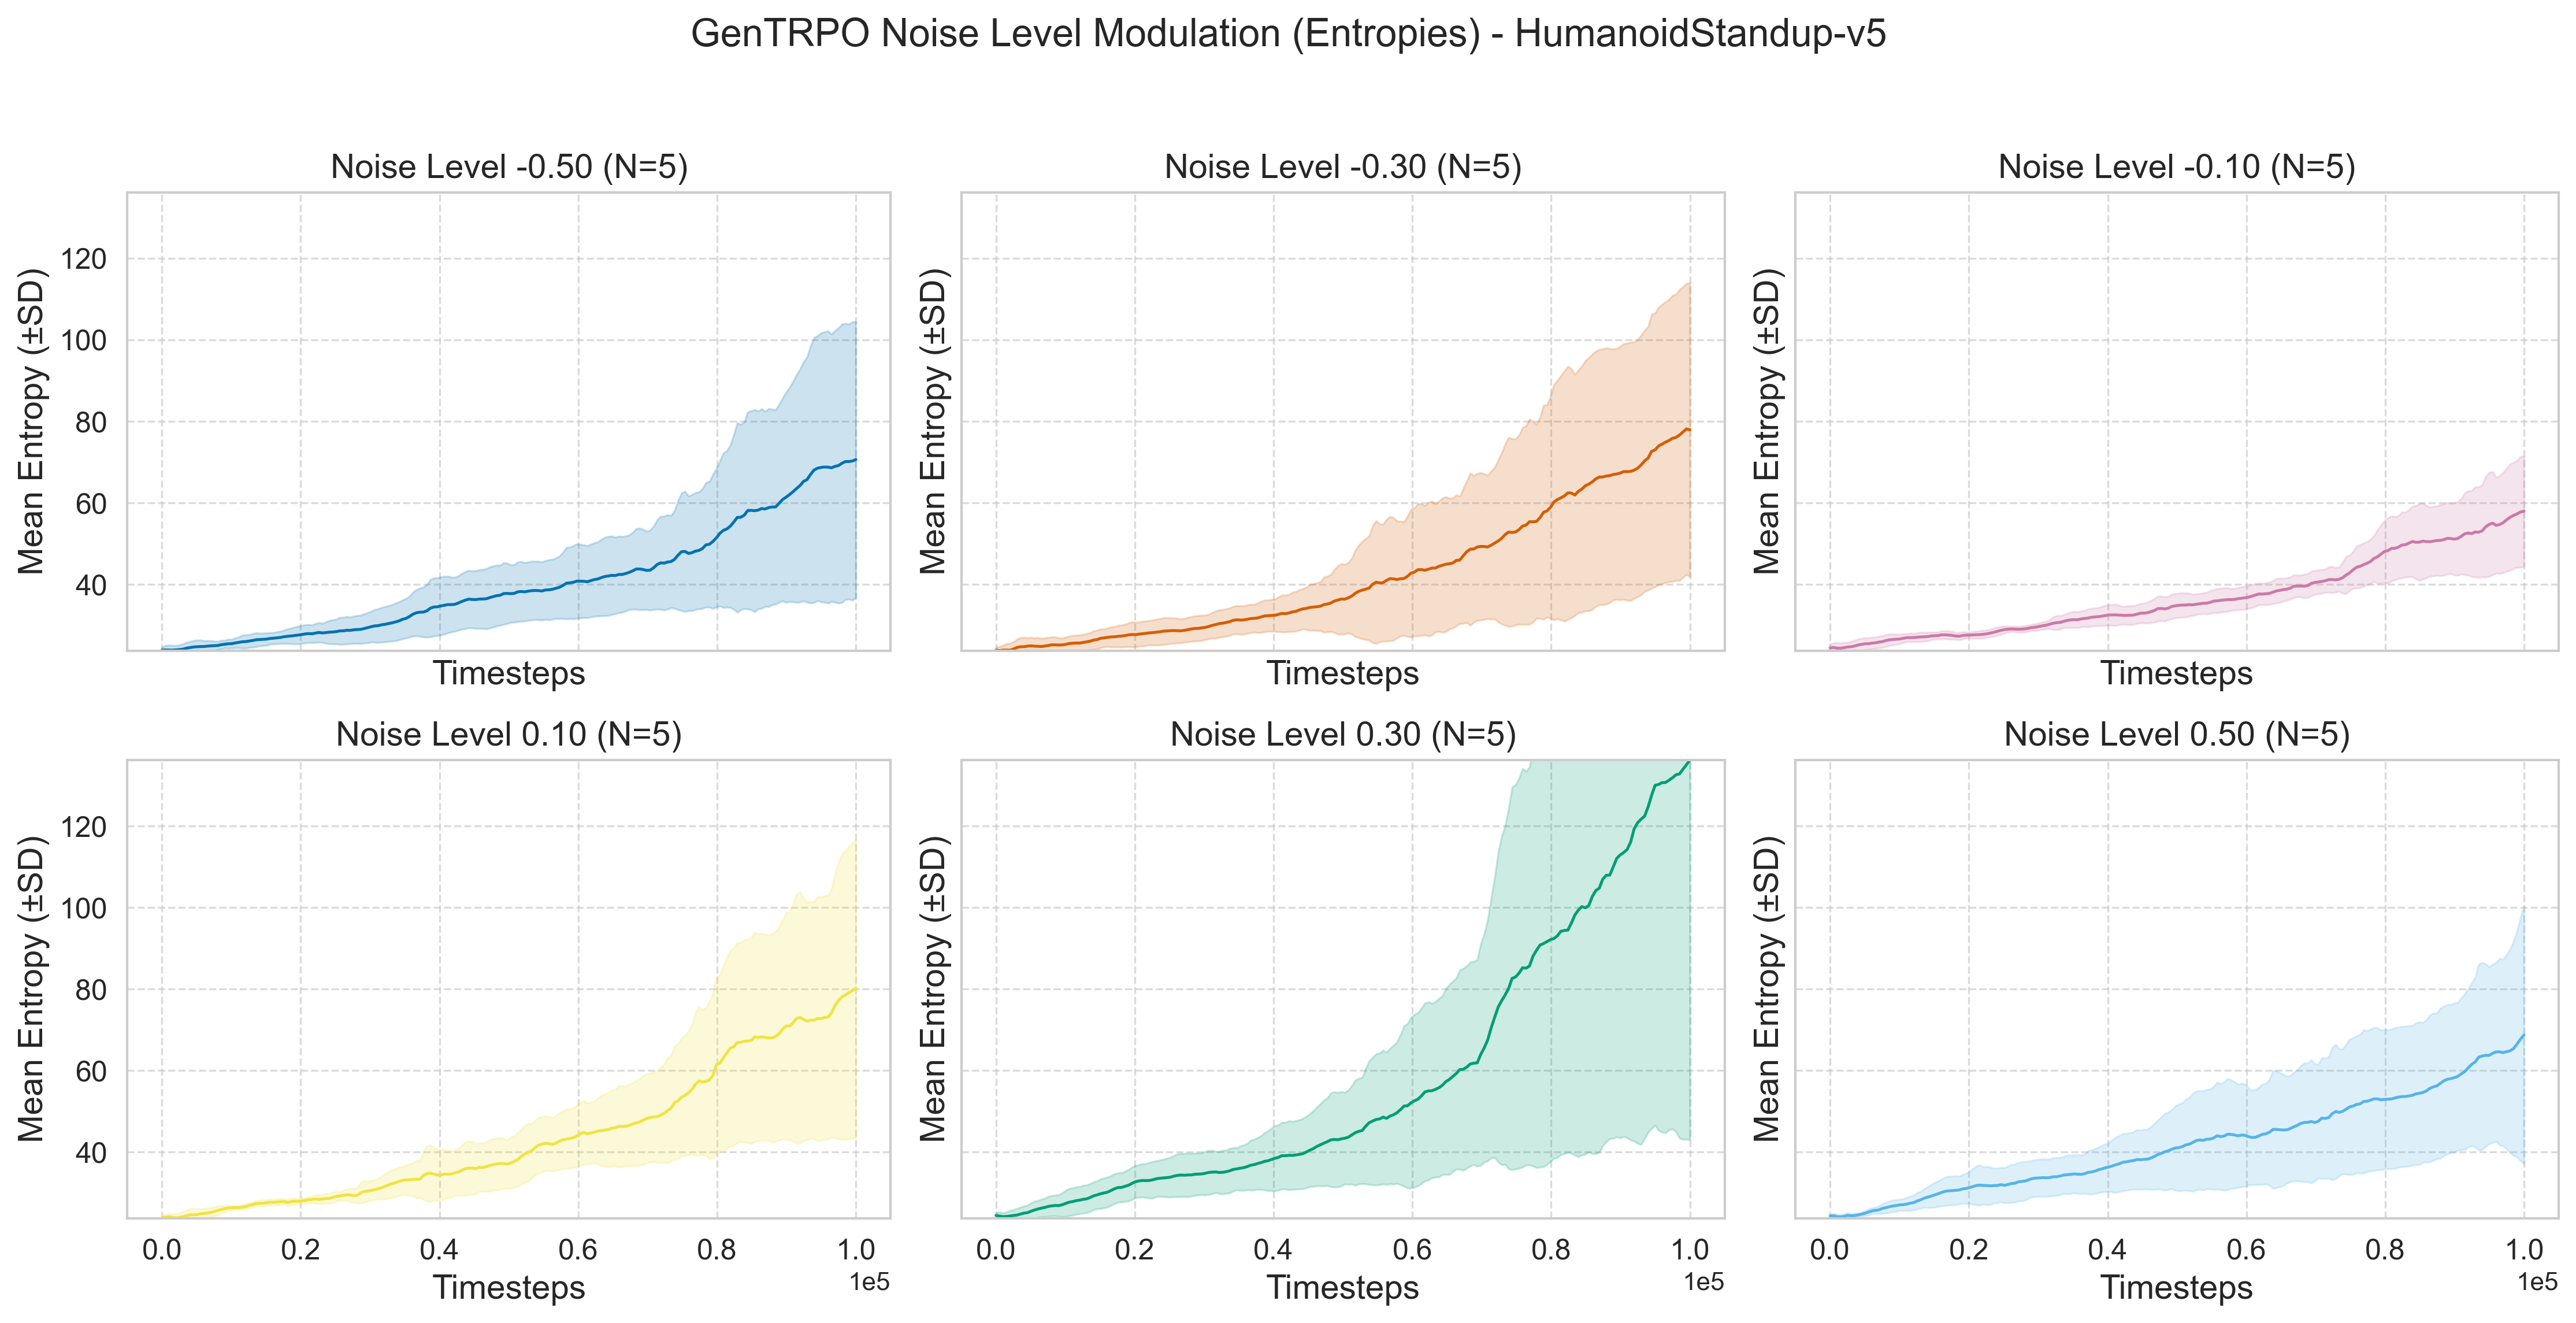
\includegraphics[width=0.8\textwidth]{graph_HumanoidStandup-v5_GenTRPO_noise_mod_entropies_grid.png}
\captionof{figure}{Noise modulation grid for entropies in GenTRPO for HumanoidStandup-v5.}
\end{center}

The grid plot for TRPO rewards across noise levels in HumanoidStandup-v5.

\begin{center}
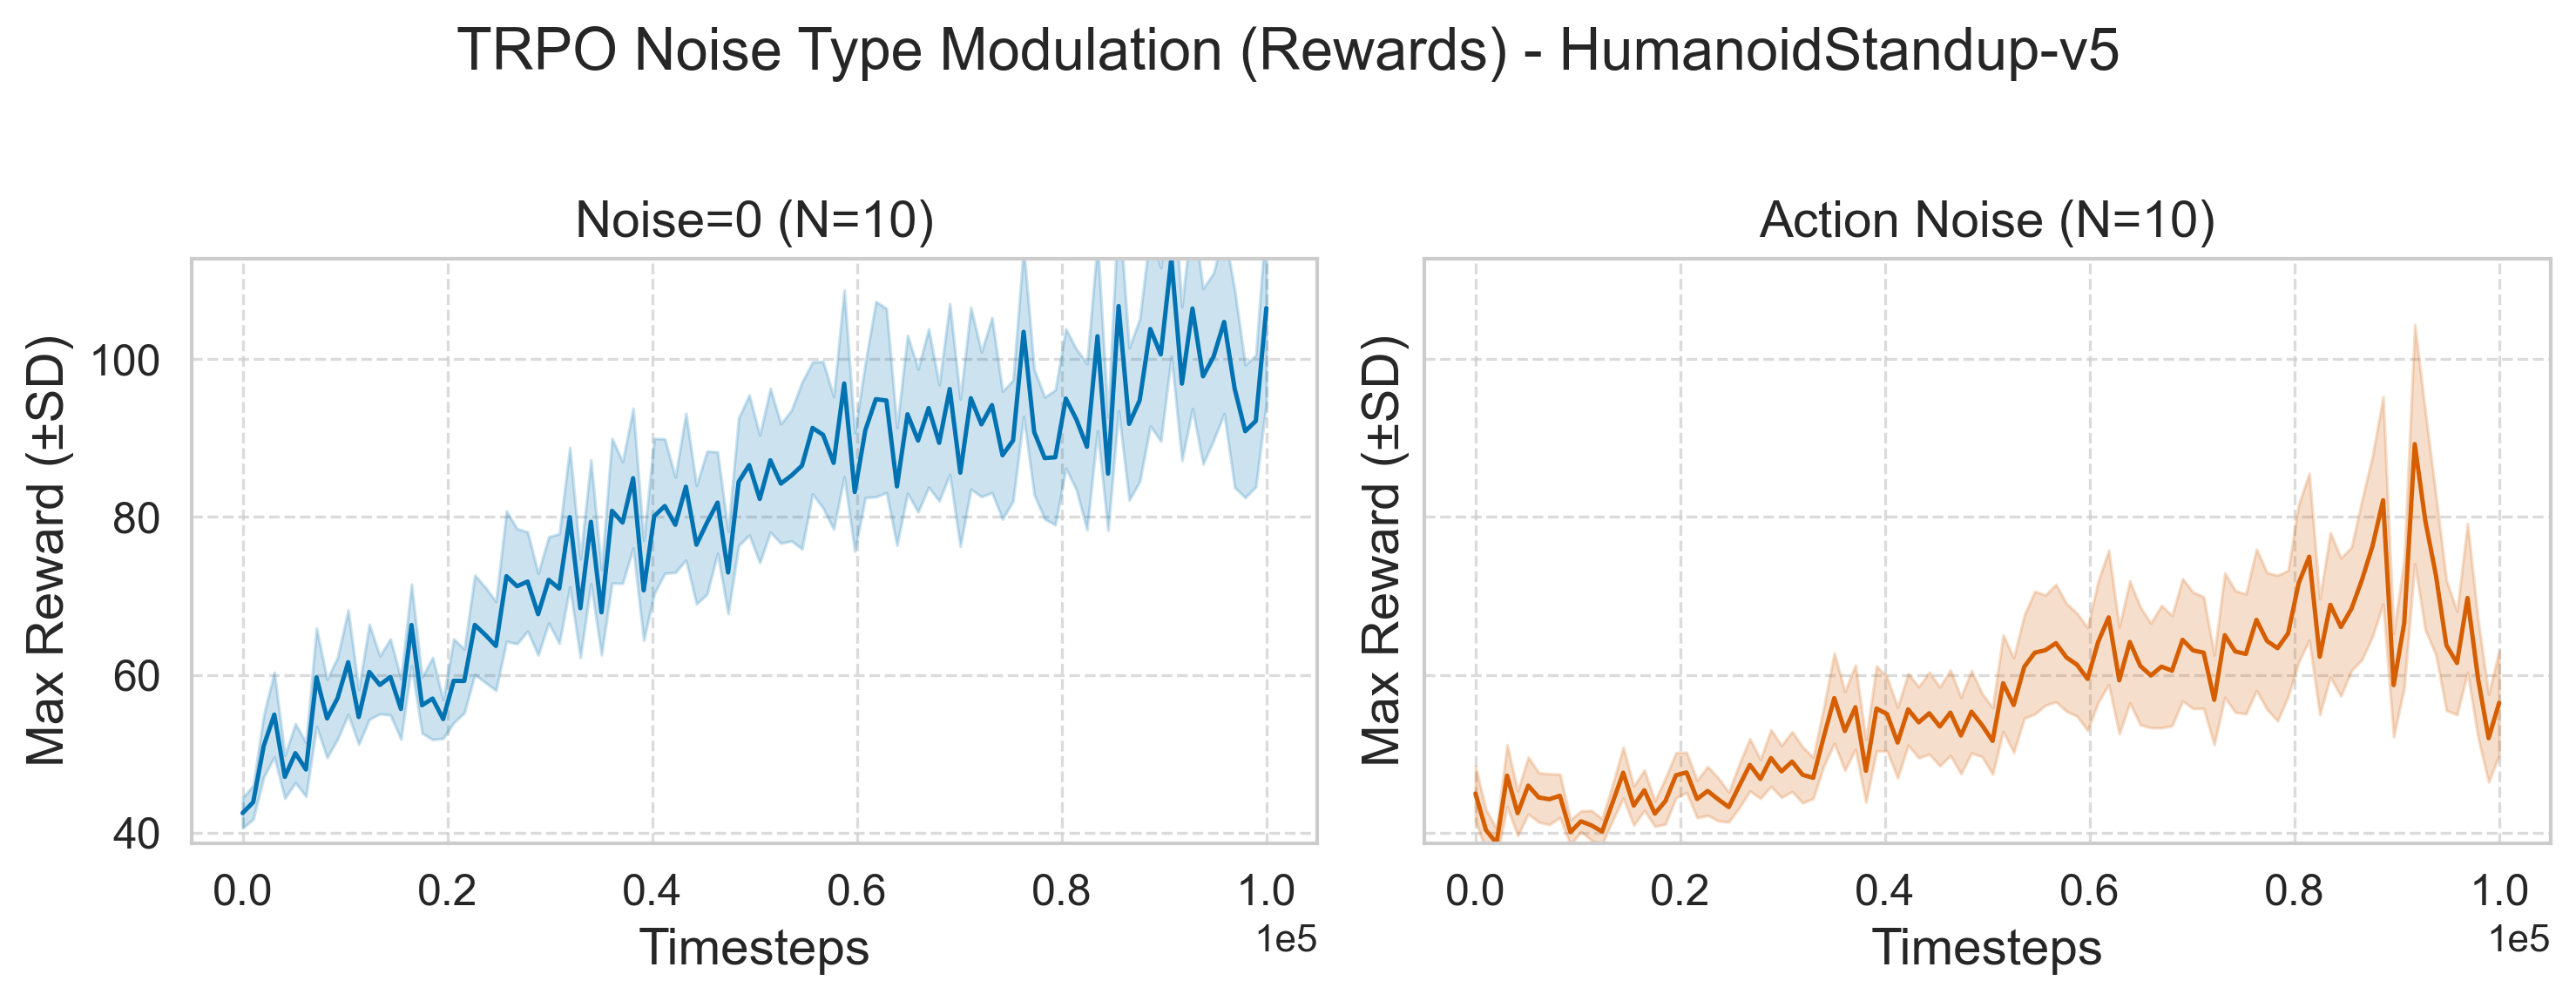
\includegraphics[width=0.8\textwidth]{graph_HumanoidStandup-v5_TRPO_noise_mod_rewards_grid.png}
\captionof{figure}{Noise modulation grid for rewards in TRPO for HumanoidStandup-v5.}
\end{center}

The grid plot for TRPO entropies across noise levels in HumanoidStandup-v5.

\begin{center}
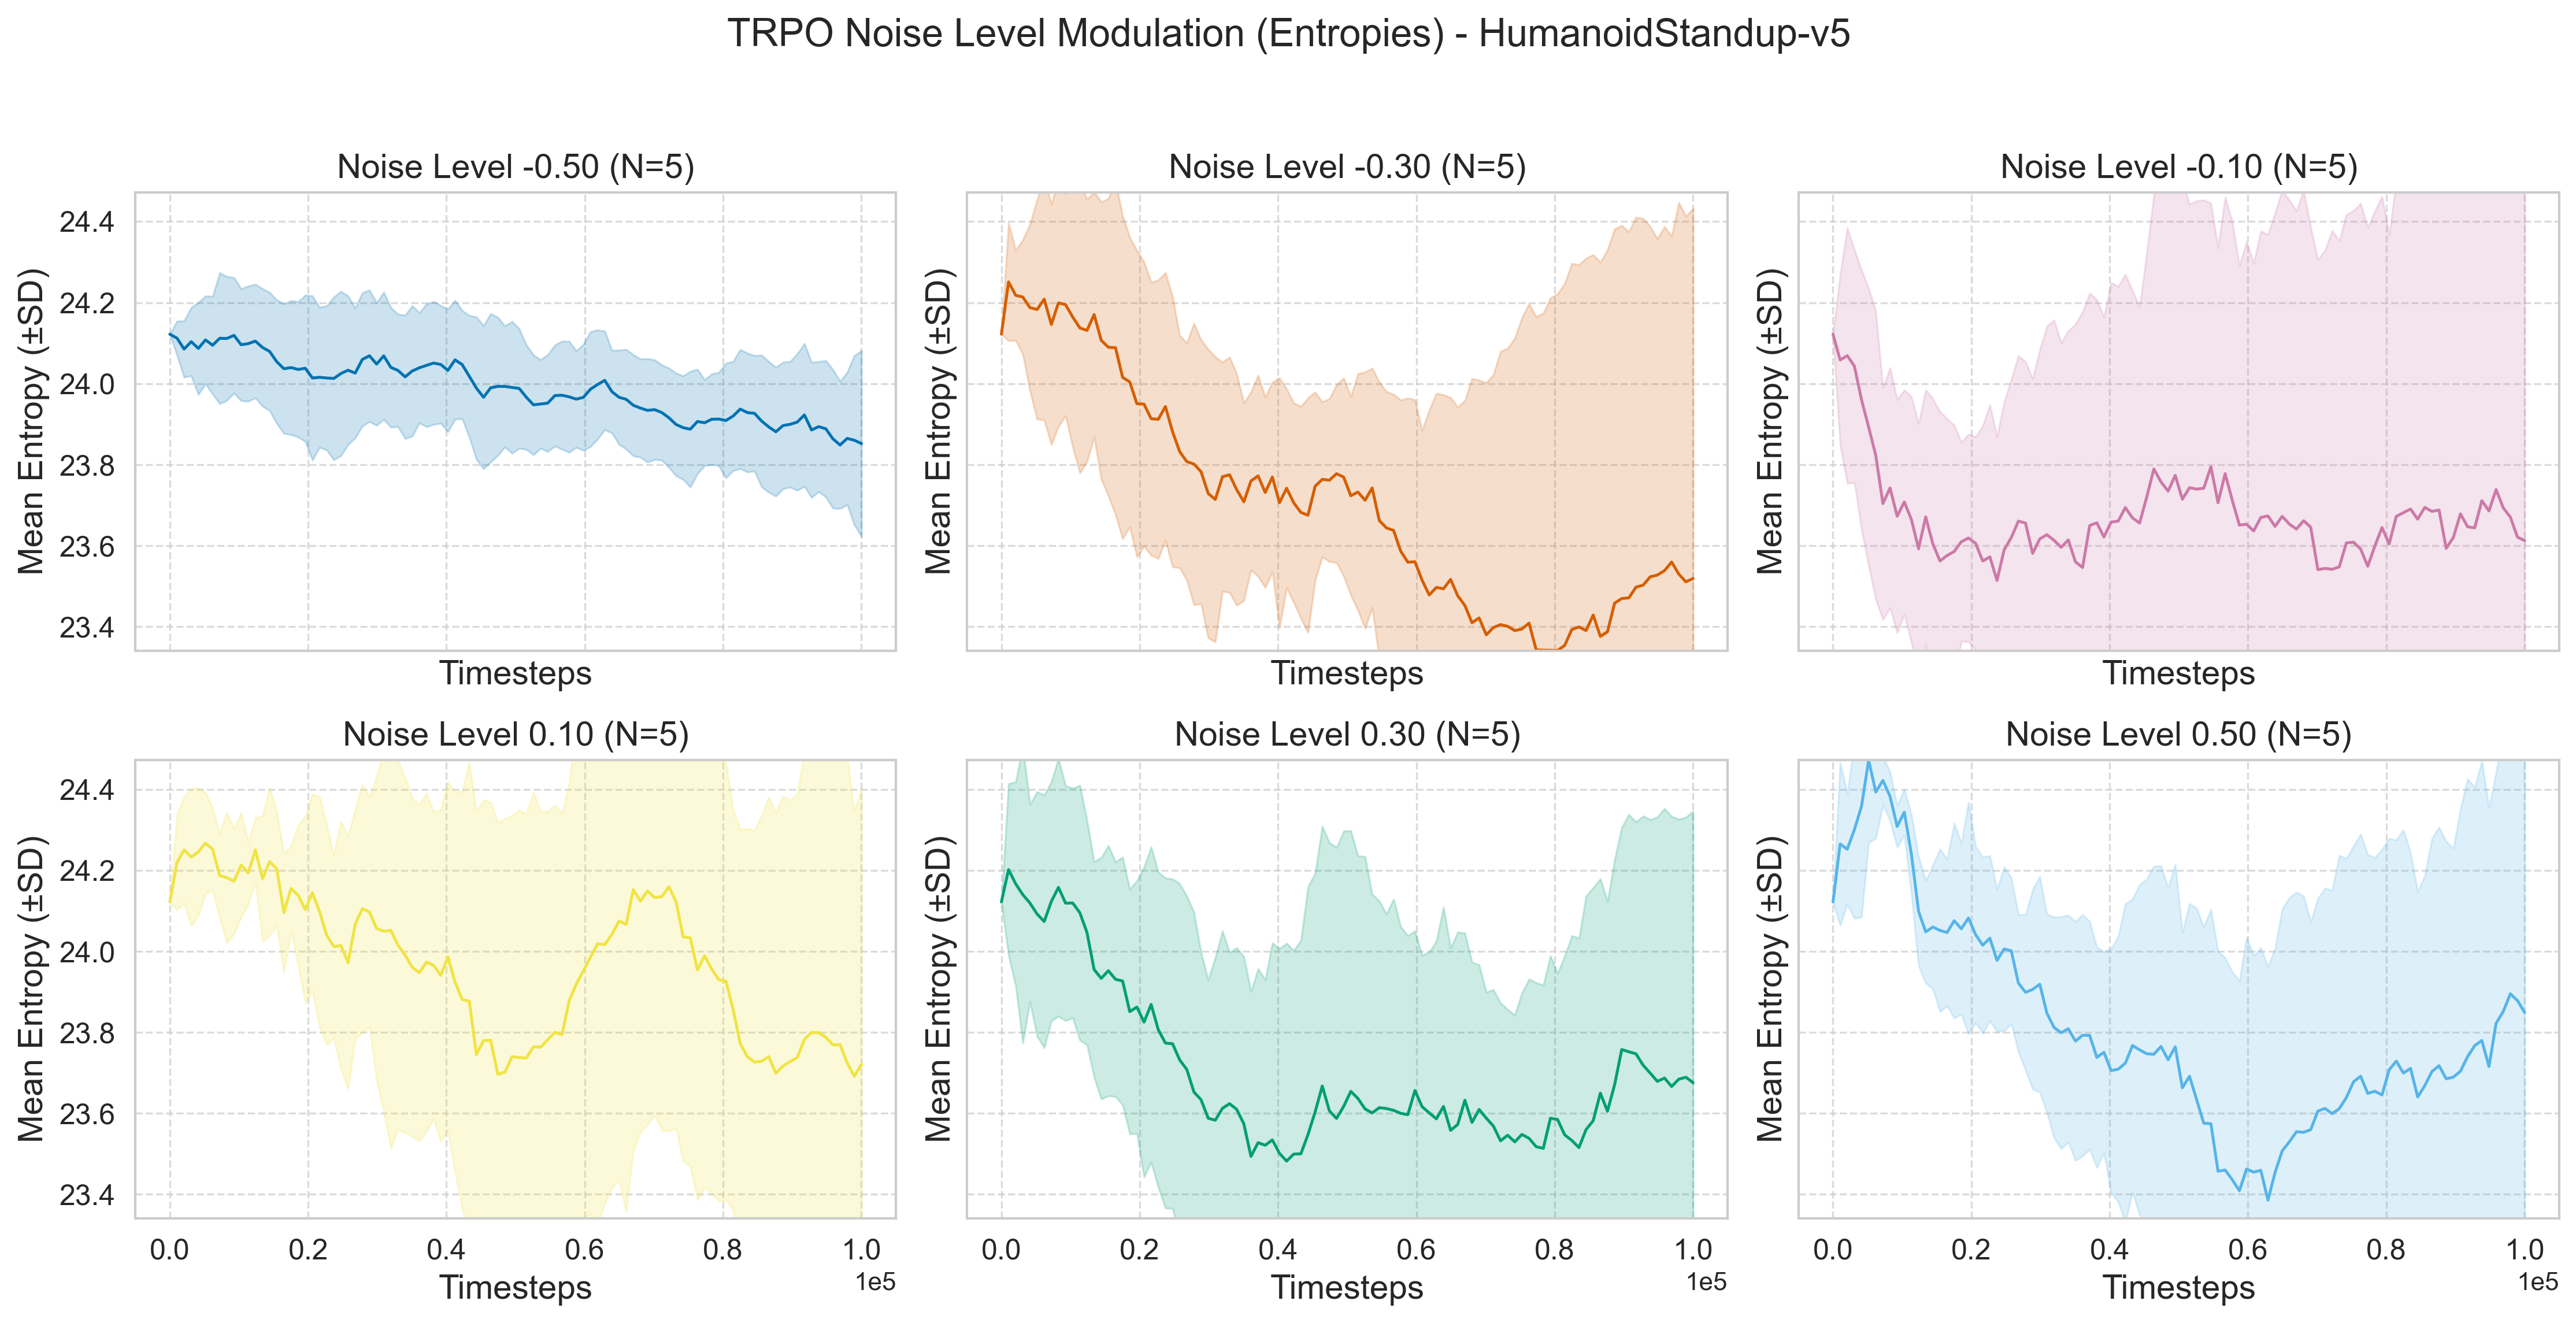
\includegraphics[width=0.8\textwidth]{graph_HumanoidStandup-v5_TRPO_noise_mod_entropies_grid.png}
\captionof{figure}{Noise modulation grid for entropies in TRPO for HumanoidStandup-v5.}
\end{center}

\subsection{Grid Plots per Environment}
These grid plots compile the rewards and entropies for a single environment across all models, offering a per-environment overview.

The grid plot for Humanoid-v5 displays rewards and entropies across different models in a grid format.

\begin{center}
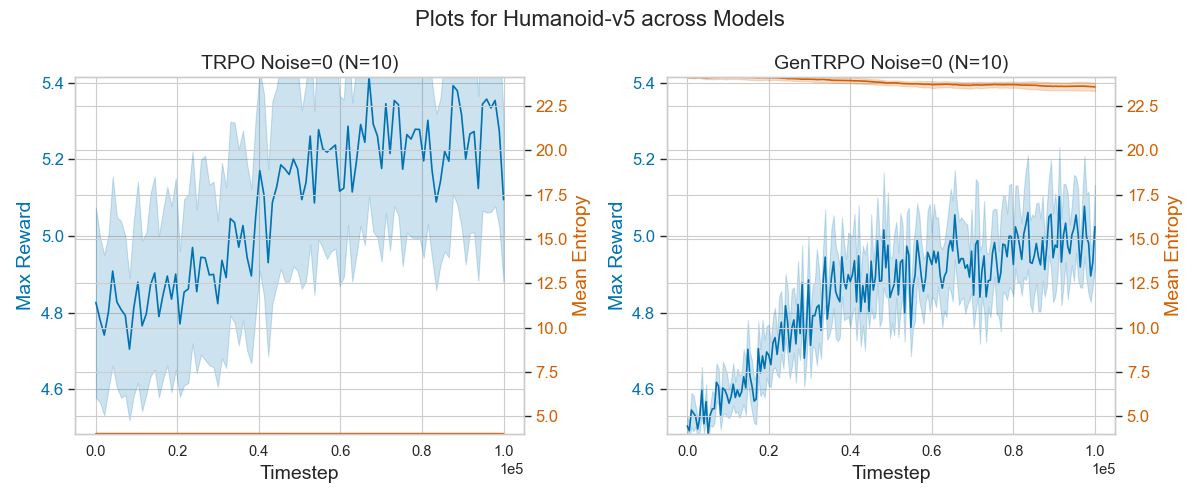
\includegraphics[width=0.8\textwidth]{grid_env_Humanoid-v5.png}
\captionof{figure}{Grid of plots for Humanoid-v5 across all models.}
\end{center}

The grid plot for HumanoidStandup-v5 displays rewards and entropies across different models in a grid format.

\begin{center}
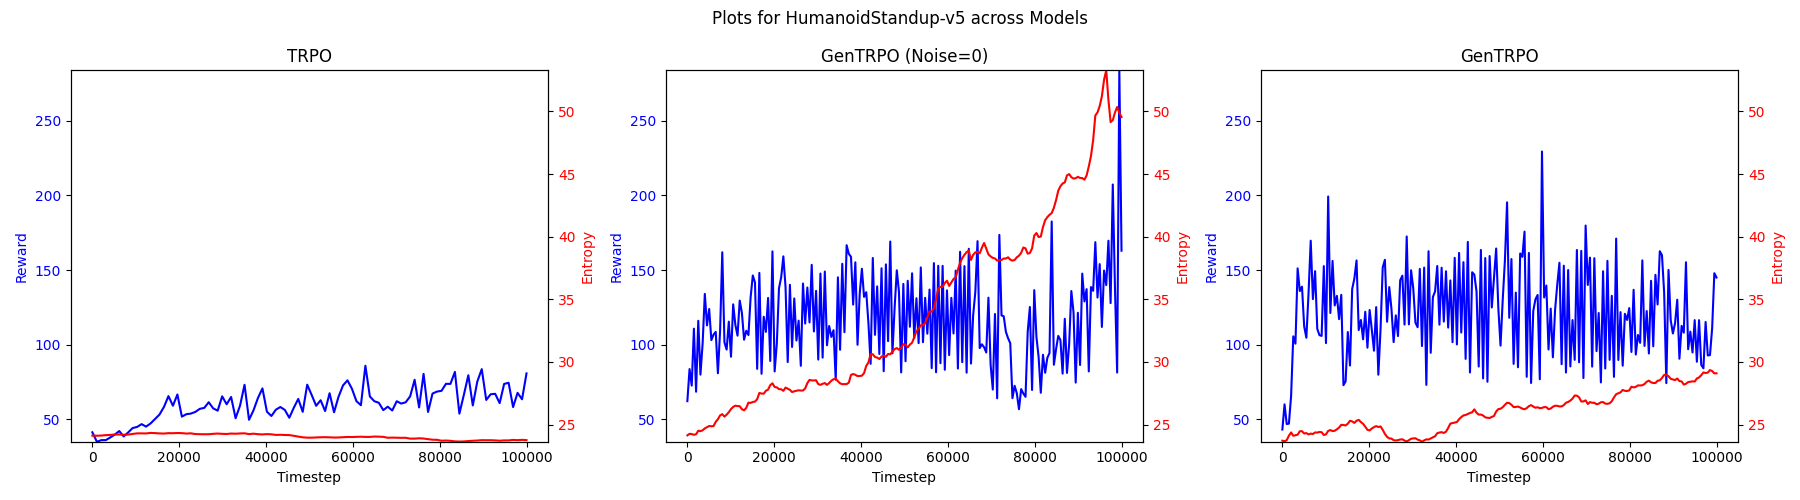
\includegraphics[width=0.8\textwidth]{grid_env_HumanoidStandup-v5.png}
\captionof{figure}{Grid of plots for HumanoidStandup-v5 across all models.}
\end{center}

\subsection{Statistics Tables}
The following tables present the detailed statistics for each model and environment combination.

\subsubsection{Statistics for TRPO in Humanoid-v5}
\begin{tabular}{lrrrrrrrrrrrrrrrrrrrrrrrrrrrr}
\toprule
Statistic & Minimum Reward & Maximum Reward & Final Reward & Timestep at Maximum & Mean Reward & Reward Standard Deviation & Median Reward & Reward Interquartile Range & Cumulative Reward & Area Under Reward Curve & Normalized Area Under Reward Curve & Coefficient of Variation Reward & Volatility & Steps to Threshold & Plateau Length & Reward Trend Slope & Reward Trend R Value & Reward Trend P Value & Reward Trend Standard Error & ROC AUC & Minimum Entropy & Maximum Entropy & Mean Entropy & Entropy Standard Deviation & Entropy Trend Slope & Entropy Trend R Value & Entropy Trend P Value & Entropy Trend Standard Error \\
Noise Type &  &  &  &  &  &  &  &  &  &  &  &  &  &  &  &  &  &  &  &  &  &  &  &  &  &  &  &  \\
\midrule
\textbf{none} & 4.38 & 4.72 & 4.70 & 96938.78 & 4.58 & 0.10 & 4.62 & 0.17 & 448.91 & 458106.50 & 0.97 & 0.02 & 0.02 & 0.00 & 2 & 0.00 & 0.96 & 0.00 & 0.00 & 1.00 & 4.01 & 4.01 & 4.01 & 0.00 & -0.00 & -0.79 & 0.00 & 0.00 \\
\textbf{action} & 4.39 & 4.68 & 4.65 & 77551.02 & 4.55 & 0.09 & 4.57 & 0.15 & 446.07 & 455190.23 & 0.97 & 0.02 & 0.02 & 0.00 & 2 & 0.00 & 0.96 & 0.00 & 0.00 & 1.00 & 4.01 & 4.01 & 4.01 & 0.00 & -0.00 & -0.78 & 0.00 & 0.00 \\
\bottomrule
\end{tabular}


\subsubsection{Statistics for GenTRPO (Noise=0) in Humanoid-v5}
\begin{tabular}{lrrrrrrrrrrrrrrrrrrrrrrrrrrrr}
\toprule
Statistic & Minimum Reward & Maximum Reward & Final Reward & Timestep at Maximum & Mean Reward & Reward Standard Deviation & Median Reward & Reward Interquartile Range & Cumulative Reward & Area Under Reward Curve & Normalized Area Under Reward Curve & Coefficient of Variation Reward & Volatility & Steps to Threshold & Plateau Length & Reward Trend Slope & Reward Trend R Value & Reward Trend P Value & Reward Trend Standard Error & ROC AUC & Minimum Entropy & Maximum Entropy & Mean Entropy & Entropy Standard Deviation & Entropy Trend Slope & Entropy Trend R Value & Entropy Trend P Value & Entropy Trend Standard Error \\
Noise Type &  &  &  &  &  &  &  &  &  &  &  &  &  &  &  &  &  &  &  &  &  &  &  &  &  &  &  &  \\
\midrule
\textbf{none} & 4.45 & 4.87 & 4.81 & 94897.96 & 4.69 & 0.12 & 4.72 & 0.17 & 919.15 & 468968.89 & 0.96 & 0.03 & 0.03 & 0.00 & 2 & 0.00 & 0.92 & 0.00 & 0.00 & 1.00 & 23.58 & 24.15 & 23.86 & 0.19 & -0.00 & -0.97 & 0.00 & 0.00 \\
\bottomrule
\end{tabular}


\subsubsection{Statistics for GenTRPO in Humanoid-v5}
\begin{tabular}{lr}
\toprule
 & Value \\
Statistic &  \\
\midrule
\textbf{max\_reward} & 5.29 \\
\textbf{timestep\_at\_max} & 90816.33 \\
\textbf{mean\_reward} & 4.92 \\
\textbf{std\_reward} & 0.20 \\
\textbf{median\_reward} & 4.97 \\
\textbf{iqr\_reward} & 0.26 \\
\textbf{cum\_reward} & 964.42 \\
\textbf{reward\_trend\_slope} & 0.00 \\
\textbf{reward\_trend\_r\_value} & 0.85 \\
\textbf{mean\_entropy} & 16.96 \\
\textbf{std\_entropy} & 2.87 \\
\textbf{min\_entropy} & 13.15 \\
\textbf{max\_entropy} & 24.12 \\
\bottomrule
\end{tabular}


\subsubsection{Statistics for TRPO in HumanoidStandup-v5}
\begin{tabular}{lrrrrrrrrrrrrrrrrrrrrrrrrrrrr}
\toprule
Statistic & Minimum Reward & Maximum Reward & Final Reward & Timestep at Maximum & Mean Reward & Reward Standard Deviation & Median Reward & Reward Interquartile Range & Cumulative Reward & Area Under Reward Curve & Normalized Area Under Reward Curve & Coefficient of Variation Reward & Volatility & Steps to Threshold & Plateau Length & Reward Trend Slope & Reward Trend R Value & Reward Trend P Value & Reward Trend Standard Error & ROC AUC & Minimum Entropy & Maximum Entropy & Mean Entropy & Entropy Standard Deviation & Entropy Trend Slope & Entropy Trend R Value & Entropy Trend P Value & Entropy Trend Standard Error \\
Noise Type &  &  &  &  &  &  &  &  &  &  &  &  &  &  &  &  &  &  &  &  &  &  &  &  &  &  &  &  \\
\midrule
\textbf{none} & 39.34 & 86.76 & 82.01 & 84693.88 & 65.91 & 12.92 & 68.62 & 21.97 & 6459.51 & 6596671.35 & 0.76 & 0.20 & 2.42 & 72448.98 & 2 & 0.00 & 0.97 & 0.00 & 0.00 & 1.00 & 38.97 & 38.99 & 38.98 & 0.01 & -0.00 & -0.83 & 0.00 & 0.00 \\
\bottomrule
\end{tabular}


\subsubsection{Statistics for GenTRPO (Noise=0) in HumanoidStandup-v5}
\begin{tabular}{lr}
\toprule
 & Value \\
Statistic &  \\
\midrule
\textbf{max\_reward} & 283.75 \\
\textbf{timestep\_at\_max} & 99400.00 \\
\textbf{mean\_reward} & 68.20 \\
\textbf{std\_reward} & 21.69 \\
\textbf{median\_reward} & 68.50 \\
\textbf{iqr\_reward} & 21.31 \\
\textbf{cum\_reward} & 852489.55 \\
\textbf{reward\_trend\_slope} & 0.00 \\
\textbf{reward\_trend\_r\_value} & 0.01 \\
\textbf{mean\_entropy} & 34.03 \\
\textbf{std\_entropy} & 7.49 \\
\textbf{min\_entropy} & 23.55 \\
\textbf{max\_entropy} & 53.96 \\
\bottomrule
\end{tabular}


\subsubsection{Statistics for GenTRPO in HumanoidStandup-v5}
\begin{tabular}{lr}
\toprule
 & Value \\
Statistic &  \\
\midrule
\textbf{max\_reward} & 229.41 \\
\textbf{timestep\_at\_max} & 59896.00 \\
\textbf{mean\_reward} & 69.26 \\
\textbf{std\_reward} & 24.21 \\
\textbf{median\_reward} & 69.69 \\
\textbf{iqr\_reward} & 23.61 \\
\textbf{cum\_reward} & 865735.37 \\
\textbf{reward\_trend\_slope} & 0.00 \\
\textbf{reward\_trend\_r\_value} & 0.10 \\
\textbf{mean\_entropy} & 26.05 \\
\textbf{std\_entropy} & 1.66 \\
\textbf{min\_entropy} & 23.35 \\
\textbf{max\_entropy} & 29.55 \\
\bottomrule
\end{tabular}


\subsection{Detailed Metrics Table}
The following table presents detailed metrics for all model-environment pairs, including maximum reward, mean reward with standard deviation, timestep at maximum reward, end slope of the reward curve, entropy trend, and entropy rate at maximum reward point.

\begin{table}[htbp]
\centering
\caption{Detailed Metrics for All Model-Environment Pairs}
\resizebox{\textwidth}{!}{
\begin{tabular}{|l|l|c|c|c|c|l|c|}
\hline
Environment & Model & Max Reward & Mean Reward ($\pm$ std) & Timestep at Max & End Slope & Entropy Trend & Entropy Rate at Max \\
\hline
Humanoid-v5 & TRPO & 4.95 & $4.76 \pm 0.14$ & 42857 & -0.0143 & decreasing & 0.0246 \\
Humanoid-v5 & GenTRPO (Noise=0) & 5.25 & $4.94 \pm 0.22$ & 95408 & -0.0038 & decreasing & -0.0147 \\
Humanoid-v5 & GenTRPO & 5.29 & $4.92 \pm 0.20$ & 90816 & 0.0099 & decreasing & -0.0250 \\
\hline
HumanoidStandup-v5 & TRPO & 85.94 & $60.15 \pm 11.13$ & 62245 & 0.8030 & decreasing & -0.0076 \\
HumanoidStandup-v5 & GenTRPO (Noise=0) & 283.75 & $68.20 \pm 21.69$ & 99400 & 5.6054 & increasing & -0.1475 \\
HumanoidStandup-v5 & GenTRPO & 229.41 & $69.26 \pm 24.21$ & 59896 & -1.9069 & increasing & -0.0008 \\
\hline
\end{tabular}
}
\end{table}
\subsection{Correlation Matrices}
The following tables show the correlation coefficients and p-values for noise level vs rewards and entropy vs rewards for each model and environment where raw data is available.

\subsubsection{Correlation Matrix for Humanoid-v5}
\begin{tabular}{lrrrr}
\toprule
Model & Noise vs Reward R & Noise vs Reward P & Entropy vs Reward R & Entropy vs Reward P \\
\midrule
TRPO & 0.06 & 0.73 & 0.24 & 0.16 \\
GenTRPO (Noise=0) & 0.16 & 0.37 & -0.26 & 0.13 \\
\bottomrule
\end{tabular}


\subsubsection{Correlation Matrix for HumanoidStandup-v5}
\begin{tabular}{lrrrr}
\toprule
Model & Noise vs Reward R & Noise vs Reward P & Entropy vs Reward R & Entropy vs Reward P \\
\midrule
TRPO & 0.35 & 0.04 & -0.29 & 0.09 \\
GenTRPO (Noise=0) & -0.22 & 0.21 & -0.68 & 0.00 \\
\bottomrule
\end{tabular}


\end{document}